\documentclass[12pt,a4paper,oneside]{report}
% =========================================================
% Language
% =========================================================
\usepackage[T1]{fontenc}
\usepackage[ngerman]{babel}
% =========================================================
% Stildefinitionen für Blockschaltbilder
% =========================================================
\usepackage{newtxtext,newtxmath}
\usepackage{tikz}
\usetikzlibrary{arrows.meta, positioning, calc, fit, backgrounds}
\tikzset{
  blk/.style={
    draw, rounded corners=1.5pt, thick,
    minimum height=10mm, text width=16mm,
    align=center, font=\scriptsize,
    fill=black!3
  },
  blkw/.style={blk, text width=28mm},
  msg/.style={blk, text width=40mm, fill=black!8},
  sum/.style={
    draw, circle, thick, minimum size=6mm,
    inner sep=0pt, font=\small
  },
  ghost/.style={
    draw, circle, thick, dashed, minimum size=6mm,
    inner sep=0pt, font=\small, text=black!55
  },
  sig/.style={-{Latex[length=2mm,width=1.6mm]}, thick},
  line/.style={thick},
  miss/.style={-{Latex[length=2mm,width=1.6mm]}, thick, dashed, black!55},
  lbl/.style={font=\scriptsize},
  grp/.style={font=\scriptsize, text=black!55}
}
 
% =========================================================
% Page Layout
% =========================================================
\usepackage[a4paper,
left=3.5cm,
right=2.5cm,
top=3cm,
bottom=2.5cm]{geometry}
\usepackage{setspace}
\onehalfspacing
\setlength{\parindent}{1.2em}
\setlength{\parskip}{0pt}
\setlength{\parindent}{0pt}
\usepackage{tcolorbox}
\tcbset{
  colback=gray!10,
  colframe=black,
  boxrule=0.5pt,
  arc=3pt
}
% =========================================================
% Header and Footer 
% =========================================================
\usepackage{fancyhdr}
\pagestyle{fancy}
\fancyhf{}
\renewcommand{\chaptermark}[1]{\markboth{\thechapter\ #1}{}}
% Kapitelname + Nummer im Header links
\fancyhead[L]{\nouppercase{\leftmark}}
% Seitenzahl im Footer (zentriert)
\fancyfoot[C]{\thepage}
% Linien
\renewcommand{\headrulewidth}{0.4pt}
\renewcommand{\footrulewidth}{0.4pt}
% Kapitelanfangsseiten auch mit Header!
\usepackage{etoolbox}
\patchcmd{\chapter}{\thispagestyle{plain}}{\thispagestyle{fancy}}{}{}
% =========================================================
% Math, Tables, Code
% =========================================================
\usepackage{amsmath}
\usepackage{booktabs}
\usepackage{listings}
\usepackage{xcolor}
\usepackage{siunitx}
\sisetup{locale=DE}
% =========================================================
% Figures
% =========================================================
\usepackage{graphicx}
\usepackage{caption}
\usepackage{subcaption}
\captionsetup{
font=small,
labelfont=bf
}
% =========================================================
% Hyperlinks
% =========================================================
\PassOptionsToPackage{hyphens}{url} % Erzwingt Umbrüche bei Bindestrichen
\usepackage{hyperref}
\hypersetup{
colorlinks=true,
linkcolor=black,
urlcolor=blue,
citecolor=black
}
\usepackage{cleveref}
\usepackage{hyperref}
\usepackage{url}
% =========================================================
% Code Style (angepasst auf C / Embedded)
% =========================================================
\definecolor{codeblue}{rgb}{0.1,0.1,0.7}
\definecolor{codegreen}{rgb}{0,0.5,0}
\definecolor{codegray}{rgb}{0.4,0.4,0.4}
\lstset{
language=C,
basicstyle=\ttfamily\footnotesize,
keywordstyle=\color{codeblue}\bfseries,
commentstyle=\color{codegray}\itshape,
stringstyle=\color{codegreen},
numbers=left,
numberstyle=\tiny,
frame=single,
breaklines=true,
breakatwhitespace=true,
tabsize=2,
showstringspaces=false
}
% =========================================================
% Chapter Style
% =========================================================
\usepackage{titlesec}
\titleformat{\chapter}
{\normalfont\huge\bfseries}
{\thechapter.}{1em}{}
% =========================================================
% Other Packages
% =========================================================
\usepackage{ragged2e}
\usepackage{microtype}
\usepackage{tikz}
\usetikzlibrary{arrows.meta, positioning}
\usepackage{svg}
\usepackage{csquotes}
\usepackage[printonlyused]{acronym}
% =========================================================
\begin{document}
\justifying
\titlespacing*{\chapter}{0pt}{0pt}{20pt}
% =========================================================
% Title Page
% =========================================================
\begin{titlepage}
\centering
\vspace*{1cm}

\includegraphics[width=0.5\textwidth]{Abbildung/Frankfurt_University_of_Applied_Sciences_logo.png}\\[1.5cm]
{\Large \textbf{Projektarbeit}}\\[1cm]
{\huge \textbf{Entwicklung einer Positions- und}}\\[0.5cm]
{\huge \textbf{Drehmomentregelung für einen Greifer}}\\[0.5cm]
{\Large \textbf{(FRoST-Endeffektor)}}\\[2cm]
\textbf{Studiengang:} Mechatronik und Robotik M.Sc.\\
\textbf{Modul:} Simulation und Regelung\\[0.5cm]
\textbf{Dozent:} Prof.~Dr.~K.~Schmidt\\[1.5cm]
\textbf{Vorgelegt am:} \textit{14.09.2026}\\
im Sommersemester 2026\\[1cm]
\textbf{Bearbeitet von:}\\[1cm]
\begin{tabular}{c c}
\bottomrule \textbf{Name} & \textbf{Matrikelnummer} \\
\midrule
\textit{Masoud Fahim}           &   \textit{1208212} \\
\textit{Mohammad Badr Eddin}    &   \textit{1310838} \\
\textit{Lars Hellriegel}        &   \textit{1359307} \\
\textit{Mohamad Shaikh Khalil}  &   \textit{1654017} \\
\bottomrule
\end{tabular}
\vfill
\end{titlepage}

% =========================================================
% Eidesstattliche Erklärung
% =========================================================
\chapter*{Eidesstattliche Erklärung}
\thispagestyle{empty}
Ich versichere hiermit, dass ich die vorliegende Arbeit selbständig verfasst und keine anderen als die im Literaturverzeichnis angegebenen Quellen benutzt habe.
\medskip

\noindent
Alle Stellen, die wörtlich oder sinngemäß aus veröffentlichten oder noch nicht veröffentlichten Quellen entnommen sind, sind als solche kenntlich gemacht.
\medskip

\noindent
Die Zeichnungen oder Abbildungen in dieser Arbeit sind von mir selbst erstellt worden oder mit einem entsprechenden Quellennachweis versehen.
\medskip

\vspace{2cm}

\noindent
Frankfurt, den 14.09.2026

\vspace{2cm}

\noindent

\begin{minipage}{0.45\textwidth}
    \centering
    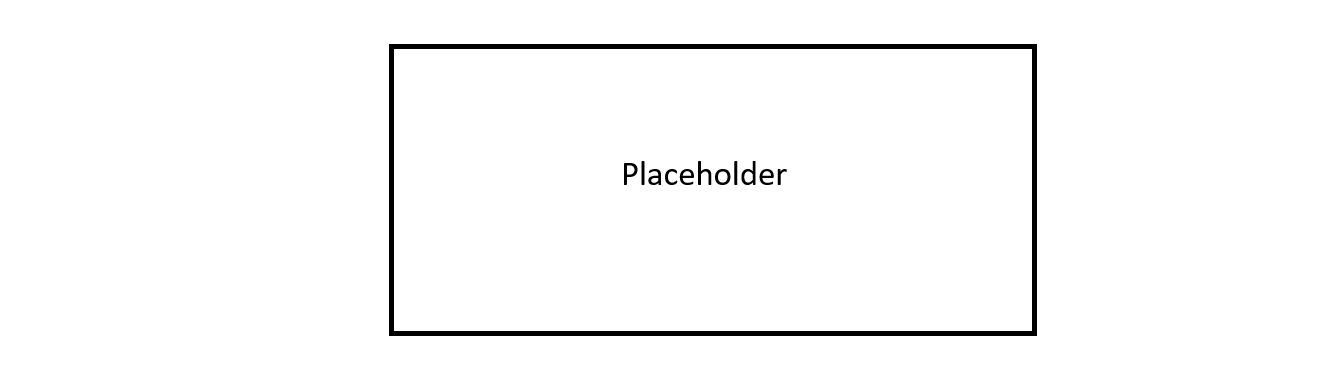
\includegraphics[width=5cm]{Abbildung/placeholder.png}\\
    \vspace{0.5cm}
    \rule{5cm}{0.4pt}\\
    Masoud Fahim
\end{minipage}
\begin{minipage}{0.45\textwidth}
    \centering
    
\includegraphics[width=5cm]{Abbildung/Signatures/Mo_signature.png}\\
    \vspace{0.5cm}
    \rule{5cm}{0.4pt}\\
    Mohammad Badr Eddin
\end{minipage}

\hfill

\begin{minipage}{0.45\textwidth}
    \centering
    \vspace{2cm}
    
\includegraphics[width=5cm]{Abbildung/Signatures/Lars_Unterschrift.png}\\
    \vspace{0.5cm}
    \rule{5cm}{0.4pt}\\
    Lars Hellriegel
\end{minipage}
\begin{minipage}{0.45\textwidth}
    \centering
    \vspace{2cm}
    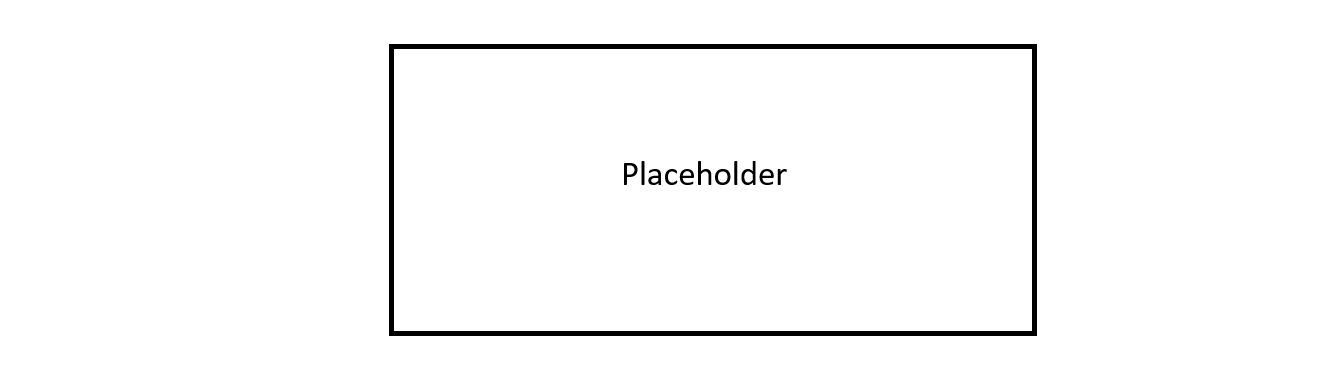
\includegraphics[width=5cm]{Abbildung/placeholder.png}\\
    \vspace{0.5cm}
    \rule{5cm}{0.4pt}\\
    Mohamad Shaikh Khalil
\end{minipage}

% =========================================================
% Verzeichnisse
% =========================================================
\pagenumbering{Roman}
\tableofcontents
\newpage
% =========================================================
%\chapter*{Abkürzungsverzeichnis}

\listoffigures
\addcontentsline{toc}{chapter}{Abbildungsverzeichnis}
\newpage
%\listoftables
%\addcontentsline{toc}{chapter}{Tabellenverzeichnis}
%\newpage


% =========================================================
% Main Part
% =========================================================
\cleardoublepage
\pagenumbering{arabic}

% ---------------------------------------------------------
% Einleitung
% ---------------------------------------------------------
\chapter{Einleitung}
% Kurzer Überblick: Kontext des Projekts (FRoST-Endeffektor), Motivation, Ziel
% (Positions- und Drehmomentregelung), und Aufbau des Berichts (Kapitelübersicht).

Die vorliegende Projektarbeit, die als Prüfungsleistung des Moduls ``Simulation und Regelung'' durchzuführen ist, lag eingangs der Thematik der Entwicklung eines Positions- und Drehmomentreglers für einen neu entwickelten FRoST-Endeffektor zugrunde. Aufgrund des Verwerfens des neuen Greifer-Konzeptes, wurde die Aufgabenstellung im Laufe der Bearbeitungszeit angepasst bzw. erweitert. Aufgrund der Absenz eines physischen Greifers, konnten Teilaspekte der Aufgabenstellung, die eine Vermessung der Mechanik voraussetzen, nicht bearbeitet werden. Zudem wurde die Entwicklung eines Prüfstandes, der die Funktionalität eines Greifers simuliert, als weiterer Bestandteil der Projektarbeit aufgenommen.\\

Das grundsätzlich (unveränderte) Ziel der Projektarbeit liegt darin, zwei Reglerkonzepte für einen Schrittmotor - dieser treibt die Finger an - zu entwickeln und praktisch umzusetzen. Es liegen lediglich vereinzelte Vorgaben hinsichtlich der verwendeten Hard- und Software vor. Durch den Positionsregler soll die Greifposition und durch den Drehmomentregler soll die Greifkraft sicher und präzise gesteuert werden können.\\

In den folgenden Kapiteln werden zuerst die Aufgabenstellung und die Anforderungen an das zu realisierende Regelsystem zusammengefasst (Kapitel \ref{Kap:Aufgabe}). Anschließend wird in Kapitel \ref{Kap:Material} die ausgewählte Hard- und Software vorgestellt. In Kapitel \ref{Kap:System} wird nachfolgend die Erarbeitung eines Entwurfs eines Prüfstandes als zu regelndes System und die daraus abgeleiteten Systemgrenzen und das daraus resultierende mathematische Modell beschrieben. In Kapitel \ref{Kap:Feedback} wird daraufhin das Auslesen des Motorfeedbacks mittels geeigneter Sensorik thematisiert. Infolgedessen werden die Entwürfe der beiden Regler in Kapitel \ref{Kap:Regler} erläutert. Die Implementierung der Firmware für das zentrale Steuergerät des Systems wird in Kapitel \ref{Kap:Firmware} beleuchtet. Um die entwickelten Regler auf ihre Funktionalität zu überprüfen, wird in Kapitel \ref{Kap:Testlauf} eingangs die Realisierung des Prüfstandes behandelt und anschließend die Einhaltung der vorgegebenen Anforderungen erörtert. Abschließend beinhaltet das Kapitel \ref{Kap:Fazit} ein Fazit und einen Ausblick.


\bigskip

% ---------------------------------------------------------
% Aufgabenstellung & Anforderungen
% ---------------------------------------------------------
\chapter{Aufgabenstellung und Anforderungen}\label{Kap:Aufgabe}
% Präzise Wiedergabe der Aufgabenstellung (Thema 6) und der geforderten
% Systemanforderungen (Echtzeitfähigkeit, Positioniergenauigkeit,
% Regelbarkeit von Greifkraft/Drehmoment, Überlast-/Kollisionsschutz,
% nahtlose Umschaltung, Wiederholgenauigkeit).
Die Bearbeitung der Projektarbeit lässt sich in die vier folgenden Teilaufgaben aufgliedern:\\
Die \textit{Charakterisierung des Systems} \textbf{(1)} sollte ursprünglich die Analyse der vorliegenden Mechanik (Übersetzung, Reibung, Spiel) sowie der Motor- und Treiberkennlinien beinhalten. Da kein physischer Greifer vorhanden ist, an dem die Analyse durchgeführt werden kann, ist eine solche Analyse nicht durchführbar. Stattdessen soll im Rahmen dieser Teilaufgabe ein Prüfstand entwickelt werden, der die für die Systemcharakterisierung notwendigen Messungen am Motor-/Treibersystem ermöglicht. Der Prüfstand bildet demnach die messtechnische Grundlage für die Ermittlung der Systemgrenzen (max. Strom, Drehmoment, Geschwindigkeit) auf Basis der am Prüfstand erfassten Motor- und Treiberkennlinien und die Erstellung eines vereinfachten mathematischen Modells als Grundlage für den nachfolgenden Reglerentwurf. \\ %\textcolor{red}{Korrekt????}
Das \textit{Auslesen des Motorfeedbacks} \textbf{(2)} umfasst die Rückführung der Regelgrößen mittels geeigneter Sensorik - anstelle der eingangs vorgeschlagenen Strommessung ist ein Encoder zu nutzen - deren aufgenommene Rohdaten aufzubereiten (Filterung, Skalierung) sind.\\
Die \textit{Entwicklung von zwei Reglern} \textbf{(3)} gibt vor, dass einerseits ein Positionsregler zur exakten Ansteuerung von Fingerstellung bzw. Öffnungsweite und andererseits ein Drehmomentregler zur indirekten oder direkten Regelung der Greifkraft über Motorstrom bzw. -drehmoment zu entwerfen ist. Die Reglerauslegung ist als PI-, PID-, oder Zustandsregelung vor der praktischen Umsetzung zu simulieren und zu parametrieren.\\
Die \textit{Umsetzung der Regler in FreeRTOS auf einem STM32H7} \textbf{(4)} konnte aufgrund eines Hardwarefehlers des H7 Boards nicht erfolgen, weshalb die Implementierung der Regler als Echtzeitanwendung auf einem STM32F7 vorzunehmen ist.\\

Des Weiteren wurden für das zu entwickelnde Regelungssystem folgende Anforderungen formuliert:

\begin{itemize}
    \item \textbf{Echtzeitfähigkeit:} Die Regelung muss mit einer definierten, deterministischen Zykluszeit (z.B. \ensuremath{\le} 1 ms) auf der Zielhardware lauffähig sein.
    \item \textbf{Positioniergenauigkeit:} Die Fingerposition muss mit einer Genauigkeit von \ensuremath{\le} ±0,5 mm (bzw. entsprechender Winkelauflösung) angefahren werden können.
    \item \textbf{Regelbare Greifkraft/Drehmoment:} Das aufgebrachte Drehmoment bzw. die Greifkraft muss in einem definierten Bereich stufenlos vorgebbar und eingeregelt werden können, um unterschiedlich empfindliche Objekte sicher greifen zu können.
    \item \textbf{Überlast- und Kollisionsschutz:} Es ist eine Strom-/Drehmomentbegrenzung sowie eine Fehlererkennung (z.B. Blockade, Übertemperatur, Schrittverlust) mit definierter Sicherheitsreaktion vorzusehen.
    \item \textbf{Nahtlose Umschaltung:} Während des Betriebs muss zwischen Positions- und Drehmomentregelung umgeschaltet werden können (z.B. positionsgeregelte Annäherung, drehmomentgeregelter Greifvorgang).
    \item \textbf{Wiederholgenauigkeit:} Das Systemverhalten muss über mehrere Greifzyklen hinweg reproduzierbar sein. Hierfür wird ein Langzeittest empfohlen.
    \item \textbf{Dokumentation:} Systemcharakterisierung, Reglerentwurf, Parametrierung und Testergebnisse sind vollständig zu dokumentieren. Ein experimenteller Vergleich beider Reglerkonzepte am realen System war aufgrund des fehlenden Greifers nicht möglich und ist entsprechend nicht Bestandteil dieser Dokumentation.
\end{itemize}

\bigskip

% ---------------------------------------------------------
% Verwendete Hard- & Software
% ---------------------------------------------------------
\chapter{Verwendete Hard- und Software}\label{Kap:Material}
% Vorstellung der verwendeten Komponenten: FRoST-Endeffektor/Greifer,
% Schrittmotor (Stepper) und Treiber, STM32H7-Microcontroller, Sensorik
% zur Strommessung, Entwicklungsumgebung (z.B. STM32CubeIDE, FreeRTOS),
% Simulationssoftware 
Die geeigneten Hardware- und Softwarekomponenten zur Durchführung der erläuterten Aufgaben unter Einhaltung der formulierten Anforderungen wurden vereinzelt bereits in der Aufgabenstellung vorgegeben. Die restlichen Komponenten wurden durch eine eingehende Recherche ausgewählt. Folgend sind die verschiedenen ausgewählten Komponenten kurz beschrieben.\\

Durch die Aufgabenstellung vorgegeben war einerseits ein Microcontroller des Typs STM32H7, der aufgrund eines Hardwarefehlers durch das verfügbare Board NUCLEO-F767ZI ersetzt wurde. Andererseits galt die Vorgabe FreeRTOS zur Implementierung des Regelungssystems zu verwenden.\\

Aufgrund des fehlenden Greifers wurde der NEMA17 17HE12-1204S Schrittmotor (1,2 A pro Phase) ausgewählt – dieser war verfügbar und für die Zwecke am Prüfstand ausreichend.\\

Für die Ansteuerung des Schrittmotors wurde der Motortreiber TMC2209 V2.0 ausgewählt, da dieser die Spezifikationen des Schrittmotors (typischerweise 2 A) komfortabel erfüllt, eine UART-Schnittstelle und die Stallguard-Funktion aufweist und zudem gut dokumentiert und vergleichsweise kostengünstig ist.\\

Zum Auslesen des Motorfeedbacks wurde ein magnetischer Encoder des Typs AS5600 der ams OSRAM Group verwendet, aufgrund geringer Anschaffungskosten und der präzisen Winkelbestimmung.\\

Die Entwicklung der beiden Regler wurde in der Programmier- und Berechnungsplattform MATLAB Simulink 2024b vorgenommen.\\

Für die Programmierung von FreeRTOS in der Sprache C auf dem NUCLEO-Board wurde die Entwicklungsumgebung STM32CubeIDE (Version 1.19.0) des Herstellers STMicroelectronics genutzt.

\bigskip

% ---------------------------------------------------------
% Entwicklung eines Prüfstands
% ---------------------------------------------------------
\chapter{Entwurf und Charakterisierung des Systems}\label{Kap:System}
\textit{Bearbeitet von Mohamad Shaikh Khalil}

% +++++++++++++++++++++++++++++++++++++++++++++++++++++++++++++++++
% Systemgrenzen
% +++++++++++++++++++++++++++++++++++++++++++++++++++++++++++++++++
\section{Ermittlung von Systemgrenzen / Einzuhaltende Systemgrenzen / Voraussichtliche Systemgrenzen}

\subsection*{Systemparameter}

Diese Tabelle führt die Systemparameter auf, die sich aus der vorgegebenen Anforderung von ± 0,5 mm sowie der Beschaffenheit des Systems und der gewählten Hardware ergeben haben.

\begin{table} [h]
    \centering
    \begin{tabular}{|c|c|c|c|}\hline
 parameter& symbol& value&Source\\\hline
         Teilkreisdurchmesser des Ritzels&  d&  17 mm& 	Konstruktion, m=1 d=7\\\hline
         Effektiver Radius&  r&  8.5 mm& d/2\\\hline
         Weg je umdrehung&  $s_{rev}$&  53.41 mm& \pi * d\\\hline
         Vollschritte je Umdrehung&  -&  200& 1.8°, 17HE12-1204S\\\hline
         Mikroschrittteilung&  -&  1/16& MOTOR\_MICROSTEPS\\\hline
 Weg je Vollschritt& $\Delta x vs $& 0.0267 mm&$s_{rev}$/200\\\hline
         Weg je Mikroschritt&  $q_{\mu}$&  0.0167 mm& $s_{rev}$/3200\\\hline
         Encoderauflösung&  $q_{enc}$&  0.0130mm& $s_{rev}$/4096\\\hline
         Verhältnis Motor/Encoder&  &  1.28& $\Delta x_{\mu} / \Delta x_{enc}$\\\hline
         Federsteifigkeit&  $c_{F}$&  2.12 N/mm& 2x1.06 N/m parralel\\\hline
         Rotorträgheit&  $J_{Rot}$        &4.0⋅10−6 kg m²   & Herstellerangabe\\\hline
 Bewegte Masse& $m_{bew}$        &≈ 70 g  &zahnstange + Führungsschiene\\\hline
 Motorsteifigkeit& $k_M$            & 13.0 Nm/rad &Mhalt​⋅(\pi/2)/1.8°\\ \hline
    \end{tabular}
    
    
\end{table}
%\textit{%z.B. max. Strom, Drehmoment, Geschwindigkeit, usw.}

\subsection*{Betriebsgrenzen}
\begin{table}[h]
    \centering
    \begin{tabular}{|c|c|>{\centering\arraybackslash}p{0.33\linewidth}|}\hline
         Totzone&  0.05mm&  CTRL\_DEADBAND\_MM\\\hline
         Firmware Verfahrbereich&  60mm&  CTRL\_XMIN\_MM,
CTRL\_XMAX\_MM\\\hline
         maximaler mechanischer Verfahrweg&  95mm&  Teststand\\\hline
         Laufstrom / Haltestrom&  IRUN=IHOLD=27/32&  	MotorControl\_Init()\\\hline
         Versorgungsspannung Vm&  12v&  	Stromversorgung\\ \hline
    \end{tabular}
    
    
\end{table}

Der Motorschritt und der Encoderschritt liegen relativ nahe beieinander und fallen weit unter den geforderten Bereich von ±0,5 mm. Das bedeutet, dass die Auflösung nicht der begrenzende Faktor für die Genauigkeit ist.
Da der Motorschritt größer ist als der Encoderschritt, kann der Motor nicht exakt auf dem Encoderschritt anhalten, und die daraus resultierenden Werte müssen durch eine Totzone unterdrückt werden.

Was schränkt die Genauigkeit tatsächlich ein?
\item Spiel: zwischen 0,05 und 0,1 mm, bis zu einem halben Vollschritt
\item Nichtlinearität des AS5600: ±1°, was an der Zahnstange ±0,148 mm entspricht. Dies ist der größte einzelne Faktor, der die Genauigkeit einschränkt, da der Regler meist Differenzen auswertet, die an nahezu derselben mechanischen Position gemessen werden.
\item Die Totzone

Alle drei liegen unter dem festgelegten Schwellenwert von ±0,5 mm

Referenzpunkt
Der AS5600 ist kein Absolut-Encoder und muss bei jeder Umdrehung (53,41 mm) neu referenziert werden
Die Referenz wird vom Benutzer über die Benutzeroberfläche eingestellt; für zukünftige Projektiterationen ist die Implementierung eines Referenzierungslaufs geplant

Der mechanische Verfahrbereich erlaubt bis zu 95 mm; die Beschränkung auf 60 mm reicht für die erforderlichen Aufgaben aus und dient zudem als Schutz vor einem Überschreiten der Grenzen und einem Verrutschen der Schiene

Die Kraft stellt eine Obergrenze dar.
Das Haltemoment von 260 Nmm wird bei Haltestrom (1,2 A/Phase) erreicht. Der Motor ist auf einen Betrieb bei IRUN = 27/32 eingestellt, was etwa 0,86 A entspricht – etwa 72\% des Nennstroms.
Fmax ≈ 0,72⋅260 Nmm/8,5 mm ≈ 22 N

Am Betriebspunkt von 5 N benötigt die Vorrichtung 42,5 N·mm, was 16\% des Haltemoments entspricht

% +++++++++++++++++++++++++++++++++++++++++++++++++++++++++++++++++
% Mathematisches Modell
% +++++++++++++++++++++++++++++++++++++++++++++++++++++++++++++++++
\section{Erstellung eines simplen mathematischen Modells}

Dieser Abschnitt stellt das Anlagenmodell vor, auf dem die Reglerauslegung 
sowie die Simulation basieren. Er beschreibt den Prüfstand,
nämlich eine Greiferhälfte mit einer einzelnen Zahnstange

\subsection*{Annahmen}

\begin{enumerate}
    \item \textbf{Starre Kopplung} zwischen Ritzel und Zahnstange. Das Spiel ist nicht Bestandteil
          des Systemmodells, sondern wird separat als Totzone behandelt.
    \item \textbf{Ein Freiheitsgrad.} Der Prüfstand stellt eine Greiferhälfte dar:
          ein Ritzel, eine Zahnstange.
    \item \textbf{Quasistatisches Verhalten} während des Kraftaufbaus. Die
          Begründung folgt weiter unten aus der reduzierten Trägheit.
    \item \textbf{Kein Schrittverlust.} Verifiziert durch Messung, wobei die
          Sollposition mit der gemessenen Position verglichen wird.
\end{enumerate}

\subsection*{Kinematik}

Das Ritzel rollt auf der Zahnstange, sodass Verschiebung und Drehung durch den
Steigungsradius miteinander verknüpft sind:


\begin{equation}
    x = r \cdot \varphi ,
    \qquad
    s_{rev} = \pi d = \pi \cdot 17\,\mathrm{mm} = 53,41\,\mathrm{mm}
    \label{eq:kinematik}
\end{equation}
Daraus ergeben sich die beiden Auflösungen, die den Regelkreis bestimmen:
\begin{equation}
    \Delta x_{\mu} = \frac{s_{rev}}{200 \cdot 16} = 0,0167\,\mathrm{mm} ,
    \label{eq:aufloesung_aktor}
\end{equation}

während die kleinste auflösbare Messung des Encoders mit 12 Bit pro
Umdrehung

\begin{equation}
    \Delta x_{enc} = \frac{s_{rev}}{2^{12}} = 0,0130\,\mathrm{mm} .
    \label{eq:aufloesung_encoder}
\end{equation}
Die Stellgröße des Antriebs ist eine Geschwindigkeit. Sie wird über UART in das
\texttt{VACTUAL}-Register geschrieben, woraufhin der Treiber die
entsprechenden Mikroschritte selbstständig generiert. Die Umrechnung lautet

\begin{equation}
    \texttt{VACTUAL} = k_V \cdot v ,
    \qquad
    k_V = \frac{3200 / s_{rev}}{0,71526} = 83,77\,\mathrm{(mm/s)^{-1}} ,
    \label{eq:vactual}
\end{equation}

wobei der Nenner dem internen Taktgenerator des Treibers
bei $f_{CLK} = 12$~MHz entspricht. Die Position ist das Zeitintegral der Sollgeschwindigkeit,
sodass das System ein reiner Integrator ist. Die Konsequenzen für die Reglerstruktur
werden in Kapitel 6 dargelegt.

% -----------------------------------------------------------------
\subsection*{Dynamik}

Für den einzelnen Freiheitsgrad $\varphi$ gilt der Lagrange-Formalismus mit der
kinetischen Energie

\begin{equation}
    T = \tfrac{1}{2}\left(J_{Rot} + m_{bew}\,r^2\right)\dot{\varphi}^2
    \label{eq:kinetische_energie}
\end{equation}

und der potenziellen Energie der Feder

\begin{equation}
    V = \tfrac{1}{2}\,c_{eff}\left(r\varphi - x_0\right)^2
    \qquad \text{für } x > x_0
    \label{eq:potentielle_energie}
\end{equation}

ergibt sich die Bewegungsgleichung

\begin{equation}
    \left(J_{Rot} + m_{bew}\,r^2\right)\ddot{\varphi}
    + b\,\dot{\varphi}
    + r\,c_{eff}\left(r\varphi - x_0\right)
    = M_{Motor} .
    \label{eq:bewegungsgleichung}
\end{equation}

Aufgrund der umgekehrten Führungsanordnung des Prüfstands bewegt sich die Führungsschiene
zusammen mit der Zahnstange. Die bewegte Masse umfasst daher Zahnstange und Schiene. Die reduzierte Trägheit beträgt

\begin{equation}
    J_{ges} = J_{Rot} + m_{bew}\,r^2
    = 4,0 \cdot 10^{-6} + 5,1 \cdot 10^{-6}
    \approx 9,1 \cdot 10^{-6}\,\mathrm{kg\,m^2} .
    \label{eq:traegheit}
\end{equation}

Rotor und Last tragen somit in vergleichbarem Maße dazu bei, wobei der Lastterm
eher von der Stahlführungsschiene als von der gedruckten Zahnstange dominiert wird.

% -----------------------------------------------------------------
\subsection*{Zusammenhang zwischen Weg und Kraft}

Ein Schrittmotor ist eine Positionsquelle, keine Kraftquelle. Die einzige Verbindung zwischen
Position und Kraft ist die Nachgiebigkeit des Systems: Solange sich die Zahnstange
frei bewegt, ändert sich die Position, während die Kraft null bleibt, und nach dem Kontakt wird jeder
weitere Schritt in eine Auslenkung umgewandelt:

\begin{equation}
    F =
    \begin{cases}
        c_{eff}\,(x - x_0) & \text{für } x > x_0 \\[2pt]
        0                  & \text{ansonsten}
    \end{cases}
    \label{eq:federmodell}
\end{equation}


Das Drehmoment des Ritzels ergibt sich aus der auf die einzelne Zahnstange wirkenden Kraft:

\begin{equation}
    M = F \cdot r
    \label{eq:moment_pruefstand}
\end{equation}

Im vollständigen Greifer treibt das Ritzel zwei gegenüberliegende Zahnstangen an, deren
Umfangskräfte ein Drehmoment gleicher Richtung erzeugen. Dort gilt

\begin{equation}
    M = 2 \cdot F \cdot r
    \label{eq:moment_greifer}
\end{equation}

sodass der Prüfstand den Motor nur halb so stark belastet wie es der Greifer
tun würde.

% -----------------------------------------------------------------
\subsection*{Bestimmung der beiden Parameter}

Keine der beiden Größen in Gleichung \ref{eq:federmodell} ist Teil des Modells; beide müssen
extern festgelegt werden.

Die Steifigkeit ergibt sich aus den beiden Druckfedern des Prüfstands. Diese sind
übereinander angeordnet, beide am Gestell befestigt und wirken beide gegen denselben
Anschlag. Sie erfahren daher die gleiche Verschiebung und wirken parallel:

\begin{equation}
    c_{eff} = 2 \cdot 1,06\,\mathrm{N/mm} = 2,12\,\mathrm{N/mm}
    \label{eq:steifigkeit}
\end{equation}

Dieser Wert stellt eine Obergrenze dar. Alle nachgiebigen Elemente liegen im Kraftweg
in Reihe, sodass das weichste Element dominiert:

\begin{equation}
    \frac{1}{c_{eff}}
    = \frac{1}{c_{Feder}} + \frac{1}{c_{M}} + \frac{1}{c_{Aufnahme}}
      + \frac{1}{c_{Zahnstange}} + \dots
    \label{eq:reihenschaltung}
\end{equation}

Der Motor selbst wirkt als Federelement. Bei einer magnetischen Steifigkeit von
$k_M = 13,0$~Nm/rad beträgt der äquivalente Wert an der Zahnstange

\begin{equation}
    c_{M} = \frac{k_M}{r^2} = 180\,\mathrm{N/mm} ,
    \label{eq:motorsteifigkeit}
\end{equation}

was den Gesamtwert um etwa ein Prozent senkt und daher vernachlässigbar ist
gemäß der gängigen Regel, dass Elemente, die etwa zehnmal steifer sind als das weichste
Element, vernachlässigt werden dürfen. Die PLA-Motorhalterung und die gedruckte Zahnstange sind
nach dieser Regel nicht vernachlässigbar und senken den effektiven Wert zusätzlich. Da ein
kleineres $c_{eff}$ die für eine gegebene Kraft erforderliche Durchbiegung erhöht und dadurch
die Auflösung verbessert, mit der die Kraft eingestellt werden kann.

Der Kontaktpunkt $x_0$ ist kein Konstruktionsparameter. Er muss
für jeden Greifvorgang experimentell ermittelt werden.

% ---------------------------------------------------------------
\begin{table}[h]
    \centering
    \caption{Größen des Pflanzenmodells}
    \label{tab:modellgroessen}
    \begin{tabular}{|l|l|p{6cm}|}
        \hline
        Größe & Wert & Quelle \\
        \hline
        $r$              & 8,5~mm                        & $d/2$, Konstruktionsangabe \\\hline
        $s_{rev}$        & 53,41~mm                      & $\pi d$ \\\hline
        $\Delta x_{\mu}$ & 0,0167~mm                     & \\\hline
        $\Delta x_{enc}$ & 0,0130~mm                     & \\\hline
        $k_V$            & 83,77~(mm/s)$^{-1}$           & \\\hline
        $J_{Rot}$        & $4,0 \cdot 10^{-6}$~kg\,m²    & Herstellerangaben \\\hline
        $m_{bew}$        & $\approx 70$~g                & Zahnstange, Schiene\\\hline
        $J_{ges}$        & $9,1 \cdot 10^{-6}$~kg\,m²    & \\\hline
        $k_M$            & 13,0~Nm/rad                   & $M_{halt}\cdot(\pi/2)/1,8^\circ$ \\\hline
        $c_{eff}$        & 2,12~N/mm                     & \\\hline
        $c_{M}$          & 180~N/mm                      & \\\hline
        $x_0$            & experimentell bestimmt     & \\
        \hline
    \end{tabular}
\end{table}
% ----------------- ----------------------------------------------

% -----------------------------------------------------------------
\subsection*{Geltungsbereich des Modells}

Das Modell beschreibt einen einzelnen Freiheitsgrad mit konzentrierten Parametern. Es
berücksichtigt Kinematik, Nachgiebigkeit und Trägheit, jedoch nicht die Verteilung der
Nachgiebigkeit über die Struktur, die Nichtlinearität des Getriebes oder das Kriechen unter
dauerhafter Belastung. Für das Ziel dieser Arbeit – den Nachweis, dass das System
simuliert und gesteuert werden kann – ist dieser Detaillierungsgrad ausreichend.
%\textit{Grundlage für den Reglerentwurf}


% +++++++++++++++++++++++++++++++++++++++++++++++++++++++++++++++++
% Prüfstand
% +++++++++++++++++++++++++++++++++++++++++++++++++++++++++++++++++
\section{Entwickelter Prüfstand}
\begin{figure}
    \centering
    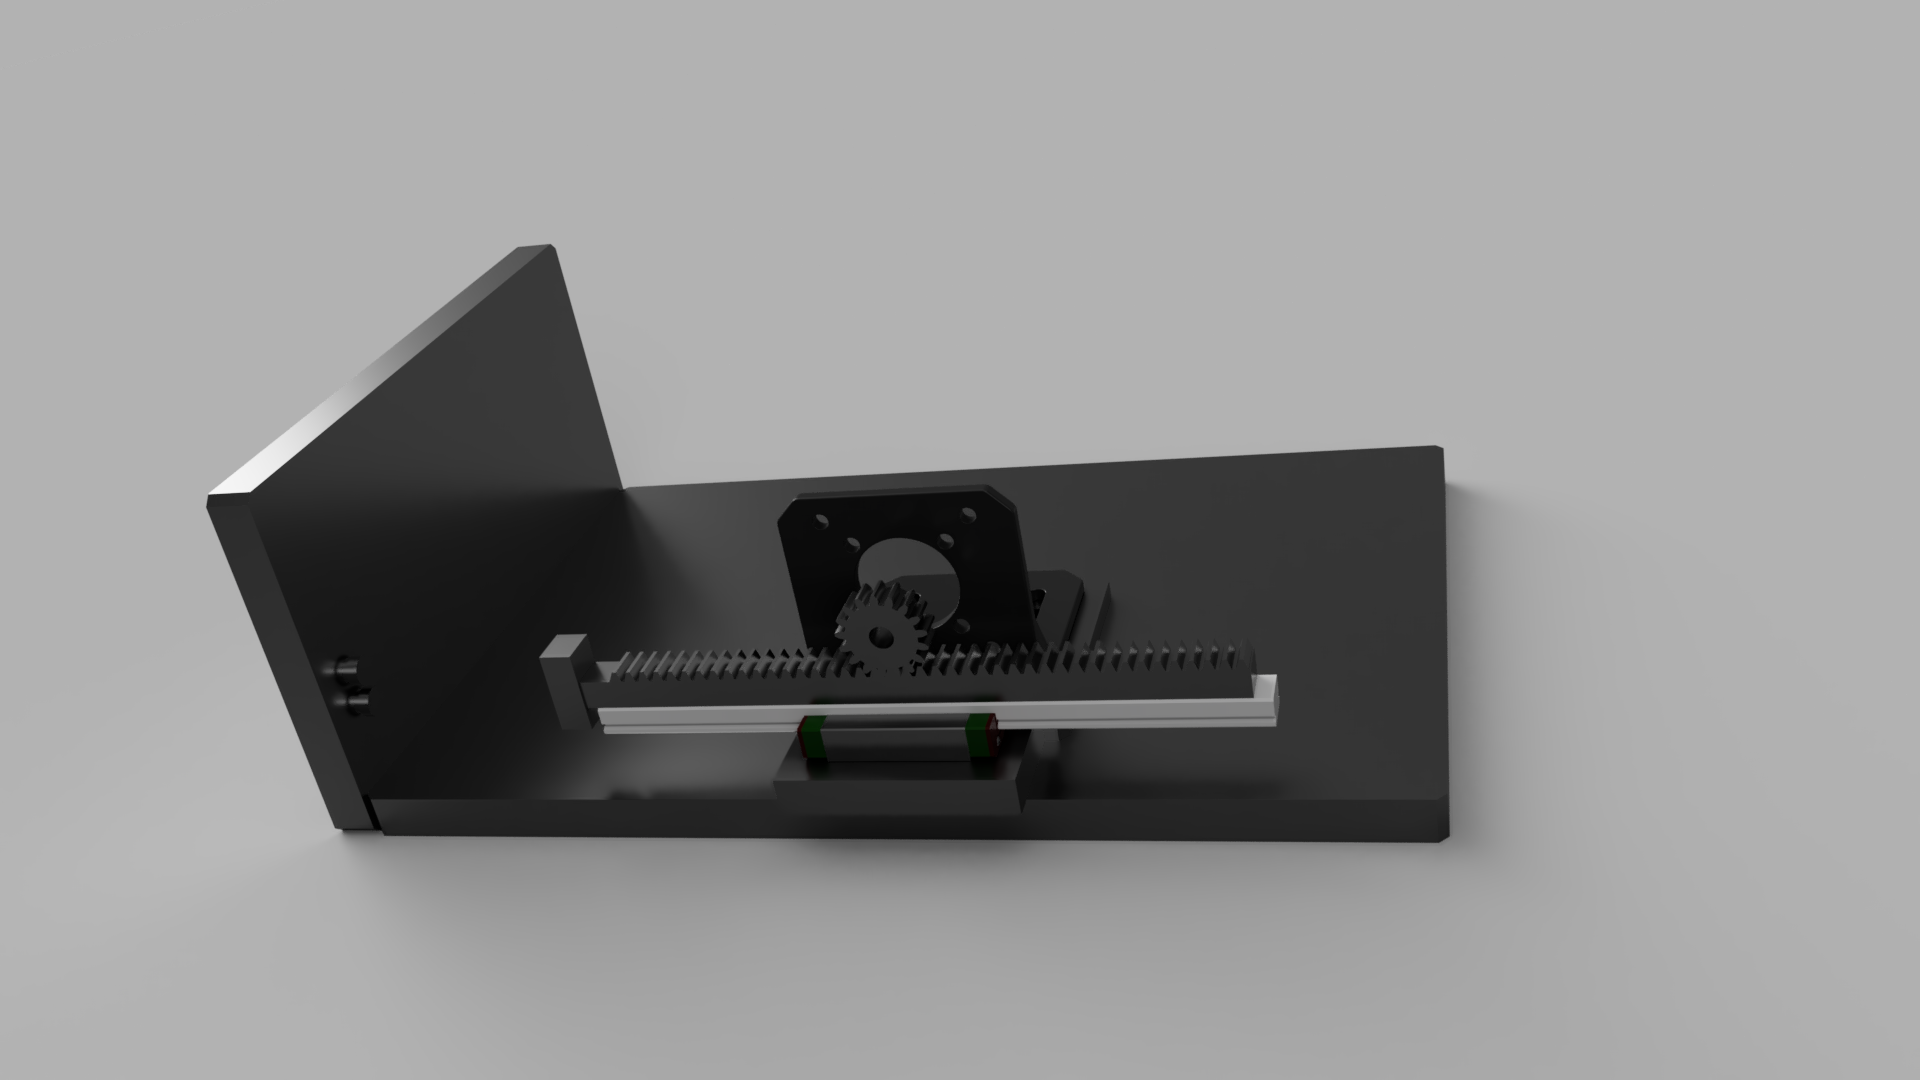
\includegraphics[width=1\linewidth]{Abbildung/dopple_feder_teststand_2026-Sep-14_05-20-54PM-000_CustomizedView4746332256.png}
    \caption{Enter Caption}
    \label{fig:Teststand}
\end{figure}
Dieses Projekt dient der Steuerung eines Endeffektors eines Roboterarms. Zuvor mussten wir jedoch die Steuerungs- und Simulationsfähigkeiten der von uns ausgewählten Komponenten und des Designs überprüfen und testen.
Aus diesem Grund wurde ein Prüfstand erstellt, um die Funktionalität des Greifers nachzubilden.

Der Prüfstand ermöglicht den Abgleich der berechneten Werte mit bekannten Parametern (Federn).

Mechanischer Aufbau
Der Prüfstand misst 240 × 85 × 150 mm. Der Motor ist auf einer Halterung montiert, die wiederum auf der Grundplatte befestigt ist.

\begin{table}
    \centering
    \begin{tabular}{|c|c|c|}\hline
         Pos.&  Komponente& Anmerkung\\\hline
         1&  Stepper motor 17HE12-1204S& seitlich an der Halterung befestigt\\\hline
 2& Motorhalterung&\\\hline
         3&  Ritzel m=1 z=17& auf der Motorwelle\\\hline
         4&  Zahnstange m =1 110mm& mit dem Ritzel verbunden\\\hline
         5&  Führungsschiene MGN9R& reist mit dem Zahnstange\\\hline
 6& Führungswagen MGN9H&an der Grundplatte befestigt\\\hline
         7&  Zwei Druckfedern mit jeweils 1,06 N/mm& am Ende der Zahnstange befestigt\\ \hline
    \end{tabular}
    
    
\end{table}
Der Schlitten, auf dem die Kugellager gelagert sind, ist an der Grundplatte befestigt, während Schiene und Zahnstange miteinander verbunden sind und sich gemeinsam bewegen. Die Schiene ist Teil der beweglichen Masse und dominiert diese (4.2). Der mechanische Hub beträgt etwa 95 mm.

Die beiden Druckfedern sind übereinander angeordnet und werden durch die Anschlagwand zusammengedrückt. Da beide die gleiche Verschiebung erfahren, addieren sich ihre Kräfte.

\textbackslash{}textbf\{Einschränkung:\} Die Motorhalterung besteht aus PLA. Aufgrund der hohen Temperatur des Motors bei längerem Betrieb kann sich die Halterung verformen. Innerhalb des Projektzeitrahmens stand kein anderes Material zur Verfügung. Für Testläufe von wenigen Sekunden Dauer ist dies unkritisch, für den Dauerbetrieb sollte die Halterung jedoch aus einem hitzebeständigeren Material bestehen.

Montage des Encoders
Der AS5600 wird an der Rückseite des Motors über eine Halterung befestigt, die den richtigen Abstand zum an der Welle angebrachten Magneten (2 mm) gewährleistet.

% +++++++++++++++++++++++++++++++++++++++++++++++++++++++++++++++++
% Schaltplan
% +++++++++++++++++++++++++++++++++++++++++++++++++++++++++++++++++
\section{Entwickelter Schaltplan}
\textit{Bearbeitet von Lars Hellriegel}\\

Abbildung~\ref{fig:Schaltplan} zeigt den Schaltplan des Prüfstands. Kernstück ist das \textit{Nucleo-F767ZI}-Board (STM32F767ZI), das über USB (ST-Link) mit einem Computer verbunden ist und sowohl die Regelung als auch die Kommunikation mit den Peripheriekomponenten übernimmt.

Die Positionserfassung erfolgt über einen \textit{AS5600}-Magnetfeld-Winkelsensor, der per I\textsuperscript{2}C (SCL/SDA) an die Pins PB8/PB9 des Nucleo-Boards angebunden ist. Die I\textsuperscript{2}C-Leitungen sind über zwei $4{,}7\,\mathrm{k\Omega}$-Widerstände nach 3,3\,V gegen Masse gepullt. Versorgt wird der Sensor mit 3,3\,V aus dem Nucleo-Board.

Die Ansteuerung des Schrittmotors erfolgt über einen \textit{TMC2209-v2.0}-Motortreiber. Dieser wird über die Steuersignale \texttt{STEP} (PE9), \texttt{DIR} (PE11) und \texttt{EN} (PE13) mit dem Microcontroller verbunden. Über PD5 ist zusätzlich eine UART-Diagnoseschnittstelle (\texttt{PDN\_UART}) realisiert, deren Leitung mit einem $1\,\mathrm{k\Omega}$-Widerstand als Pull-up/Strombegrenzung beschaltet ist. Die Leistungsversorgung des Treibers (\texttt{VM}) erfolgt über eine externe 12\,V-Quelle, die mit einem $1000\,\mathrm{\mu F}$-Kondensator gepuffert ist. Am Ausgang des Treibers (\texttt{M1A/M1B}, \texttt{M2A/M2B}) ist ein bipolarer Schrittmotor vom Typ \textit{NEMA17} mit seinen beiden Wicklungen (A+/A-, B+/B-) angeschlossen.

Die digitale Logik (Microcontroller, AS5600, Treiberlogik) wird mit 3,3\,V versorgt, während die Motorleistung über den separaten 12\,V-Kreis bereitgestellt wird. Die Masse (GND) ist für alle Teilsysteme gemeinsam geführt.

\begin{figure} [h]
    \centering
    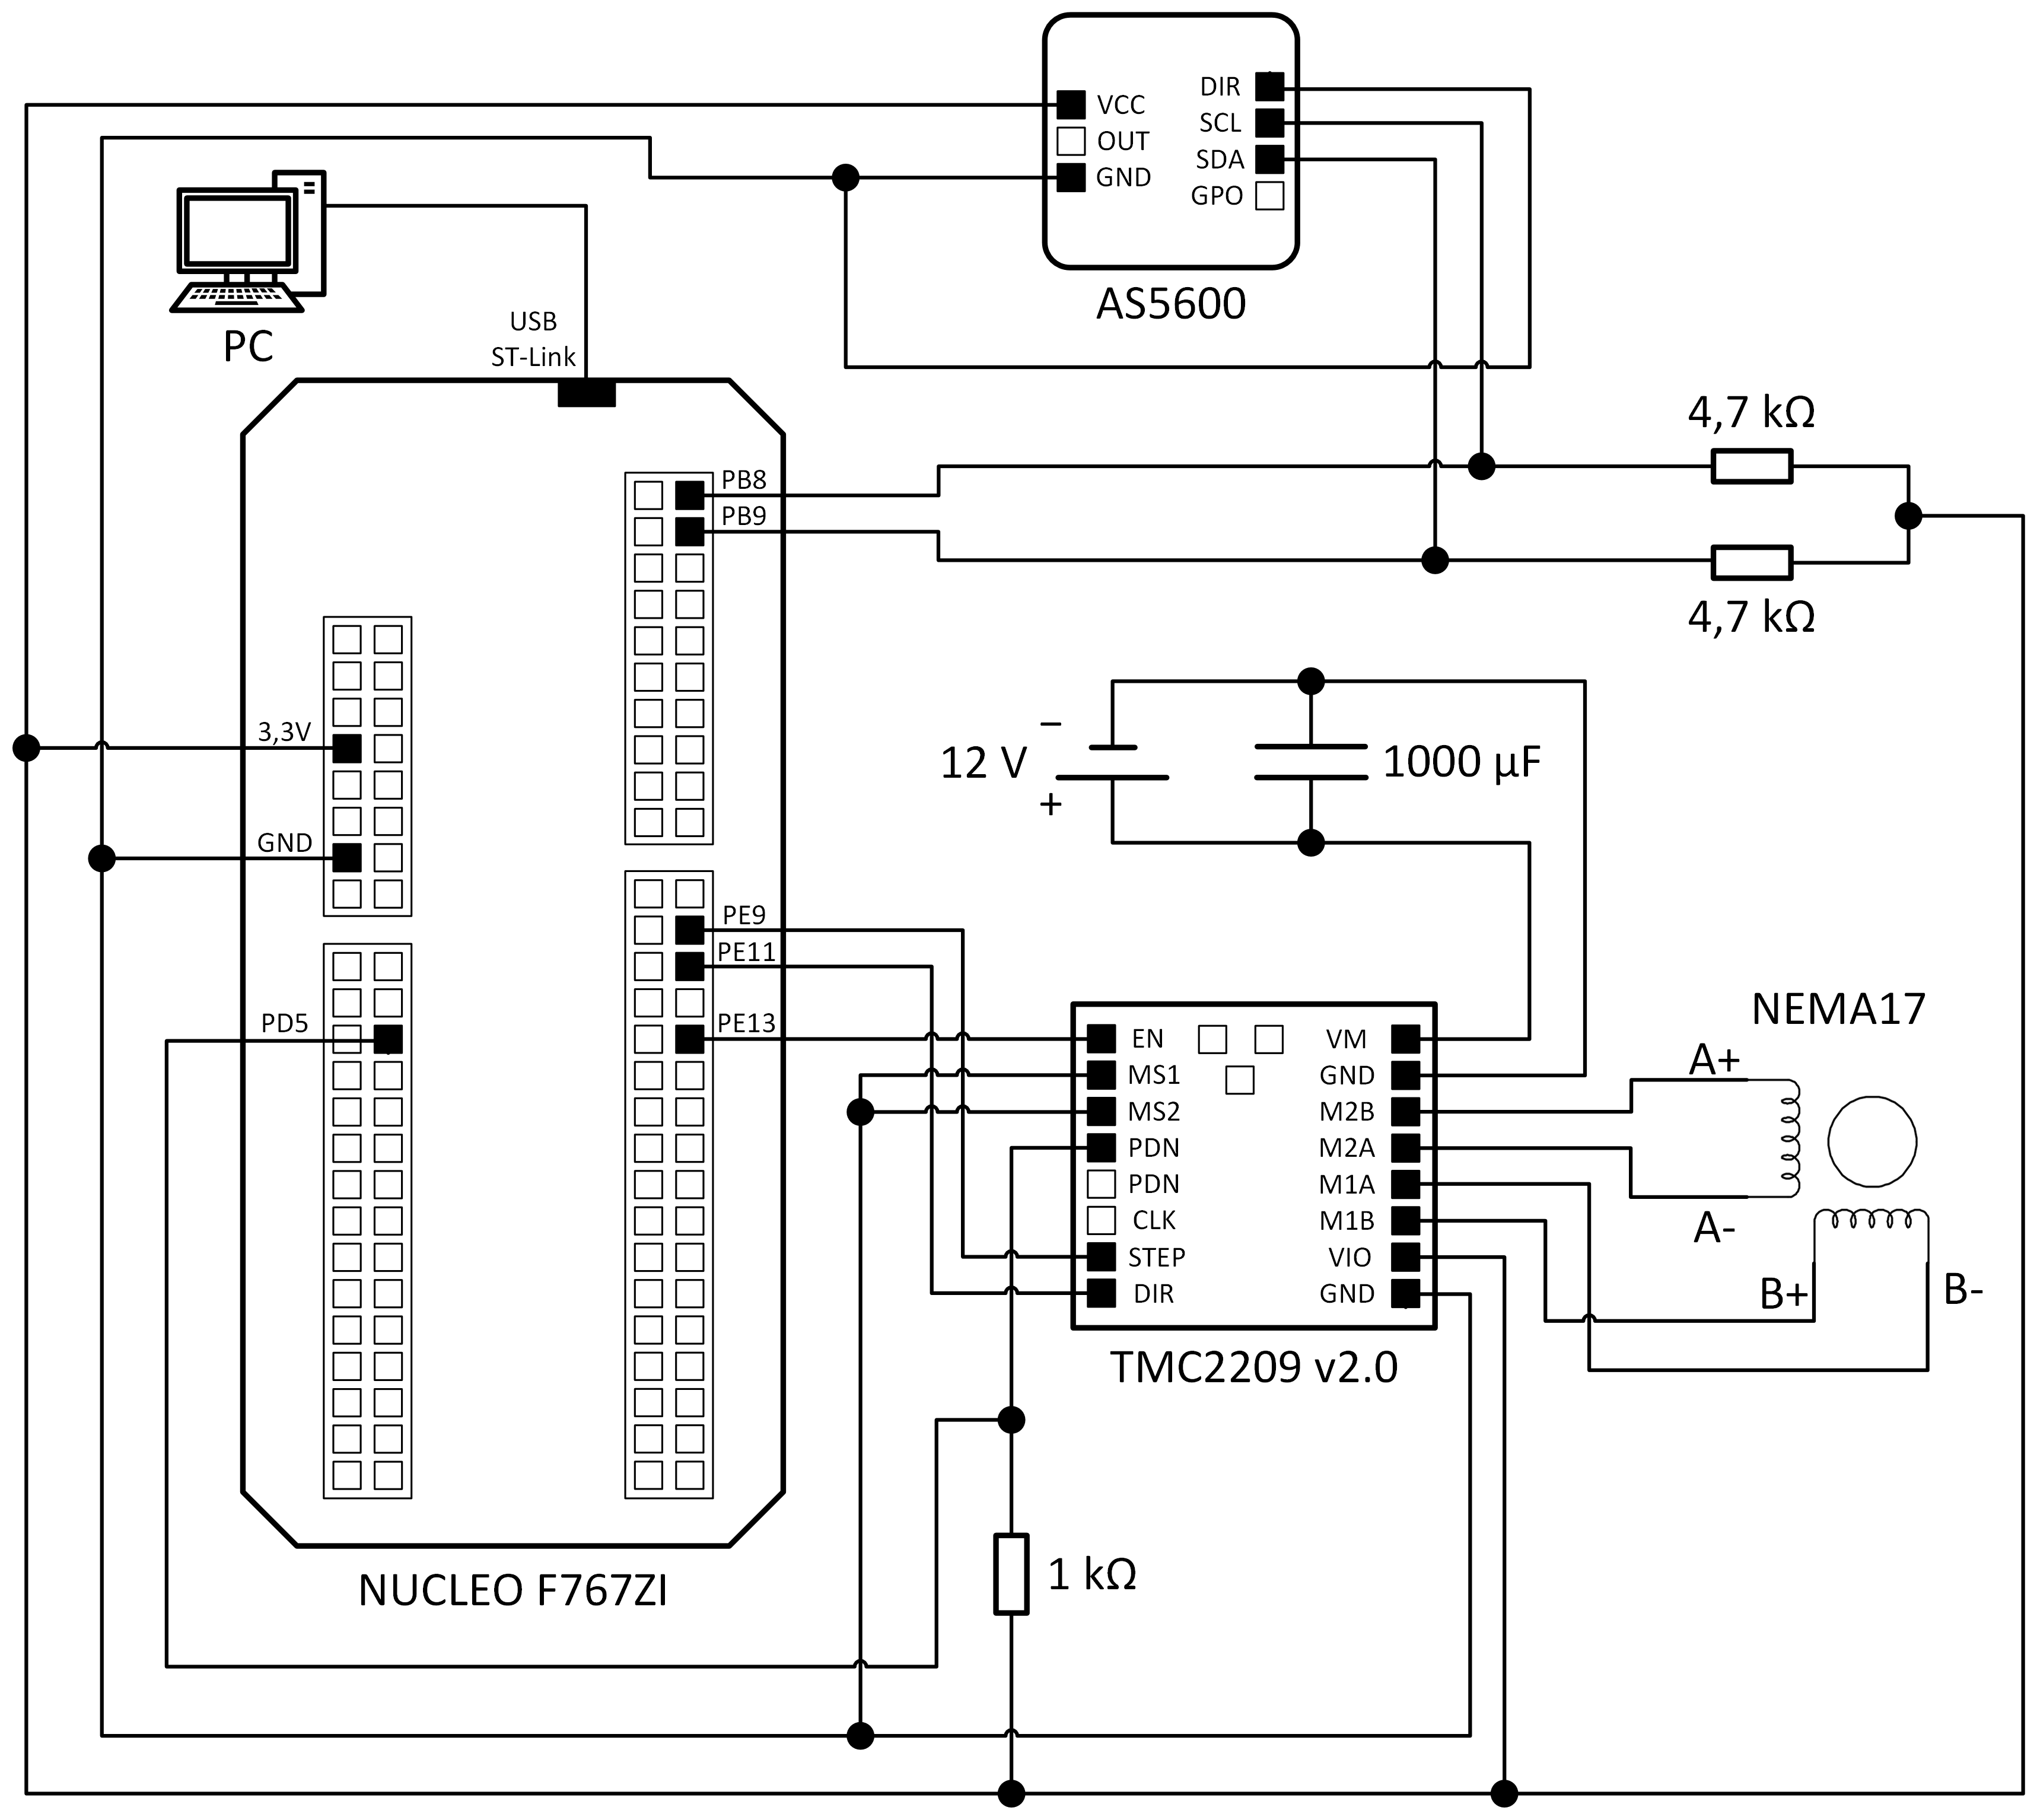
\includegraphics[width=1\linewidth]{Abbildung/SimReg_Schaltplan.png}
    \caption{Schaltplan des Prüfstands}
    \label{fig:Schaltplan}
\end{figure}



% \chapter{Systemcharakterisierung}\label{Charakterisierung}
% \section{Mechanik und Motorkennlinien}
% % Analyse von Übersetzung, Reibung, Spiel sowie Motor-/Treiberkennlinien.
% \textit{[Analyse der Mechanik und der Motor-/Treiberkennlinien]}
% \section{Systemgrenzen}
% % Ermittlung von max. Strom, Drehmoment, Geschwindigkeit.
% \textit{[Ermittelte Systemgrenzen: max. Strom, Drehmoment, Geschwindigkeit]}
% \section{Mathematisches Modell}
% % Vereinfachtes mathematisches Modell als Grundlage für den Reglerentwurf.
% \textit{[Herleitung des vereinfachten mathematischen Modells]}
\bigskip

% ---------------------------------------------------------
% Erfassung des Motorfeedbacks
% ---------------------------------------------------------
\chapter{Erfassung des Motorfeedbacks}\label{Kap:Feedback}


\textit{Bearbeitet von Mohammad Badr Eddin}\\

Für die Positionsregelung des Greifers ist eine zuverlässige Rückführung
der Position der Motorwelle erforderlich. Hierfür wird ein magnetischer
Positionssensor eingesetzt, der die Drehstellung der Welle berührungslos
erfasst. Das erfasste Feedback wird anschließend an den Mikrocontroller
übertragen und für die Positionsregelung verwendet.

\section{Positionsrückführung mit dem AS5600}
\label{sec:encoder}

Für die Erfassung der Motorposition wird ein magnetischer
Drehpositionssensor des Typs AS5600 eingesetzt. Der Sensor arbeitet
berührungslos und bestimmt die Winkelstellung eines Permanentmagneten,
der auf der Motorwelle angebracht ist. Dadurch kann die Position der
Motorwelle erfasst werden, ohne dass eine mechanische Verbindung
zwischen Sensor und Magnet erforderlich ist.

Der AS5600 besitzt eine interne 12-Bit-Auswertung und kann die
Winkelstellung über einen Bereich von $0^\circ$ bis $360^\circ$
erfassen. Damit eignet sich der Sensor für die Rückführung der
Motorposition innerhalb des Greiferantriebs. Der Sensor wird
nicht direkt zur Messung der linearen Fingerposition verwendet.
Stattdessen wird zunächst die Drehbewegung der Motorwelle erfasst und
die daraus resultierende lineare Bewegung des Greifers später über die
Kinematik des Zahnstangen-Ritzel-Systems bestimmt.


\subsection{Funktionsprinzip des magnetischen Sensors}

Die Winkelmessung des AS5600 basiert auf dem Hall-Effekt. Hierzu wird
ein Permanentmagnet so angeordnet, dass sich das Magnetfeld im Bereich
des Sensors mit der Drehung der Motorwelle verändert. Der AS5600
erfasst dieses Magnetfeld berührungslos und bestimmt daraus die
Winkelstellung des Magneten.

Für die vorgesehene Anwendung wird ein diametral magnetisierter
Permanentmagnet verwendet. Bei einer Drehung der Motorwelle dreht sich
der Magnet entsprechend mit. Die dadurch entstehende Änderung der
Magnetfeldrichtung wird vom Sensor erfasst und intern in einen
Winkelwert umgerechnet.

Die interne Auflösung des Sensors beträgt 12 Bit. Der vollständige
Messbereich wird dadurch in $4096$ diskrete Positionen unterteilt. Die
Winkelauflösung pro Messschritt beträgt somit

\begin{equation}
\Delta\varphi
=
\frac{360^\circ}{4096}
\approx 0{,}0879^\circ.
\end{equation}

Der ausgegebene Winkelwert stellt somit eine absolute Position
innerhalb einer Umdrehung dar. Eine Erfassung mehrerer Umdrehungen
erfolgt nicht direkt durch den Sensor, sondern kann bei Bedarf durch
eine entsprechende Verarbeitung der aufeinanderfolgenden Messwerte
in der Firmware realisiert werden.

\subsection{Mechanische Integration in den Greifer}
\label{sec:encoder_montage}

Der AS5600 ist an der Rückseite des Antriebs angeordnet. Der
Permanentmagnet wurde auf der hinteren Motorwelle befestigt und dreht
sich somit gemeinsam mit der Welle. Zur Befestigung wurde der Magnet
mit Schnellkleber auf der Rückseite der Welle fixiert. Der AS5600
selbst wurde über eine separate Halterung gegenüber dem Magneten
befestigt.

Für eine zuverlässige Winkelmessung ist die Positionierung des
Magneten gegenüber dem Sensor entscheidend. Der Magnet muss
korrekt zum Sensor ausgerichtet sein und sich im vorgesehenen
Messbereich des AS5600 befinden. Die Halterung sorgt dafür, dass der Sensor gegenüber dem Magneten in der vorgesehenen Position bleibt.


% \textit{Bearbeitet von Mohammad Badr Eddin}\\

% Für die Positionsregelung des Greifers ist eine zuverlässige Rückführung der Motorwelleposition erforderlich. Dazu wird die aktuelle Stellung des Antriebs über einen magnetischen Positionssensor erfasst und dem Mikrocontroller zur Verarbeitung bereitgestellt.
% Die erfasste Feedback ist in dem Fall eine Eingangsgröße für die Positionsregelung. 

% \section{Positionsrückführung mit dem AS5600}
% \label{sec:encoder}

% Für die Erfassung der Motorposition wird ein magnetischer
% Drehpositionssensor des Typs AS5600 eingesetzt. Der Sensor arbeitet
% kontaktlos und bestimmt die Winkelposition eines diametral magnetisierten
% Permanentmagneten. Die interne Auswertung gibt eine absolute
% Winkelposition mit einer Auflösung von 12 Bit über einen Bereich von
% $0^\circ$ bis $360^\circ$ aus.

% Der Sensor ist über die I\textsuperscript{2}C-Schnittstelle mit dem
% STM32F767 verbunden. Der AS5600 besitzt die 7-Bit-I\textsuperscript{2}C-
% Adresse $0x36$. Für die Positionsrückführung werden die
% Register \texttt{RAW\_ANGLE} bei den Adressen $0x0C$ und $0x0D$ verwendet.
% Diese liefern den 12-Bit-Rohwert der gemessenen Winkelposition. Zusätzlich
% wird das Statusregister bei Adresse $0x0B$ zur Erkennung des Magneten
% ausgewertet \cite{AMS}.

% \subsection{Auslesen des Encoderwertes}

% Die Firmware initialisiert den Encoder durch eine I\textsuperscript{2}C-
% Geräteerkennung. Anschließend wird der Rohwert zyklisch über einen
% Speicher-Lesezugriff aus den beiden \texttt{RAW\_ANGLE}-Registern
% ausgelesen. Die beiden Bytes werden zu einem 12-Bit-Wert zusammengesetzt:

% \begin{equation}
% N_{\mathrm{enc}}
% =
% \left(N_{\mathrm{high}} \ll 8\right)
% \mathbin{|}
% N_{\mathrm{low}}
% \end{equation}

% Anschließend werden die nicht verwendeten oberen Bits maskiert. Der
% resultierende Wertebereich beträgt somit

% \begin{equation}
% N_{\mathrm{enc}} \in [0,4095].
% \end{equation}

% Die Winkelauflösung des Sensors beträgt damit

% \begin{equation}
% \Delta\varphi
% =
% \frac{360^\circ}{4096}
% \approx 0{,}0879^\circ.
% \end{equation}


% \subsection{Umrechnung in die lineare Greiferposition}

% Für die Regelung wird nicht der Winkel des Encoders, sondern die daraus
% resultierende lineare Position des Greifers verwendet. Das Ritzel besitzt
% einen Teilkreisdurchmesser von $d=17\,\si{mm}$. Eine vollständige
% Umdrehung entspricht daher einer Umfangsstrecke von

% \begin{equation}
% s_{\mathrm{rev}}
% =
% \pi d
% =
% \pi \cdot 17\,\si{mm}
% \approx 53{,}41\,\si{mm}.
% \end{equation}

% Unter der Annahme einer direkten Kopplung zwischen Encoderwelle und Ritzel
% ergibt sich daraus die lineare Auflösung

% \begin{equation}
% \Delta x_{\mathrm{enc}}
% =
% \frac{s_{\mathrm{rev}}}{4096}
% =
% \frac{53{,}41\,\si{mm}}{4096}
% \approx 0{,}0130\,\si{mm}.
% \end{equation}

% Ein Encoder-Count entspricht somit etwa $\SI{13}{\micro\meter}$ linearer
% Bewegung am Ritzel.
% % +++++++++++++++++++++++++++++++++++++++++++++++++++++++++++++++++
% % Sensorik
% % +++++++++++++++++++++++++++++++++++++++++++++++++++++++++++++++++
% \section{Sensorik zur Strommessung}
% \textit{[Begründung Auswahl und Auswertung geeigneter Sensorik zur Strommessung]}


% % +++++++++++++++++++++++++++++++++++++++++++++++++++++++++++++++++
% % Signalaufbereitung
% % +++++++++++++++++++++++++++++++++++++++++++++++++++++++++++++++++
% \section{Signalaufbereitung}
% % Filterung, Skalierung der Rohdaten für die Regelung.
% \textit{[Filterung und Skalierung der Rohdaten für die Regelung]}
\bigskip


% ---------------------------------------------------------
% Reglerentwurf
% ---------------------------------------------------------
\chapter{Reglerentwurf}\label{Kap:Regler}
\textit{Bearbeitet von Masoud Fahim}\\

Die Aufgabenstellung sieht zwei Regler vor: einen Positionsregler für die Öffnungsweite
und einen Drehmomentregler für die Greifkraft. Der Positionsregler wurde wie vorgesehen
entworfen und umgesetzt. Für die Greifkraft wurde zunächst ein geschlossener Kraftkreis
über die StallGuard-Funktion des Treibers entworfen und simuliert; die Messungen am
Prüfstand zeigten jedoch, dass das Messglied die auftretende Last nicht auflöst. Die
Kraftaufgabe wird deshalb über den Positionsregler und die bekannte Federkennlinie
gesteuert. Dieses Kapitel beschreibt beide Wege, weil erst der verworfene Entwurf die
gewählte Lösung begründet.

% +++++++++++++++++++++++++++++++++++++++++++++++++++++++++++++++++
% Regelstrecke und Reglerstruktur
% +++++++++++++++++++++++++++++++++++++++++++++++++++++++++++++++++
\section{Regelstrecke und Wahl der Reglerstruktur}
\label{sec:strecke}

Der Motortreiber TMC2209 wird nicht über STEP/DIR, sondern über das Register
\texttt{VACTUAL} angesteuert. In dieser Betriebsart gibt der Mikrocontroller eine
Sollgeschwindigkeit vor, und der Treiber erzeugt die zugehörigen Mikroschritte
eigenständig mit einem internen Taktgenerator. Die Stellgröße des Regelkreises ist damit
eine Geschwindigkeit und keine Position.

Aus dieser Eigenschaft folgt die gesamte weitere Auslegung. Die Position der Zahnstange
ergibt sich als Zeitintegral der kommandierten Geschwindigkeit, die Regelstrecke ist also
ein reiner Integrator:

\begin{equation}
    G(s) = \frac{X(s)}{V(s)} = \frac{1}{s}
    \label{eq:strecke}
\end{equation}

Mit einem Proportionalregler $K_P$ lautet der offene Kreis

\begin{equation}
    L(s) = K_P \cdot G(s) = \frac{K_P}{s} ,
    \label{eq:offenerkreis}
\end{equation}

woraus sich die Durchtrittsfrequenz unmittelbar ablesen lässt. Der Betrag von $L(s)$
erreicht bei $\omega = K_P$ den Wert eins, sodass

\begin{equation}
    \omega_c = K_P
    \label{eq:durchtritt}
\end{equation}

gilt. Die Reglerverstärkung entspricht damit direkt der angestrebten Bandbreite des
geschlossenen Kreises, was die Parametrierung auf eine einzige Entwurfsentscheidung
reduziert.

\subsection*{Begründung der reinen P-Struktur}

Die Aufgabenstellung nennt eine Auslegung als PI-, PID- oder Zustandsregelung. Umgesetzt
wurde ein reiner P-Regler. Diese Abweichung ist keine Vereinfachung, sondern folgt
zwingend aus der Struktur der Strecke.

Der Integrator, der bei einer PI-Regelung üblicherweise im Regler ergänzt wird, um
bleibende Regelabweichungen zu vermeiden, ist hier bereits in der Strecke enthalten. Die
stationäre Genauigkeit ist deshalb ohne zusätzlichen I-Anteil gegeben: Damit die Position
im Beharrungszustand konstant bleibt, muss die kommandierte Geschwindigkeit null sein.
Wegen $v = K_P \cdot e$ ist das gleichbedeutend mit einer Regelabweichung von null. Ein
reiner P-Regler arbeitet an dieser Strecke also stationär exakt.

Ein zusätzlicher I-Anteil würde dagegen einen zweiten Integrator in den offenen Kreis
einbringen. Der Phasengang läge damit bereits ohne weitere Verzögerungen bei
$-180^\circ$, und die Stabilität des Kreises hinge allein von der Wahl der
Reglernullstelle ab. Der Regler wäre schwieriger zu parametrieren, ohne einen Vorteil bei
der Genauigkeit zu bieten.

Als Nebeneffekt entfällt eine sonst notwendige Anti-Windup-Maßnahme. Bei großen
Sollwertsprüngen arbeitet der Regler über den größten Teil der Fahrstrecke in der
Stellgrößenbegrenzung. Ein I-Anteil würde in dieser Zeit einen erheblichen Fehler
aufsummieren und nach Erreichen der Zielposition ein Überschwingen verursachen. Da kein
Integralanteil vorhanden ist, tritt dieser Effekt nicht auf, und die Begrenzung kann ohne
Zusatzlogik implementiert werden.

% +++++++++++++++++++++++++++++++++++++++++++++++++++++++++++++++++
% Positionsregler
% +++++++++++++++++++++++++++++++++++++++++++++++++++++++++++++++++
\section{Positionsregler}
\label{sec:positionsregler}

\subsection*{Wahl der Bandbreite}

Nach Gleichung \ref{eq:durchtritt} entspricht die Reglerverstärkung unmittelbar der
Bandbreite des geschlossenen Kreises. Die Auslegung reduziert sich damit auf die Frage,
wie schnell der Kreis sein soll. Als Zielbandbreite wurden $f_c = 20$~Hz gewählt, woraus

\begin{equation}
    K_P = 2\pi f_c = 2\pi \cdot 20\,\mathrm{Hz} = 125{,}7\,\mathrm{s^{-1}}
    \label{eq:kp}
\end{equation}

folgt. Der geschlossene Kreis verhält sich damit im linearen Bereich wie ein
Verzögerungsglied erster Ordnung mit der Zeitkonstante

\begin{equation}
    \tau = \frac{1}{K_P} = 7{,}96\,\mathrm{ms} .
    \label{eq:tau}
\end{equation}

Der Reglertask läuft mit einer Abtastzeit von $T = 2$~ms, entsprechend 500~Hz. Das
Produkt $K_P \cdot T = 0{,}251$ liegt deutlich unter eins, sodass der Kreis pro Abtastschritt
nur einen Bruchteil der verbleibenden Abweichung abbaut und die Diskretisierung das
Verhalten nicht dominiert.

\subsection*{Stellgrößenbegrenzung}

Die Geschwindigkeit wird auf $v_{max} = 40$~mm/s begrenzt. Dieser Wert ergibt sich aus der
zulässigen Motordrehzahl und entspricht einem Registerwert von \texttt{VACTUAL}~$= 3351$.

Der Begrenzung nachgeschaltet ist eine Anstiegsbegrenzung mit $a_{max} = 5000$~mm/s².
Sie ist kein optionales Komfortmerkmal: Der TMC2209 besitzt keinen Rampengenerator und
setzt eine sprunghaft geänderte Sollgeschwindigkeit unmittelbar um. Ohne softwareseitige
Begrenzung würde der Antrieb bei jedem Sollwertsprung mit einem Geschwindigkeitssprung
anfahren, was zu Schrittverlusten führen kann. Die Anstiegsbegrenzung übernimmt damit
die Funktion, die bei anderen Treibern in der Hardware liegt.

Der Zahlenwert ist nach unten begrenzt durch den Regler selbst. Bei einem Sollwertsprung
der Höhe $\Delta x$ ändert der Regler seine Ausgangsgröße mit
$\dot{v} = K_P^2 \cdot \Delta x$, bei einem Sprung von 0,2~mm also mit rund
3160~mm/s². Eine Anstiegsbegrenzung unterhalb dieses Wertes würde den Regler ausbremsen
und den Kreis verlangsamen, statt ihn zu schützen.

\subsection*{Totzone und Grenzzyklus}

Ohne weitere Maßnahme kommt der Antrieb im Stillstand nicht zur Ruhe. Ursache ist das
Verhältnis der beiden Auflösungen im Kreis. Ein Mikroschritt entspricht an der Zahnstange

\begin{equation}
    \Delta x_{\mu} = \frac{\pi \cdot d}{n_{voll} \cdot n_{\mu}}
    = \frac{\pi \cdot 17\,\mathrm{mm}}{200 \cdot 16} = 0{,}01669\,\mathrm{mm} ,
    \label{eq:mikroschritt}
\end{equation}

während eine Stufe des Encoders

\begin{equation}
    \Delta x_{enc} = \frac{\pi \cdot d}{2^{12}}
    = \frac{53{,}407\,\mathrm{mm}}{4096} = 0{,}01304\,\mathrm{mm}
    \label{eq:encoderstufe}
\end{equation}

beträgt. Der kleinstmögliche Stellschritt des Aktors ist damit um den Faktor 1,28 größer
als die kleinste auflösbare Messgröße. Der Motor kann folglich nicht auf einer
Encoderstufe zum Stehen kommen, sondern springt über sie hinweg. Der Regler erkennt die
entstandene Abweichung, korrigiert zurück, springt erneut darüber und so fort. Das
Ergebnis ist ein Grenzzyklus, der sich als dauerhaftes Pendeln der Geschwindigkeit um den
Nullpunkt äußert und am realen Antrieb als Brummen im Stillstand hörbar wird.

Abhilfe schafft eine Totzone unmittelbar hinter dem Summierer, die Abweichungen unterhalb
einer Schwelle nicht mehr korrigiert. Rechnerisch genügen dafür zwei Encoderstufen, also
0,026~mm. Am realen Aufbau erwies sich dieser Wert als zu klein: Die Herleitung
berücksichtigt ausschließlich die Quantisierung, nicht jedoch das Rauschen des
Messsignals. Die Totzone wurde deshalb auf 0,05~mm erhöht, was etwa vier Encoderstufen
entspricht. Erst mit diesem Wert geht die Geschwindigkeit im Stillstand auf null.

Die Totzone führt eine bleibende Positionsabweichung von bis zu 0,05~mm ein. Dieser
Kompromiss ist bewusst gewählt und nicht regelungstechnisch, sondern durch die Hardware
begründet: Feiner zu regeln, als der Aktor stellen kann, führt zwangsläufig zum
Grenzzyklus. Gegenüber der geforderten Positioniergenauigkeit von $\pm 0{,}5$~mm bleibt
ein Sicherheitsfaktor von zehn.

\subsection*{Aufbereitung des Messsignals}

Vereinzelt traten auf dem über I$^2$C gelesenen Encoderwert einzelne stark abweichende
Messwerte auf. Da der Regler proportional auf die Abweichung reagiert, würde ein solcher
Ausreißer unmittelbar in einen Geschwindigkeitssprung umgesetzt. Dem Encoderwert ist
deshalb ein Medianfilter über drei Werte nachgeschaltet. Er unterdrückt einzelne Spikes
vollständig, ohne die Dynamik des Kreises nennenswert zu verzögern, da er im Gegensatz zu
einem Mittelwertfilter keine Glättung über mehrere gültige Messwerte vornimmt.

\subsection*{Stabilitätsgrenzen}

Der Entwurfswert von $K_P = 125{,}7\,\mathrm{s^{-1}}$ ist nach oben durch zwei Effekte
begrenzt, die im kontinuierlichen Modell nach Gleichung \ref{eq:strecke} nicht enthalten
sind.

Die Abtastung führt eine Grenze ein, oberhalb derer der diskrete Kreis instabil wird. Für
$K_P \cdot T > 1$ überschreitet der Kreis das Ziel innerhalb eines Takts, ab
$K_P \cdot T = 2$ läuft er auf. Bei $T = 2$~ms entspricht das einer Grenze von
$K_P = 1000\,\mathrm{s^{-1}}$.

Die zweite Grenze stammt aus der Motordynamik. Der Rotor folgt dem Statorfeld nicht starr,
sondern als Feder-Masse-System aus magnetischer Steifigkeit und Trägheit. Bei dessen
Eigenfrequenz $\omega_0$ trägt dieses Schwingungsglied zusätzlich $-90^\circ$ zur bereits
vorhandenen Phasendrehung des Integrators bei, sodass der Kreis dort auf der kritischen
Phasenlage liegt. Über die Stabilität entscheidet dann allein der Betrag, woraus sich

\begin{equation}
    K_{P,max} = 2 \zeta \omega_0
    \label{eq:resonanzgrenze}
\end{equation}

ergibt. Mit $\omega_0 = 628\,\mathrm{rad/s}$ liefert diese Bedingung je nach Dämpfung
sehr unterschiedliche Werte, wie Tabelle \ref{tab:stabilitaetsgrenzen} zeigt.

% ---------------------------------------------------------------
\begin{table}[htbp]
    \centering
    \caption{Grenzen für $K_P$ aus Abtastung und Motorresonanz}
    \label{tab:stabilitaetsgrenzen}
    \begin{tabular}{lcc}
        \hline
        Ursache & Grenze für $K_P$ & Reserve zum Entwurfswert \\
        \hline
        Abtastung, $T = 2$~ms          & 1000 & Faktor 8 \\
        Motorresonanz, $\zeta = 0{,}20$ & 251  & Faktor 2 \\
        Motorresonanz, $\zeta = 0{,}10$ & 126  & keine \\
        \hline
    \end{tabular}
\end{table}
% ---------------------------------------------------------------

Die schärfere der beiden Bedingungen ist damit nicht die Abtastung, sondern die Resonanz.
Bemerkenswert ist der Fall $\zeta = 0{,}1$: Die verbreitete Faustregel, die Bandbreite
höchstens auf ein Fünftel der Resonanzfrequenz zu legen, ist rechnerisch identisch mit
Gleichung \ref{eq:resonanzgrenze} für genau diese Dämpfung. Die Faustregel unterstellt
also stillschweigend einen Zahlenwert, der im vorliegenden Fall nicht bekannt war.

Die Dämpfung wurde nicht messtechnisch bestimmt. Für die Inbetriebnahme wurde deshalb ein
reduzierter Startwert von $K_P = 100\,\mathrm{s^{-1}}$ vorgesehen. Der anschließende
Betrieb bei $K_P = 125{,}7\,\mathrm{s^{-1}}$ verlief ohne erkennbare Schwingneigung, was
nach Gleichung \ref{eq:resonanzgrenze} auf eine Dämpfung oberhalb von 0,1 schließen lässt.
Die Auslegung ist damit nachträglich abgesichert, ohne dass $\zeta$ als Zahlenwert
vorliegt.

\subsection*{Struktur des Regelkreises}

Abbildung \ref{fig:positionsregelkreis} fasst die beschriebenen Elemente zusammen.

% ---------------------------------------------------------------
\begin{figure}[htbp]
\centering
\begin{tikzpicture}[node distance=5mm,
    blk/.append style={text width=14mm}]

  \node (soll)                        {};
  \node[sum, right=8mm of soll] (s)   {$\pm$};
  \node[blk, right=6mm of s]    (dz)  {Totzone\\[-1pt]\tiny 0,05\,mm};
  \node[blk, right=3mm of dz]   (kp)  {$K_P$\\[-1pt]\tiny 125,7\,s$^{-1}$};
  \node[blk, right=3mm of kp]   (sat) {Sättigung\\[-1pt]\tiny $\pm$40\,mm/s};
  \node[blk, right=3mm of sat]  (rl)  {Rate Limiter\\[-1pt]\tiny 5000\,mm/s$^2$};
  \node[blk, right=3mm of rl]   (tmc) {Aktor\\[-1pt]\tiny TMC2209};
  \node[blk, right=3mm of tmc]  (int) {Integrator\\[-1pt]\tiny $1/s$};

  \coordinate[right=8mm of int] (tap);
  \node[right=1mm of tap, lbl] (xist) {$x$};

  \draw[sig] ($(soll)+(-6mm,0)$) -- node[lbl,above,pos=0.3]{$x_{soll}$} (s);
  \draw[sig] (s)   -- (dz);
  \draw[sig] (dz)  -- (kp);
  \draw[sig] (kp)  -- (sat);
  \draw[sig] (sat) -- (rl);
  \draw[sig] (rl)  -- (tmc);
  \draw[sig] (tmc) -- (int);
  \draw[line] (int) -- (tap);
  \fill (tap) circle (1.2pt);

  \node[lbl, above left=-1mm and -2mm of s]     {$+$};
  \node[lbl, below left=-1.5mm and -3.5mm of s] {$-$};

  \node[msg, below=16mm of $(kp)!0.5!(sat)$] (enc)
        {Messglied -- AS5600\\[-1pt]\tiny 0,01304\,mm je Count, Median-3};

  \draw[sig] (tap) |- (enc.east);
  \draw[sig] (enc.west) -| (s);

  \node[grp] at ($(dz.north)!0.5!(sat.north)+(0,4.5mm)$)  {Regler und Grenzen};
  \node[grp] at ($(tmc.north)!0.5!(int.north)+(0,4.5mm)$) {Aktor und Strecke};

\end{tikzpicture}
\caption{Blockschaltbild des Positionsregelkreises. Der Integrator ist Teil der
         Regelstrecke, nicht des Reglers.}
\label{fig:positionsregelkreis}
\end{figure}
% ---------------------------------------------------------------

Tabelle \ref{tab:reglerparameter} stellt die Parameter des Reglers zusammen.

% ---------------------------------------------------------------
\begin{table}[htbp]
    \centering
    \caption{Parameter des Positionsreglers}
    \label{tab:reglerparameter}
    \begin{tabular}{llp{6cm}}
        \hline
        Größe & Wert & Herkunft \\
        \hline
        $T$        & 2~ms                    & Periode des Reglertasks \\
        $K_P$      & 125,7~s$^{-1}$          & $2\pi \cdot 20$~Hz \\
        $v_{max}$  & 40~mm/s                 & zulässige Verfahrgeschwindigkeit \\
        $a_{max}$  & 5000~mm/s²              & oberhalb $K_P^2 \cdot \Delta x$ \\
        Totzone    & 0,05~mm                 & rund vier Encoderstufen \\
        \hline
    \end{tabular}
\end{table}
% ---------------------------------------------------------------

% +++++++++++++++++++++++++++++++++++++++++++++++++++++++++++++++++
% Kraftregelung über StallGuard - Entwurf
% +++++++++++++++++++++++++++++++++++++++++++++++++++++++++++++++++
\section{Kraftregelung über StallGuard}
\label{sec:sg_entwurf}

Für die Greifkraft war ursprünglich ein zweiter, geschlossener Regelkreis vorgesehen. Da
die Aufgabenstellung die zunächst angedachte Strommessung ausschließt und ein Kraftsensor
nicht vorhanden ist, bot sich die im Treiber bereits implementierte StallGuard-Funktion
als Messglied an. Dieser Abschnitt beschreibt den Entwurf. Die messtechnische
Überprüfung und die daraus folgende Verwerfung des Konzepts werden in Abschnitt
\ref{sec:sg_verwerfung} behandelt.

\subsection*{SG\_RESULT als Messgröße}

Der Rotor eines Schrittmotors ist ein Permanentmagnet und induziert bei Drehung eine
Spannung in den Statorwicklungen. Unter Last bleibt er weiter hinter dem umlaufenden
Statorfeld zurück, wodurch sich die Phasenlage dieser Spannung verschiebt. Der TMC2209
wertet diesen Zusammenhang intern aus und stellt das Ergebnis als Registerwert
\texttt{SG\_RESULT} bereit.

Entscheidend für den Reglerentwurf ist das Vorzeichen dieser Kennlinie. StallGuard wurde
zur Erkennung eines blockierten Motors entwickelt, der ausgegebene Wert läuft daher mit
steigender Last gegen null. Ein hoher Messwert bedeutet also eine geringe Belastung. Für
die Fehlerbildung folgt daraus

\begin{equation}
    e = \mathrm{SG_{ist}} - \mathrm{SG_{soll}} ,
    \label{eq:sg_fehler}
\end{equation}

also Ist minus Soll und damit genau umgekehrt zum Positionsregler. Wird diese Umkehrung
übersehen, ergibt sich ein selbsterhaltender Stillstand: Der Regler berechnet eine
negative Stellgröße, die von der Begrenzung auf null abgeschnitten wird, der Antrieb
bewegt sich nicht, und die Messgröße ändert sich folglich ebenfalls nicht.

\subsection*{Die Wandlungskette}

Anders als beim Positionsregler, bei dem der Encoder die Regelgröße unmittelbar misst,
liegt zwischen Stellgröße und Messgröße eine Kette physikalischer Umwandlungen. Jedes
Glied dieser Kette ist ein eigener Modellblock:

\begin{align}
    \Delta x &= \max(x - x_K,\; 0) \label{eq:kette_weg}\\
    F        &= c_{ers} \cdot \Delta x \label{eq:kette_kraft}\\
    M        &= 2 \cdot r \cdot F + M_{reib} \label{eq:kette_moment}\\
    \mathrm{SG} &= \mathrm{SG_0} - k_{SG} \cdot M \label{eq:kette_sg}
\end{align}

Gleichung \ref{eq:kette_weg} bildet den Kontakt ab. Die Begrenzung auf nichtnegative Werte
ist nicht rechentechnischer Natur, sondern physikalisch: Ein nachgiebiges Objekt kann
drücken, aber nicht ziehen. Solange der Finger den Kontaktpunkt $x_K$ nicht erreicht hat,
ist die Kraft exakt null.

Der Faktor zwei in Gleichung \ref{eq:kette_moment} berücksichtigt, dass das Ritzel beide
Zahnstangen gleichzeitig antreibt und sich die Momente beider Finger am Motor addieren.
Bei einem Wälzkreisradius von $r = 8{,}5$~mm entspricht damit jedes Newton Greifkraft je
Finger einem Motormoment von 17~Nmm. Das Reibmoment $M_{reib}$ liegt auch bei Leerfahrt
an und wird deshalb additiv berücksichtigt und nicht in den Kontaktblock gezogen.

Für die Zielkraft von 5~N je Finger ergibt sich daraus ein Nutzmoment von 85~Nmm,
zuzüglich eines geschätzten Reibmoments von 15~Nmm also rund 100~Nmm. Bezogen auf das
Haltemoment des Motors von etwa 260~Nmm entspricht das einer Auslastung von 38~Prozent.

\subsection*{Reglerstruktur}

Der Regler selbst entspricht strukturell dem Positionsregler: Proportionalglied,
Stellgrößenbegrenzung, Anstiegsbegrenzung. Die Verstärkung $K_v$ ist in mm/s je Zählschritt
angegeben.

Ein Unterschied betrifft die Stellgrößenbegrenzung. Ihre untere Grenze liegt nicht bei
$-v_{max}$, sondern bei null. Der Greifer soll während des Kraftaufbaus unter keinen
Umständen zurückfahren, da ein Richtungswechsel zunächst das Flankenspiel der Verzahnung
durchläuft und die aufgebrachte Kraft dabei schlagartig auf null fällt. Der Kraftaufbau
ist damit eine ausschließlich monotone Zustellbewegung.

Für die Verstärkung selbst existiert keine Auslegungsformel analog zu Gleichung
\ref{eq:kp}, da die Strecke in diesem Zweig keine geschlossene Übertragungsfunktion
besitzt. $K_v$ wurde deshalb so gewählt, dass die Zufahrgeschwindigkeit bei unbelastetem
Antrieb oberhalb der Gültigkeitsgrenze von \texttt{SG\_RESULT} liegt: Unterhalb von etwa
5~mm/s ist die induzierte Spannung zu klein und der Messwert wird zu Rauschen.

\subsection*{Strukturelle Grenze des Konzepts}

\texttt{SG\_RESULT} wird nicht zeitgetaktet aktualisiert, sondern einmal je Vollschritt,
also alle 0,267~mm Verfahrweg. Aus dieser Eigenschaft folgen zwei Einschränkungen, die
bereits im Entwurf erkennbar waren.

Zum einen hängt die Zahl der Messwerte, die während des Kraftaufbaus überhaupt anfallen,
ausschließlich von der Nachgiebigkeit des Objekts ab:

\begin{equation}
    N = \frac{F_{soll}}{c_{ers} \cdot \Delta x_{voll}}
    \label{eq:messwerte}
\end{equation}

Die Geschwindigkeit kürzt sich heraus. Langsameres Zufahren erhöht die Zahl der Messwerte
also nicht. Fordert man mindestens zehn Stützstellen zwischen Kontakt und Zielkraft, damit
von einer Regelung und nicht von einem Schwellwertschalter gesprochen werden kann, folgt
daraus die Auslegungsgrenze

\begin{equation}
    c_{ers} < \frac{F_{soll}}{10 \cdot \Delta x_{voll}} = 1{,}87\,\mathrm{N/mm} .
    \label{eq:steifigkeitsgrenze}
\end{equation}

Oberhalb dieser Steifigkeit springt die gemessene Kraft von einem zu kleinen auf einen zu
großen Wert, ohne dass ein Zwischenschritt existiert, an dem der Regler eingreifen könnte.

Zum anderen öffnet sich der Kreis genau dann, wenn er sein Ziel erreicht. Mit
verschwindender Geschwindigkeit wächst das Abtastintervall über alle Grenzen, und die
Rückführung friert auf dem zuletzt gemessenen Wert ein. Was danach geschieht -- Kriechen
des Materials, Temperaturdrift, ein Lastwechsel -- ist strukturell unsichtbar. Formal
handelt es sich damit nicht um eine Kraftregelung im Arbeitspunkt, sondern um eine
gesteuerte Zustellbewegung mit ereignisgetriggertem Abbruch.

Beide Einschränkungen wurden in der Simulation bestätigt und in der Auslegung
berücksichtigt. Sie waren jedoch nicht der Grund für die spätere Verwerfung des Konzepts;
diese beruht auf einem Befund am Messglied selbst, der sich erst am Prüfstand zeigte
(Abschnitt \ref{sec:sg_verwerfung}).

% +++++++++++++++++++++++++++++++++++++++++++++++++++++++++++++++++
% Kraftregelung über Position und Federmodell
% +++++++++++++++++++++++++++++++++++++++++++++++++++++++++++++++++
\section{Kraftvorgabe über Position und Federmodell}
\label{sec:kraft_position}

Nachdem sich \texttt{SG\_RESULT} als Messglied für die auftretende Last als ungeeignet
erwiesen hat, wurde die Kraftaufgabe auf einem anderen Weg gelöst. Grundlage ist die
Überlegung, dass bei bekannter Nachgiebigkeit des Objekts Kraft und Weg über das
Hookesche Gesetz eindeutig zusammenhängen. Eine Kraftvorgabe lässt sich damit in eine
Positionsvorgabe umrechnen und an den bereits vorhandenen, validierten Positionsregler
übergeben.

\subsection*{Prinzip}

Ein eigener Kraftregelkreis existiert nicht. Die Zielposition ergibt sich aus dem
Kontaktpunkt $x_0$ und dem für die gewünschte Kraft erforderlichen Federweg:

\begin{equation}
    x_{soll} = x_0 + \frac{F_{soll}}{c_{eff}}
    \label{eq:kraft_vorsteuerung}
\end{equation}

Die tatsächlich aufgebrachte Kraft folgt umgekehrt aus der gemessenen Position:

\begin{equation}
    F = c_{eff} \cdot (x_{ist} - x_0)
    \label{eq:kraft_rueckrechnung}
\end{equation}

Bezogen auf die Kraft ist dies ein offener Kreis: Sie wird berechnet, nicht gemessen. Der
darin eingebettete Positionskreis bleibt dagegen geschlossen und korrigiert jede
Abweichung der Position. Abbildung \ref{fig:gesamtstruktur} zeigt diese Schachtelung.

% ---------------------------------------------------------------
\begin{figure}[htbp]
\centering
\begin{tikzpicture}[node distance=5mm, scale=0.92, transform shape]

  \node (fin) {};
  \node[ghost, right=9mm of fin] (gs)  {$\pm$};
  \node[blk, right=7mm of gs]    (inv) {$1/c_{e\!f\!f}$\\[-1pt]\tiny 2,12\,N/mm};
  \node[blk, right=5mm of inv]   (x0)  {$+\,x_0$\\[-1pt]\tiny Kontaktpunkt};
  \node[blkw, right=14mm of x0, fill=black!6] (pos)
        {\textbf{Positionsregelkreis}\\[-1pt]\tiny geschlossen, Abb.~\ref{fig:positionsregelkreis}};
  \node[blkw, right=14mm of pos] (fed)
        {Feder (Strecke)\\[-1pt]\tiny $F=c_{e\!f\!f}(x-x_0)$};

  \coordinate[right=8mm of fed] (fout);
  \node[right=1mm of fout, lbl] {$F$};

  \draw[sig] ($(fin)+(-6mm,0)$) -- node[lbl,above,pos=0.3]{$F_{soll}$} (gs);
  \draw[sig] (gs)  -- (inv);
  \draw[sig] (inv) -- (x0);
  \draw[sig] (x0)  -- node[lbl,above=0.5mm]{$x_{soll}$} (pos);
  \draw[sig] (pos) -- node[lbl,above=0.5mm]{$x_{ist}$} (fed);
  \draw[line] (fed) -- (fout);
  \fill (fout) circle (1.2pt);

  \begin{scope}[on background layer]
    \node[draw, dashed, black!45, rounded corners=2pt,
          inner sep=2mm, fit=(pos)] (innen) {};
  \end{scope}
  \node[grp, above=1mm of innen] {geregelt};

  \draw[line, dashed, black!55] (fout) -- ++(0,-16mm) coordinate (fb2);
  \draw[line, dashed, black!55] (fb2) -| ($(gs)+(0,-16mm)$);
  \draw[miss] ($(gs)+(0,-16mm)$) -- (gs);

  \coordinate (xm) at ($(fb2)!0.55!($(gs)+(0,-16mm)$)$);
  \fill[white] ($(xm)+(-2mm,-2mm)$) rectangle ($(xm)+(2mm,2mm)$);
  \draw[red!60!black, line width=0.9pt]
        ($(xm)+(-1.6mm,-1.6mm)$) -- ($(xm)+(1.6mm,1.6mm)$);
  \draw[red!60!black, line width=0.9pt]
        ($(xm)+(-1.6mm,1.6mm)$) -- ($(xm)+(1.6mm,-1.6mm)$);
  \node[font=\scriptsize, text=red!60!black, below=1mm of xm]
        {keine Kraftrückführung};

\end{tikzpicture}
\caption{Gesamtstruktur der Kraftvorgabe. Der Positionsregelkreis bildet den
         geschlossenen Kern; der Kraftpfad darum herum ist offen. Die gestrichelte
         Linie markiert die Stelle, an der eine echte Kraftregelung ihre Rückführung
         hätte.}
\label{fig:gesamtstruktur}
\end{figure}
% ---------------------------------------------------------------

\subsection*{Ablauf eines Greifvorgangs}

Der Kontaktpunkt $x_0$ ist der einzige Parameter, der nicht aus der Auslegung stammt,
sondern im Versuch bestimmt werden muss. Der Ablauf gliedert sich daher in vier Schritte:

\begin{enumerate}
    \item Der Finger wird positionsgeregelt zugestellt, bis das Objekt gerade berührt wird.
    \item Die aktuelle Position wird als Kontaktpunkt $x_0$ übernommen.
    \item Die Zielposition wird nach Gleichung \ref{eq:kraft_vorsteuerung} berechnet und
          angefahren.
    \item Der Antrieb hält diese Position. Die Kraft steht.
\end{enumerate}

Die Übernahme von $x_0$ erfolgt derzeit manuell über die Bedienoberfläche. Eine
automatische Erkennung ist möglich, indem der Lastwinkel -- die Differenz zwischen dem
Schrittzähler des Treibers und der gemessenen Encoderposition -- ausgewertet wird. Dieser
liegt bei Leerfahrt praktisch bei null und springt bei Berührung auf einen messbaren Wert.

Für die Zielkraft von 5~N ergibt sich bei der am Prüfstand wirksamen Steifigkeit von
$c_{eff} = 2{,}12$~N/mm ein Federweg von 2,36~mm, bei 10~N entsprechend 4,72~mm.

\subsection*{Genauigkeit und Fehlerempfindlichkeit}

Da die Kraft nicht gemessen wird, geht jeder Fehler im Modell oder in der Position
unmittelbar und unkorrigiert in die Kraft ein. Die erreichbare Genauigkeit folgt damit
direkt aus der Positioniergenauigkeit. Mit der Totzone von 0,05~mm aus Abschnitt
\ref{sec:positionsregler} ergibt sich

\begin{equation}
    \Delta F = c_{eff} \cdot \Delta x = 2{,}12\,\mathrm{N/mm} \cdot 0{,}05\,\mathrm{mm}
    = 0{,}11\,\mathrm{N} .
    \label{eq:kraftfehler}
\end{equation}

Bemerkenswert ist das Skalierungsverhalten: Die \emph{absolute} Kraftgenauigkeit
verschlechtert sich linear mit der Steifigkeit. Bei einer einzelnen Feder mit 1,06~N/mm
läge der Fehler bei nur 0,05~N. Konstant bleibt lediglich der auf den Federweg bezogene
\emph{relative} Fehler, da sich der erforderliche Federweg umgekehrt proportional zu
$c_{eff}$ verhält. Daraus folgt unmittelbar die Anwendungsgrenze des Verfahrens: An einem
sehr steifen Objekt wird der Federweg so klein, dass die Positionsauflösung die Kraft
nicht mehr sinnvoll auflöst.

Ein Vergleich der drei Fehlerquellen zeigt, welche Größe die Genauigkeit tatsächlich
bestimmt. Da alle Zusammenhänge linear sind, lassen sich die Beiträge unmittelbar
angeben; eine Parameterstudie ist dafür nicht erforderlich.

% ---------------------------------------------------------------
\begin{table}[htbp]
    \centering
    \caption{Einfluss der Fehlerquellen auf die Greifkraft bei $F_{soll} = 5$~N und
             $c_{eff} = 2{,}12$~N/mm}
    \label{tab:fehlerquellen}
    \begin{tabular}{lcc}
        \hline
        Fehlerquelle & Kraftfehler & bezogen auf $F_{soll}$ \\
        \hline
        Totzone, $\pm 0{,}05$~mm          & $\pm 0{,}11$~N & 2,1~\% \\
        Kontaktpunkt $x_0$ um 0,5~mm falsch & 1,06~N        & 21,2~\% \\
        $c_{eff}$ um 5~\% falsch           & 0,25~N        & 5,0~\% \\
        \hline
    \end{tabular}
\end{table}
% ---------------------------------------------------------------

Die Bestimmung des Kontaktpunkts ist damit die kritische Größe des Verfahrens. Ein Fehler
von einem halben Millimeter, wie er bei manueller Zustellung ohne weitere Hilfsmittel
durchaus auftreten kann, wirkt sich zehnmal stärker aus als die gesamte
Positionierungenauigkeit des Reglers. Die Güte der Kraftvorgabe hängt folglich weniger am
Regler als an der Reproduzierbarkeit des Kontaktpunkts und an der Kenntnis der
Steifigkeit.

\subsection*{Einordnung}

Formal handelt es sich bei dem beschriebenen Verfahren um eine \emph{modellbasierte
Vorsteuerung mit geregelter Position} und nicht um eine Kraftregelung. Die Unterscheidung
ist nicht nur begrifflich, sondern bestimmt, welche Störungen ausgeregelt werden und
welche nicht:

\begin{itemize}
    \item \textbf{Keine Rückführung der Kraft.} Alles, was nach dem Anfahren der
          Zielposition geschieht -- Kriechen des Materials, Temperaturdrift, ein
          Lastwechsel am Objekt -- bleibt unbemerkt.
    \item \textbf{Die Steifigkeit muss bekannt sein.} An einem unbekannten Objekt ist das
          Verfahren nicht anwendbar, ohne $c_{eff}$ vorher zu bestimmen.
    \item \textbf{Der Kontaktpunkt geht direkt in die Kraft ein.} Er ist kein
          Auslegungsparameter, sondern muss bei jedem Greifvorgang neu ermittelt werden.
\end{itemize}

Diesen Einschränkungen steht gegenüber, dass das Verfahren ohne zusätzliche Sensorik
auskommt, auf einem bereits validierten Regelkreis aufsetzt und die geforderte
Umschaltung zwischen Positions- und Kraftbetrieb strukturell trivial macht: Beide
Betriebsarten nutzen denselben Regler und unterscheiden sich lediglich in der Herkunft
des Sollwerts. Die messtechnische Überprüfung erfolgt in Abschnitt
\ref{sec:ergebnis_kraft}.

% +++++++++++++++++++++++++++++++++++++++++++++++++++++++++++++++++
% Umschaltlogik und Zustandsautomat
% +++++++++++++++++++++++++++++++++++++++++++++++++++++++++++++++++
\section{Umschaltlogik und Zustandsautomat}
\label{sec:zustandsautomat}

Der Regler allein bildet nur einen Ausschnitt eines Greifvorgangs ab. Er berechnet aus
einer Abweichung eine Geschwindigkeit, weiß aber nicht, woher sein Sollwert stammt, ob
gerade referenziert, angenähert oder gegriffen wird und wie im Fehlerfall zu reagieren
ist. Diese Entscheidungen trifft eine übergeordnete Ablaufsteuerung, die als
Zustandsautomat im selben 2-ms-Task ausgeführt wird.

\subsection*{Zustände}

Die Ablaufsteuerung umfasst sechs Zustände. Tabelle \ref{tab:zustaende} fasst ihre
Aufgaben zusammen, Abbildung \ref{fig:zustandsautomat} zeigt die Übergänge.

% ---------------------------------------------------------------
\begin{table}[htbp]
    \centering
    \caption{Zustände der Ablaufsteuerung}
    \label{tab:zustaende}
    \begin{tabular}{llp{7.5cm}}
        \hline
        Zustand & Nr. & Aufgabe \\
        \hline
        \texttt{ST\_ZERO}      & 1 & Referenzfahrt, Nullpunkt setzen \\
        \texttt{ST\_DIRDETECT} & 2 & Bestimmung der Encoderrichtung \\
        \texttt{ST\_CONTROL}   & 3 & regulärer Regelbetrieb, Position oder Kraft \\
        \texttt{ST\_HOLD}      & 4 & Halten der erreichten Position bzw. Kraft \\
        \texttt{ST\_FAULT}     & 5 & Fehlerzustand, Motor gestoppt \\
        \texttt{ST\_OPEN}      & 6 & Öffnen und Lösen des Objekts \\
        \hline
    \end{tabular}
\end{table}
% ---------------------------------------------------------------

% ---------------------------------------------------------------
\begin{figure}[htbp]
\centering
\begin{tikzpicture}[x=1cm, y=1cm]

  \node[zst, fill=white] (idle) at (0,0)   {Idle\\[-1pt]\tiny nach dem Start};
  \node[zst]  (zero) at (3.4,0)            {\texttt{ST\_ZERO}\\[-1pt]\tiny Referenzfahrt};
  \node[zst]  (dir)  at (6.8,0)            {\texttt{ST\_DIRDETECT}\\[-1pt]\tiny Richtungs\-erkennung};
  \node[zst]  (ctrl) at (10.2,0)           {\texttt{ST\_CONTROL}\\[-1pt]\tiny Regelbetrieb};

  \node[zflt] (flt)  at (1.7,-2.4)         {\texttt{ST\_FAULT}\\[-1pt]\tiny Motor gestoppt};
  \node[zst]  (open) at (6.8,-2.4)         {\texttt{ST\_OPEN}\\[-1pt]\tiny Öffnen};
  \node[zst]  (hold) at (10.2,-2.4)        {\texttt{ST\_HOLD}\\[-1pt]\tiny Kraft halten};

  \draw[ztr] (idle) -- node[above]{Kommando}      (zero);
  \draw[ztr] (zero) -- node[above]{Nullpunkt}     (dir);
  \draw[ztr] (dir)  -- node[above]{Richtung}      (ctrl);
  \draw[ztr] (ctrl) -- node[right]{Ziel erreicht} (hold);
  \draw[ztr] (hold) -- node[below]{Kommando}      (open);
  \draw[ztr] (open.north east) -- node[above,pos=0.55,sloped]{fertig} (ctrl.south west);

  \draw[ztrd] (zero.south)     -- (flt.north east);
  \draw[ztrd] (dir.south west) -- (flt.north);
  \draw[ztrd] (open.west)      -- (flt.east);

  \node[grp, below=3mm of flt, text width=54mm, align=left]
        {gestrichelt: Fehlerbedingung. Sie führt aus \emph{jedem}
         Zustand nach \texttt{ST\_FAULT}; verlassen wird dieser nur
         durch einen Neustart.};

\end{tikzpicture}
\caption{Zustände und Übergänge der Ablaufsteuerung.}
\label{fig:zustandsautomat}
\end{figure}
% ---------------------------------------------------------------

\subsection*{Bestimmung der Encoderrichtung}

Der Zustand \texttt{ST\_DIRDETECT} verdient besondere Erwähnung, da er im ursprünglichen
Entwurf nicht vorgesehen war. Die Zuordnung zwischen der Zählrichtung des Encoders und
der Verfahrrichtung des Antriebs hängt davon ab, wie der Magnet auf der Welle sitzt und
wie der Sensor gegenüber der Mechanik orientiert ist. Sie ist aus der Konstruktion nicht
zuverlässig ableitbar.

Diese Zuordnung ist kein Randdetail. Bei falschem Vorzeichen wird aus der Gegenkopplung
des Regelkreises eine Mitkopplung: Die Regelabweichung wächst mit jedem Takt, der Regler
erhöht daraufhin die Geschwindigkeit weiter, und der Antrieb läuft weg, statt zu regeln.
Statt die Richtung als Konstante im Code festzulegen und bei einem Umbau auf einen Fehler
zu warten, wird sie beim Start experimentell bestimmt: Der Antrieb fährt mit einer kleinen,
festen Geschwindigkeit, und aus dem Vorzeichen der Encoderänderung wird die Zuordnung
abgeleitet.

\subsection*{Umschaltung zwischen den Betriebsarten}

Die Anforderung einer nahtlosen Umschaltung zwischen Positions- und Kraftbetrieb während
des laufenden Betriebs wird über die Variable \texttt{g\_ctrl\_mode} umgesetzt, die zur
Laufzeit über ein Bedienkommando geändert werden kann. Beide Betriebsarten laufen im
Zustand \texttt{ST\_CONTROL}.

Durch die in Abschnitt \ref{sec:kraft_position} gewählte Lösung ist diese Umschaltung
strukturell trivial. Da die Kraftvorgabe keinen eigenen Regelkreis besitzt, sondern
lediglich den Sollwert des Positionsreglers auf andere Weise berechnet, wird beim
Umschalten kein Regler getauscht. Es ändert sich ausschließlich die Herkunft von
$x_{soll}$: im Positionsbetrieb ein direkt vorgegebener Wert, im Kraftbetrieb das Ergebnis
von Gleichung \ref{eq:kraft_vorsteuerung}.

Damit entfallen sämtliche Probleme, die bei der Umschaltung zwischen zwei getrennten
Reglern zu behandeln wären: Es gibt keine Zustandsgrößen zu übergeben, keinen
stoßfreien Übergang zu konstruieren und keinen Sprung der Stellgröße im Umschaltmoment.
Die ursprünglich mit \texttt{SG\_RESULT} geplante Lösung hätte diesen Aufwand erfordert,
da dort ein zweiter Regler mit eigener Rückführung und eigener Fehlerbildung aktiv gewesen
wäre. Der Wegfall des zweiten Regelkreises ist an dieser Stelle kein Verlust, sondern eine
Vereinfachung.

\subsection*{Halten der Greifkraft}

Nach Erreichen der Zielposition geht die Ablaufsteuerung in den Zustand
\texttt{ST\_HOLD} über. Der Antrieb steht, muss aber weiterhin ein Moment aufbringen, da
die gespannte Feder ihn zurückzudrücken versucht.

Motortreiber reduzieren den Spulenstrom im Stillstand üblicherweise auf einen niedrigeren
Haltestrom, um die thermische Belastung zu senken. Der TMC2209 schaltet dazu nach Ablauf
der Zeit \texttt{TPOWERDOWN} von \texttt{IRUN} auf \texttt{IHOLD} um. Bei der hier
vorliegenden Anwendung führt dieses Verhalten jedoch dazu, dass das verbleibende
Haltemoment die anliegende Federkraft nicht mehr sicher aufnimmt. Die Folge wäre ein
Zurückdrücken des Antriebs und damit ein Einbruch der Greifkraft.

Aus diesem Grund wurde \texttt{IHOLD} dauerhaft auf denselben Wert wie \texttt{IRUN}
gesetzt. Gegenüber der ursprünglich vorgesehenen Umschaltung zur Laufzeit ist diese
Lösung einfacher und vermeidet einen weiteren Nebeneffekt: Die Kennlinie von
\texttt{SG\_RESULT} ist stromabhängig, sodass ein Wechsel des Stroms während des Betriebs
die Messwerte auf unterschiedliche Kennlinien legen würde. Erkauft wird dies mit einer
höheren Dauerverlustleistung im Stillstand, die bei den vorliegenden Strömen unkritisch
ist.

\subsection*{Fehlerverhalten}

Aus jedem Zustand führt eine Fehlerbedingung nach \texttt{ST\_FAULT}. Dort wird der Motor
angehalten, und weder Positions- noch Kraftvorgabe greifen weiterhin auf die
Motoransteuerung zu. Der Zustand kann nicht über ein reguläres Bedienkommando verlassen
werden; für eine erneute Inbetriebnahme ist ein bewusster Neustart erforderlich, nach dem
Referenzfahrt und Richtungserkennung erneut durchlaufen werden. Die einzelnen
Fehlerbedingungen und ihre Erkennung sind in Abschnitt \ref{sec:ueberlastschutz}
beschrieben.

\bigskip


% ---------------------------------------------------------
% Simulation
% ---------------------------------------------------------
\chapter{Simulation}\label{Kap:Simulation}
% =================================================================
% Kapitel: Simulation
% =================================================================

\textit{Bearbeitet von Masoud Fahim}\\

Die Aufgabenstellung sieht vor, die Reglerauslegung vor der praktischen Umsetzung zu
simulieren. Die Simulation erfüllt dabei zwei Zwecke: Sie dient zunächst der Überprüfung
der Auslegung gegen die theoretische Erwartung und liefert anschließend die
Vergleichsgrundlage, an der sich die Messungen am Prüfstand beurteilen lassen. Die
Modellbildung erfolgte in MATLAB Simulink.

% +++++++++++++++++++++++++++++++++++++++++++++++++++++++++++++++++
% Modellaufbau und Vorgehen
% +++++++++++++++++++++++++++++++++++++++++++++++++++++++++++++++++
\section{Modellaufbau und Vorgehen}
\label{sec:modellaufbau}

\subsection*{Schrittweiser Aufbau}

Das Modell wurde nicht in einem Zug erstellt, sondern in einzelnen Ausbaustufen. Jede
Stufe fügt genau einen Effekt hinzu, und für jede Stufe wurde vor dem Simulationslauf eine
Erwartung berechnet, gegen die das Ergebnis geprüft wurde.

Dieses Vorgehen ist aufwendiger als der unmittelbare Aufbau des vollständigen Modells,
hat aber einen entscheidenden Vorteil. Das Modell enthält mehrere Nichtlinearitäten --
Stellgrößenbegrenzung, Anstiegsbegrenzung, Quantisierung, Totzone -- die sich im Ergebnis
überlagern. Werden sie gemeinsam eingebaut und weicht das Ergebnis von der Erwartung ab,
lässt sich die Ursache nicht mehr einem einzelnen Block zuordnen. Wird dagegen jeweils nur
ein Effekt ergänzt, ist im Fehlerfall unmittelbar klar, welcher Block dafür verantwortlich
ist.

Ein Beispiel aus dem Aufbau verdeutlicht das: Die Anstiegsbegrenzung war zunächst auf
500~mm/s² gesetzt. Das Modell zeigte daraufhin ein deutliches Überschwingen mit
anschließendem Pendeln. Da in diesem Schritt ausschließlich die Stellgrößengrenzen
ergänzt worden waren, war die Ursache eindeutig zuzuordnen und der Wert konnte korrigiert
werden, bevor die nachfolgenden Effekte den Befund überdeckten. Die Begründung des
korrigierten Werts findet sich in Abschnitt \ref{sec:positionsregler}.

Als Referenz für die erste Stufe diente jeweils eine analytisch berechenbare Größe, etwa
die Sprungantwort eines Verzögerungsglieds erster Ordnung. Erst wenn diese im Modell
reproduziert wurde, kam der nächste Effekt hinzu.

\subsection*{Zentrale Parameterverwaltung}

Sämtliche Zahlenwerte des Modells sind in einem MATLAB-Skript \texttt{params.m}
hinterlegt, das vor jedem Simulationslauf ausgeführt wird. Die Simulink-Blöcke enthalten
keine numerischen Werte, sondern ausschließlich Variablennamen.

Diese Trennung hat sich aus zwei Gründen bewährt. Zum einen ist eine Größe, die an
mehreren Stellen im Modell auftritt -- etwa die Abtastzeit, die sowohl im Halteglied als
auch in der Anstiegsbegrenzung wirksam wird -- nur an einer Stelle zu ändern. Zum anderen
werden dieselben Werte auch von den Auswerteskripten verwendet, die Simulation und
Messung gegenüberstellen, sodass beide Seiten des Vergleichs zwangsläufig mit identischen
Parametern arbeiten.

Zusätzlich ist jeder Parameter mit einer Kennzeichnung seiner Herkunft versehen. Tabelle
\ref{tab:parameterstatus} erläutert die verwendeten Kürzel.

% ---------------------------------------------------------------
\begin{table}[htbp]
    \centering
    \caption{Kennzeichnung der Parameterherkunft in \texttt{params.m}}
    \label{tab:parameterstatus}
    \begin{tabular}{clp{8cm}}
        \hline
        Kürzel & Bedeutung & Beispiel \\
        \hline
        {[M]} & gemessen  & Federkonstante, Mikroschritteinstellung des Treibers \\
        {[B]} & berechnet & Weg je Mikroschritt, Encoderauflösung, $K_P$ \\
        {[A]} & Annahme   & Dämpfung, Totzeit, Kennlinie von \texttt{SG\_RESULT} \\
        \hline
    \end{tabular}
\end{table}
% ---------------------------------------------------------------

Die Unterscheidung ist nicht nur dokumentarischer Natur. Sie macht sichtbar, auf welchen
Annahmen eine Aussage des Modells beruht, und damit auch, wie belastbar diese Aussage
ist. Ein Modell, dessen Ergebnis von einem als [A] gekennzeichneten Parameter abhängt,
ist nur so gut wie diese Annahme. Wie sich im weiteren Verlauf zeigte, war genau das der
entscheidende Punkt bei der Bewertung des Kraftzweigs.

\subsection*{Umfang der Modelle}

Im Rahmen der Arbeit entstanden zwei Modelle. Das erste bildet den Positionsregelkreis ab
und wurde gegen Messdaten validiert. Das zweite bildete den geplanten Kraftregelkreis über
\texttt{SG\_RESULT} ab; es wurde nach der Verwerfung des Konzepts nicht weiterentwickelt,
ist aber als Beleg für die durchgeführte Auslegung dokumentiert. An seine Stelle trat eine
Erweiterung des Positionsmodells um die Federkennlinie. Die folgenden Abschnitte behandeln
die drei Modelle in dieser Reihenfolge.

% +++++++++++++++++++++++++++++++++++++++++++++++++++++++++++++++++
% Positionsregelkreis
% +++++++++++++++++++++++++++++++++++++++++++++++++++++++++++++++++
\section{Positionsregelkreis}
\label{sec:sim_position}

Das Modell des Positionsregelkreises entstand in sechs Stufen. Die Blockstruktur
entspricht dem in Abbildung \ref{fig:positionsregelkreis} gezeigten Regelkreis; Abbildung
\ref{fig:simulink_position} zeigt die Umsetzung in Simulink.

% ---------------------------------------------------------------
\begin{figure}[htbp]
    \centering
    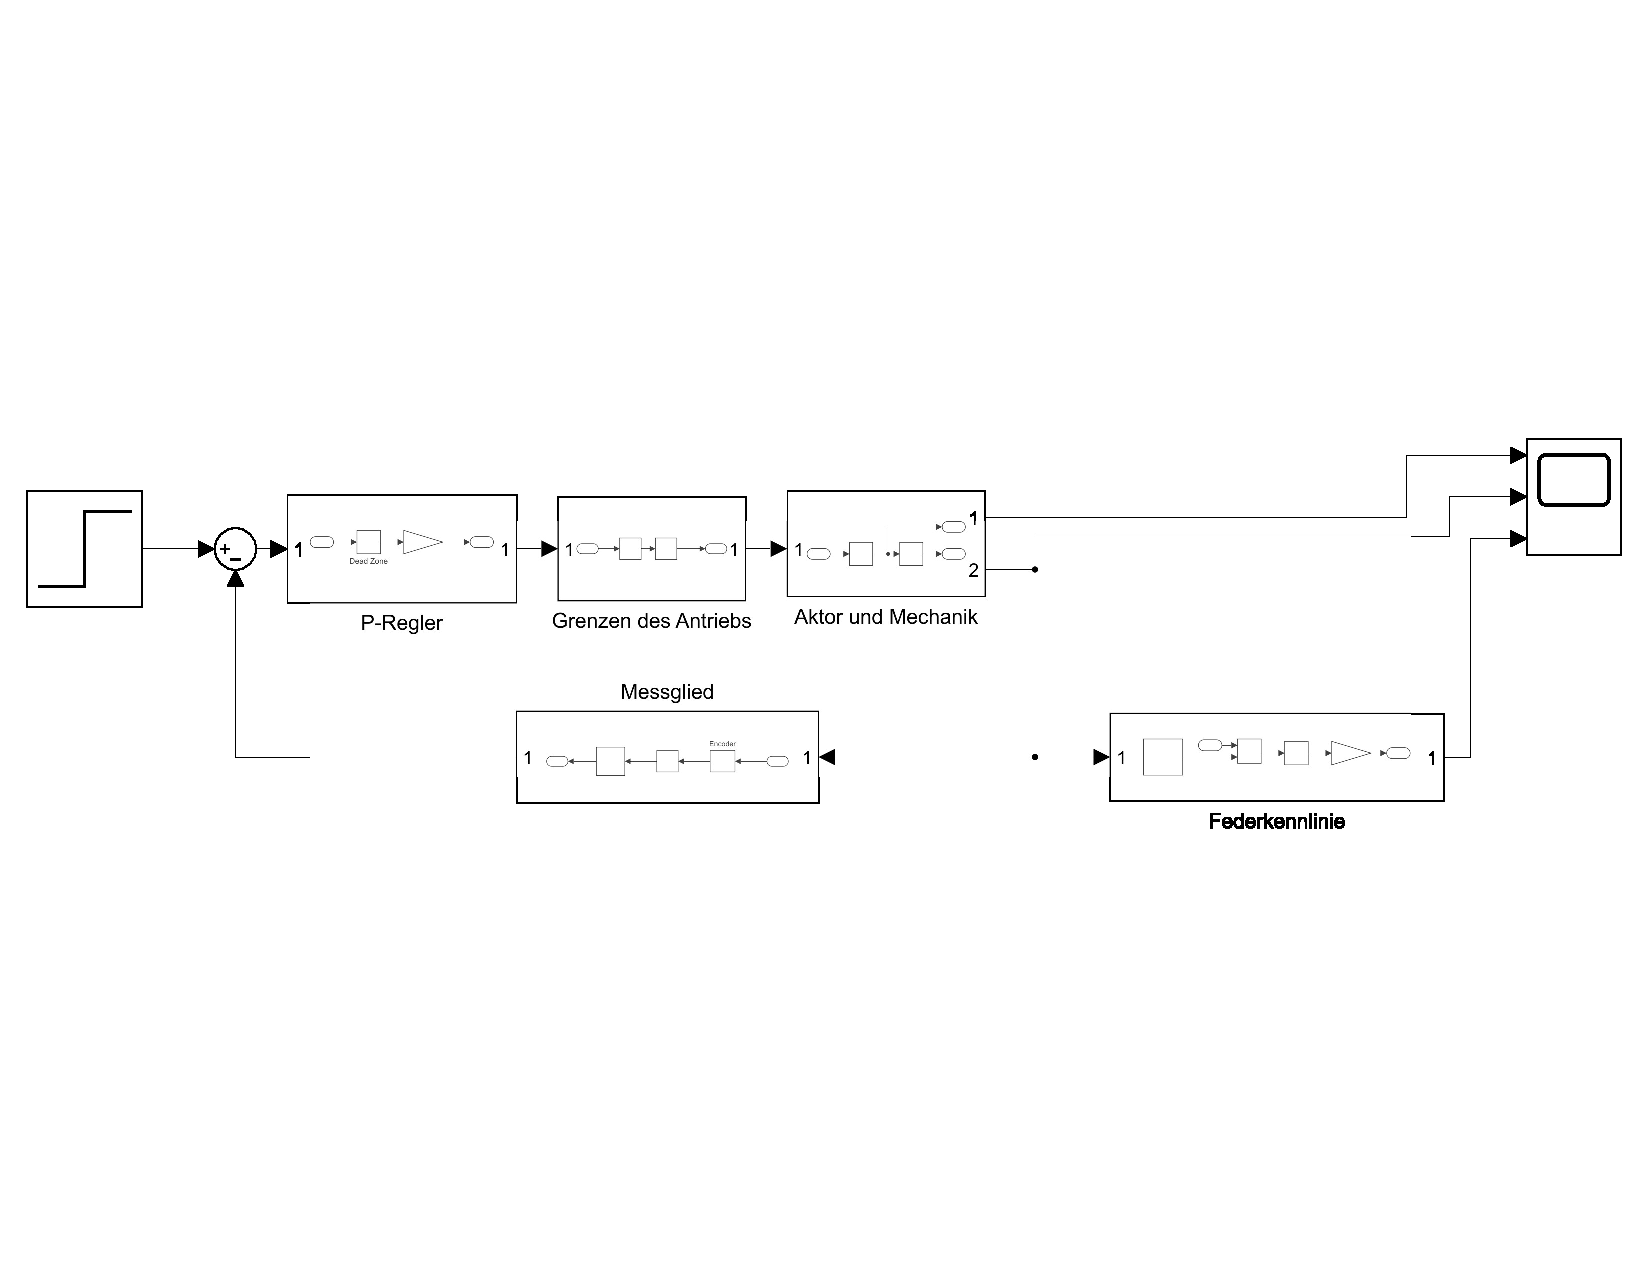
\includegraphics[width=\textwidth, trim=12pt 205pt 13pt 200pt, clip]
                    {Abbildung/Positions_Effort_Regelkreis.pdf}
    \caption{Simulink-Modell des Positionsregelkreises. Die obere Reihe bildet Regler,
             Stellgrößengrenzen sowie Aktor und Strecke ab, der linke untere Zweig das
             Messglied. Der rechte untere Zweig \texttt{Federkennlinie} berechnet die
             Kraft aus der Position und ist nicht Teil des Regelkreises
             (Abschnitt \ref{sec:sim_feder}).}
    \label{fig:simulink_position}
\end{figure}
% ---------------------------------------------------------------

\subsection*{Stufe 1: Idealmodell}

Die erste Stufe besteht aus fünf Blöcken: Sprungfunktion, Summierer, Verstärkung,
Integrator und Anzeige. Weder Abtastung noch Begrenzungen oder Quantisierung sind
enthalten. Der geschlossene Kreis entspricht damit exakt der Übertragungsfunktion

\begin{equation}
    G_w(s) = \frac{K_P}{s + K_P} ,
    \label{eq:fuehrung}
\end{equation}

also einem Verzögerungsglied erster Ordnung mit der Zeitkonstante $\tau = 1/K_P$. Als
Referenz diente der in MATLAB berechnete Verlauf von \texttt{step(tf(Kp,[1 Kp]))}.

Bei einer Sprunghöhe von 0,2~mm ergeben sich die in Tabelle \ref{tab:stufe1} genannten
Prüfpunkte. Alle drei wurden vom Modell getroffen.

% ---------------------------------------------------------------
\begin{table}[htbp]
    \centering
    \caption{Prüfpunkte des Idealmodells bei einem Sprung von 0,2~mm}
    \label{tab:stufe1}
    \begin{tabular}{llp{6cm}}
        \hline
        Zeitpunkt & Position & Bedeutung \\
        \hline
        $t = 7{,}96$~ms  & 0,1264~mm & 63,2~\%, entspricht $\tau$ \\
        $t = 23{,}9$~ms  & 0,1900~mm & 95~\%, entspricht $3\tau$ \\
        Endwert          & 0,2000~mm & keine bleibende Abweichung trotz reinem P-Anteil \\
        \hline
    \end{tabular}
\end{table}
% ---------------------------------------------------------------

Der Endwert bestätigt die in Abschnitt \ref{sec:strecke} gegebene Begründung der
P-Struktur: Obwohl der Regler keinen Integralanteil besitzt, verbleibt keine
Regelabweichung.

\subsection*{Stufe 2: Abtastung}

In der zweiten Stufe wurde ein Halteglied nullter Ordnung mit der Abtastzeit $T$ in den
Rückführzweig eingefügt. Es bildet ab, dass der Encoder nur alle 2~ms gelesen wird und
der Messwert bis zur nächsten Messung konstant bleibt. Der Kreis folgt damit der
Differenzengleichung

\begin{equation}
    x[k+1] = x[k] + K_P T \cdot \big(x_{soll} - x[k]\big) .
    \label{eq:diskret}
\end{equation}

Charakteristisch ist, dass das Verhältnis aufeinanderfolgender Geschwindigkeitsstufen
konstant bleibt und

\begin{equation}
    \frac{v[k+1]}{v[k]} = 1 - K_P T = 0{,}749
    \label{eq:polstelle}
\end{equation}

beträgt. Dieser Wert ist zugleich die Polstelle des diskreten Kreises und diente als
Prüfgröße: Im Modell ergab sich für die ersten Stufen ein Verhältnis von
$18{,}82 / 25{,}13 = 0{,}749$, in Übereinstimmung mit Gleichung \ref{eq:polstelle}.

Die Abtastung führt darüber hinaus eine Stabilitätsgrenze ein, die im kontinuierlichen
Modell der ersten Stufe nicht existiert. Bei $K_P T = 1$ erreicht der Kreis das Ziel
innerhalb eines Takts, darüber schwingt er alternierend, und ab $K_P T = 2$ läuft er auf.
Bei $T = 2$~ms entspricht das der in Tabelle \ref{tab:stabilitaetsgrenzen} genannten
Grenze von $K_P = 1000\,\mathrm{s^{-1}}$.

\subsection*{Stufe 3: Stellgrößengrenzen}

Die dritte Stufe ergänzt die Begrenzung auf $\pm v_{max}$ und die nachgeschaltete
Anstiegsbegrenzung. Die Sättigung greift, sobald die Regelabweichung den Wert

\begin{equation}
    e^{*} = \frac{v_{max}}{K_P} = \frac{40\,\mathrm{mm/s}}{125{,}7\,\mathrm{s^{-1}}}
    = 0{,}318\,\mathrm{mm}
    \label{eq:esat}
\end{equation}

überschreitet. Bei einem Sprung von 10~mm bedeutet das, dass der Antrieb über mehr als
99~\% der Fahrstrecke mit konstanter Höchstgeschwindigkeit fährt und sich das
exponentielle Verhalten des Reglers erst auf den letzten Zehntelmillimetern zeigt.

Daraus ergibt sich eine wichtige Konsequenz für die Verifikation: Zur Überprüfung von
$K_P$ sind ausschließlich Sprünge unterhalb von 0,3~mm geeignet. Bei größeren Sprüngen
misst man die Sättigungsgeschwindigkeit und erhält keinerlei Aussage über den Regler.
Beide Fälle wurden simuliert, da große Sprünge den realistischen Betriebsfall darstellen.

In dieser Stufe trat der bereits in Abschnitt \ref{sec:modellaufbau} erwähnte Fehler auf.
Die Anstiegsbegrenzung war zunächst auf 500~mm/s² gesetzt, was zu einem Überschwingen mit
anschließendem Pendeln führte. Ursache ist, dass der Regler seine Ausgangsgröße bei einem
Sprung der Höhe $\Delta x$ von sich aus mit

\begin{equation}
    \dot{v} = K_P^2 \cdot \Delta x
    \label{eq:reglerbeschleunigung}
\end{equation}

ändert, bei einem Sprung von 0,2~mm also mit rund 3160~mm/s². Eine Begrenzung unterhalb
dieses Werts bremst nicht den Antrieb, sondern den Regler. Mit 5000~mm/s² läuft der Kreis
sauber ein.

Als Nebenbefund bestätigte diese Stufe, dass trotz der langen Sättigungsphase kein Windup
auftritt. Ein PI-Regler hätte über die rund 0,24~s dauernde Sättigungsfahrt bei einem
10-mm-Sprung eine Regelabweichung von nahezu 10~mm aufintegriert und eine
Anti-Windup-Logik erfordert.

\subsection*{Stufe 4: Quantisierung}

Die vierte Stufe ergänzt zwei Quantisierer: einen im Rückführzweig für die Auflösung des
Encoders und einen vor dem Integrator für die Mikroschritte des Motors. Damit zeigt das
Modell den in Abschnitt \ref{sec:positionsregler} beschriebenen Grenzzyklus: Die
Geschwindigkeit wechselt dauerhaft zwischen kleinen positiven und negativen Werten,
anstatt auf null zu gehen.

Mit der Totzone hinter dem Summierer verschwindet dieses Verhalten, und die
Geschwindigkeit erreicht exakt null. Das Modell bestätigt damit sowohl die Ursache des
Effekts als auch die Wirksamkeit der gewählten Gegenmaßnahme.

\subsection*{Stufe 5: Totzeit}

Die fünfte Stufe ergänzt eine Totzeit im Rückführzweig, die das Lesen über I$^2$C und die
Rechenzeit im Task abbildet. Ihr Einfluss ist gegenüber der Abtastzeit von 2~ms gering;
die Phasenreserve sinkt um wenige Grad. Sichtbar wird der Effekt erst in der Nähe der
Stabilitätsgrenze und damit weit oberhalb des Entwurfswerts von $K_P$.

\subsection*{Stufe 6: Motorresonanz und Entscheidung gegen ihre Modellierung}

Die sechste Stufe sah ein Schwingungsglied zweiter Ordnung zwischen Integrator und
Abgriffpunkt vor. Es bildet ab, dass der Rotor der kommandierten Schrittfolge nicht starr
folgt, sondern als Feder-Masse-System aus magnetischer Steifigkeit und Trägheit. Diese
Stufe lieferte die in Abschnitt \ref{sec:positionsregler} diskutierte
Stabilitätsbedingung nach Gleichung \ref{eq:resonanzgrenze}.

Im finalen Modell ist dieses Glied nicht enthalten. Der Grund ist der Abgleich mit den
Messdaten: Das reine Integratormodell trifft den gemessenen Verlauf bereits im Rahmen der
Messgenauigkeit (Abschnitt \ref{sec:ergebnis_abgleich}). Eine Ergänzung des
Schwingungsglieds würde die Übereinstimmung nicht verbessern, hätte aber zwei freie
Parameter -- Eigenfrequenz und Dämpfung -- eingeführt, die beide nicht gemessen wurden.
Ein Modell mit unbestimmten Parametern, das keine bessere Übereinstimmung liefert, ist dem
einfacheren Modell nicht vorzuziehen.

Die Stabilitätsanalyse bleibt davon unberührt. Sie war als Auslegungsschritt notwendig,
um die zulässige Höhe von $K_P$ abzuschätzen, und führte zu der Entscheidung, die
Inbetriebnahme mit reduziertem Wert zu beginnen. Dass sich ihr Ergebnis im Betrieb als
unkritisch erwies, entwertet den Schritt nicht -- es begrenzt lediglich die Dämpfung des
realen Motors nach unten.

% +++++++++++++++++++++++++++++++++++++++++++++++++++++++++++++++++
% Kraftregelkreis über SG_RESULT
% +++++++++++++++++++++++++++++++++++++++++++++++++++++++++++++++++
\section{Kraftregelkreis über SG\_RESULT}
\label{sec:sim_sg}

Der in Abschnitt \ref{sec:sg_entwurf} beschriebene Kraftregelkreis wurde nach demselben
Verfahren aufgebaut wie der Positionskreis. Da die Wandlungskette zwischen Stellgröße und
Messgröße hier aus mehreren physikalischen Stufen besteht, entstand das Modell in sechs
Schritten entlang dieser Kette.

\subsection*{Aufbau entlang der Wandlungskette}

Die ersten vier Schritte bilden das Messglied ab, wobei als Eingangsgröße zunächst eine
Rampe als Platzhalter für den Antrieb diente. Erst im fünften Schritt wurde der Kreis
geschlossen.

\begin{description}
    \item[E1 -- Kontaktmodell] Federweg nach Gleichung \ref{eq:kette_weg} mit Begrenzung
          auf nichtnegative Werte, anschließend Multiplikation mit der Steifigkeit.
          Prüfpunkt: Vor dem Kontaktpunkt muss die Kraft exakt null sein und nicht
          negativ; bei doppeltem Federweg muss sich die Kraft verdoppeln.
    \item[E2 -- Momentbildung] Umrechnung der Kraft in ein Motormoment nach Gleichung
          \ref{eq:kette_moment}, anschließend Addition des Reibmoments. Prüfpunkt: vor
          dem Kontakt 15~Nmm, bei Sollkraft 100~Nmm. Dieser Schritt diente zugleich der
          Kontrolle des Faktors zwei -- eine Rechnung mit nur einer Zahnstange hätte
          57,5~Nmm ergeben.
    \item[E3 -- Kennlinie des Sensors] Fallende Gerade nach Gleichung \ref{eq:kette_sg},
          begrenzt auf den Registerbereich und quantisiert auf gerade Werte, da das
          niederwertigste Bit von \texttt{SG\_RESULT} fest null ist. Rechnerisch ergibt
          sich für die Sollkraft ein Wert von 285; im Modell erscheint 284, weil ein
          ungerader Zielwert im Register nicht existiert.
    \item[E4 -- Abtastung je Vollschritt] Quantisierung der Position auf das
          Vollschrittraster von 0,267~mm vor dem Kontaktblock. Damit springen Kraft,
          Moment und Messwert gemeinsam nur an den Vollschrittpositionen.
    \item[E5 -- Regler] Ergänzung von Fehlerbildung, Verstärkung, Begrenzungen und
          Integrator. Damit entfällt die Rampe, die Geschwindigkeit stammt nun aus dem
          Regler. Prüfpunkt: Bei Leerfahrt beträgt die Regelabweichung
          $382 - 284 = 98$~Zählschritte, die Zufahrgeschwindigkeit also 9,8~mm/s.
    \item[E6 -- Grenzfall] Derselbe Regler bei erhöhter Steifigkeit, siehe unten.
\end{description}

\subsection*{Die Auslegungsgrenze}

Schritt E4 liefert das wesentliche Ergebnis dieses Modells. Da der Messwert an das
Vollschrittraster gekoppelt ist, fällt während des Kraftaufbaus nur eine begrenzte Zahl
von Stützstellen an. Nach Gleichung \ref{eq:messwerte} ergeben sich bei einer Steifigkeit
von 1~N/mm rund 19 Messwerte. Diese Zahl wurde in der Simulation durch Abzählen der
Stufen bestätigt und ist der eigentliche Beleg für die Richtigkeit des Modellschritts.

Schritt E6 wiederholt denselben Lauf mit einer auf 10~N/mm erhöhten Steifigkeit.
Zwischen Kontakt und Zielkraft liegen dann nur noch zwei Messwerte. Der Regler misst am
ersten Vollschritt ein Moment von rund 60~Nmm und damit zu wenig, am zweiten bereits
106~Nmm und damit mehr als den Sollwert. Ein Zwischenschritt, an dem er die Geschwindigkeit
sinnvoll reduzieren könnte, existiert nicht.

Damit ist die in Gleichung \ref{eq:steifigkeitsgrenze} genannte Grenze von 1,87~N/mm nicht
nur hergeleitet, sondern simulativ belegt. Oberhalb dieser Steifigkeit degeneriert die
Regelung zu einem Schwellwertschalter mit einem einzigen Messwert Vorwarnung. Für den
Greifer folgte daraus, dass ein nachgiebiger Finger keine Nebensache ist, sondern die
Voraussetzung dafür, dass das Konzept überhaupt funktionieren kann.

\subsection*{Bewertung des Modells im Nachhinein}

Das Modell war strukturell korrekt. Die Wandlungskette, die Vorzeichenumkehr bei der
Fehlerbildung, die Quantisierung auf gerade Registerwerte und die Kopplung der Abtastung
an das Vollschrittraster bilden das reale Verhalten des Treibers zutreffend ab. Auch die
strukturelle Schwäche des Konzepts -- das Öffnen des Kreises bei verschwindender
Geschwindigkeit -- zeigte sich in der Simulation daran, dass die Endwerte nicht exakt auf
dem Sollwert stehen bleiben.

Dennoch traf das Modell in einem entscheidenden Punkt eine falsche Vorhersage. Es ging
von einer Ruhelage bei 382 Zählschritten und einem Abfall auf 284 unter Last aus,
während die Messung am Prüfstand einen über den gesamten Verfahrweg konstanten Wert von
etwa 33 ergab (Abschnitt \ref{sec:sg_verwerfung}).

Die Ursache liegt nicht in der Struktur, sondern in der Parametrierung. Die beiden Größen,
die die Kennlinie nach Gleichung \ref{eq:kette_sg} festlegen -- der Wert $\mathrm{SG_0}$
ohne Last und die Steigung $k_{SG}$ -- waren als Annahmen in den Parametersatz eingegangen
und in Tabelle \ref{tab:parameterstatus} entsprechend als [A] gekennzeichnet. Sie wurden
nie an der Hardware überprüft, weil eine solche Überprüfung einen lauffähigen Prüfstand
vorausgesetzt hätte, der zum Zeitpunkt der Modellbildung nicht existierte.

Die Simulation konnte damit zeigen, dass die \emph{Regelstruktur} bei einem Messglied mit
den angenommenen Eigenschaften funktionieren würde. Sie konnte nicht zeigen, ob das
Messglied diese Eigenschaften tatsächlich besitzt. Die Aussagekraft eines Modells ist
durch denjenigen seiner Parameter begrenzt, der am schlechtesten abgesichert ist -- und
das war hier nicht der Regler, sondern der Sensor.

Für die Arbeit hat dieser Befund methodischen Wert. Er begründet, warum die
Kennzeichnung der Parameterherkunft nach Tabelle \ref{tab:parameterstatus} kein
formaler Aufwand ist: Sie hätte bereits vor der Inbetriebnahme sichtbar gemacht, dass die
zentrale Aussage des Kraftmodells vollständig auf zwei ungeprüften Zahlenwerten ruht.

% +++++++++++++++++++++++++++++++++++++++++++++++++++++++++++++++++
% Federkennlinie als Nachlauf
% +++++++++++++++++++++++++++++++++++++++++++++++++++++++++++++++++
\section{Federkennlinie als Nachlauf}
\label{sec:sim_feder}

Nach der Verwerfung des Konzepts aus Abschnitt \ref{sec:sim_sg} stellte sich die Frage,
wie der Kraftzweig zu modellieren ist. Die Antwort folgt unmittelbar aus der in Abschnitt
\ref{sec:kraft_position} gewählten Lösung: Da kein Kraftregelkreis existiert, ist auch
kein zweites Modell erforderlich. Es genügt, das validierte Positionsmodell um die
Umrechnung von Position in Kraft zu erweitern.

\subsection*{Aufbau}

Das Subsystem \texttt{Federkennlinie} besteht aus drei Blöcken und enthält keine
Rückführung:

\begin{enumerate}
    \item Differenzbildung $x - x_0$ zur Bestimmung des Federwegs,
    \item Begrenzung auf nichtnegative Werte,
    \item Multiplikation mit der Steifigkeit $c_{eff}$.
\end{enumerate}

Die Begrenzung ist auch hier der eigentliche Kontakt: Solange der Finger den
Kontaktpunkt nicht erreicht hat, ist der Federweg negativ und die Kraft muss exakt null
sein. Eine Feder kann drücken, aber nicht ziehen. Ohne diese Begrenzung würde das Modell
vor dem Kontakt eine negative Kraft ausgeben, die physikalisch nicht existiert.

Der Abgriff des Positionssignals erfolgt am Ausgang der Strecke und damit vor dem
Messglied. Das ist keine Frage der Zeichnung, sondern inhaltlich bedeutsam: Die Feder wird
von der tatsächlichen Position der Zahnstange zusammengedrückt, nicht von dem Wert, den
der Encoder daraus macht. Ein Abgriff hinter dem Messglied würde die Quantisierung des
Encoders und dessen Totzeit fälschlich in die Kraft einrechnen.

Dass dieser Zweig strukturell kein Teil des Regelkreises ist, lässt sich am Modell in
Abbildung \ref{fig:simulink_position} unmittelbar ablesen: Er ist an denselben
Positionsausgang angeschlossen wie das Messglied, von seinem Ausgang führt jedoch kein
Signalweg zurück in den Kreis. Er bildet ausschließlich ab, welche Kraft sich aus der
ohnehin geregelten Position ergibt.

\subsection*{Erwarteter Kraftverlauf}

Der simulierte Greifvorgang verwendet dieselben Werte wie der Versuch am Prüfstand:
Kontaktpunkt $x_0$, Zielkraft 5~N und daraus nach Gleichung \ref{eq:kraft_vorsteuerung}
eine Zielposition von $x_0 + 2{,}36$~mm. Der Verlauf gliedert sich in drei Abschnitte,
die sich sämtlich vorab berechnen lassen und als Prüfpunkte dienten:

% ---------------------------------------------------------------
\begin{table}[htbp]
    \centering
    \caption{Prüfpunkte des simulierten Greifvorgangs, Zeit ab Kontakt}
    \label{tab:sim_kraft}
    \begin{tabular}{llp{7cm}}
        \hline
        Zeit ab Kontakt & Kraft & Vorgang \\
        \hline
        $< 0$                     & 0~N             & Zustellung mit $v_{max}$, kein Kontakt \\
        $0 \ldots 51$~ms          & 0 \ldots 4,33~N & Kraftaufbau bei konstanter Geschwindigkeit \\
        ab 51~ms                  & $\to 5{,}00$~N  & Regler verlässt die Sättigung, exponentielles Einlaufen \\
        \hline
    \end{tabular}
\end{table}
% ---------------------------------------------------------------

Das Ende der Sättigungsphase liegt dort, wo die verbleibende Regelabweichung den Wert
$e^{*}$ aus Gleichung \ref{eq:esat} unterschreitet, also 0,318~mm vor der Zielposition.
Bei $v_{max}$ entspricht das 51~ms nach dem Kontakt. Der Endwert wird nach weiteren
$3\tau$, also rund 75~ms nach dem Kontakt, praktisch erreicht.

\subsection*{Zur Form des Kraftverlaufs}

Der Anstieg zwischen Kontakt und Sättigungsende ist \emph{linear} und nicht
exponentiell. Ursache ist, dass der Regler in diesem gesamten Abschnitt in der
Stellgrößenbegrenzung arbeitet: Die Geschwindigkeit ist konstant, der Federweg wächst
daher linear mit der Zeit, und mit ihm die Kraft. Die Steigung beträgt

\begin{equation}
    \frac{\mathrm{d}F}{\mathrm{d}t} = c_{eff} \cdot v_{max}
    = 2{,}12\,\mathrm{N/mm} \cdot 40\,\mathrm{mm/s} = 84{,}8\,\mathrm{N/s} .
    \label{eq:kraftanstieg}
\end{equation}

Erst auf den letzten rund 0,3~mm zeigt sich die Dynamik des Reglers. Über 85~Prozent des
Kraftaufbaus sind damit keine Reglereigenschaft, sondern eine reine Zustellbewegung mit
Höchstgeschwindigkeit. Der Verlauf ist deshalb ausdrücklich nicht als Sprungantwort zu
lesen; zur Beurteilung des Reglers ist er ungeeignet. Seine Aussagekraft liegt darin, dass
er den Zusammenhang zwischen Positionsverlauf und Kraft quantitativ belegt und damit die
Vergleichsgrundlage für die Messung liefert. Die Gegenüberstellung mit dem gemessenen
Verlauf erfolgt in Abschnitt \ref{sec:ergebnis_abgleich}.

Für die praktische Anwendung folgt daraus ein Hinweis, der über die Simulation
hinausgeht: Bei einer Zustellung mit voller Geschwindigkeit wird die Kraft mit fast
85~N/s aufgebaut. Für empfindliche Objekte wäre die Zufahrgeschwindigkeit nach dem
Kontakt zu reduzieren -- eine Maßnahme, die im Rahmen dieser Arbeit nicht umgesetzt wurde.
\bigskip


% ---------------------------------------------------------
% Implementierung der Firmware
% ---------------------------------------------------------
\chapter{Implementierung der Firmware}\label{Kap:Firmware}
\textit{Bearbeitet von Lars Hellriegel}\\

In diesem Kapitel wird die Implementierung der Firmware für die Positions- und Drehmomentregelung des Greifers beschrieben. Ausgehend von einem Überblick über die Task-Struktur und die beteiligten Kommunikationsschnittstellen werden die Konfiguration der Mikrocontroller-Peripherie, die Ansteuerung des Schrittmotors sowie die Einbindung der in Kapitel \ref{Kap:Regler} hergeleiteten Regler in den zyklischen Regeltask dargestellt. Abschließend wird die softwareseitige Überlast- und Kollisionserkennung erläutert.


% +++++++++++++++++++++++++++++++++++++++++++++++++++++++++++++++++
% Überblick
% +++++++++++++++++++++++++++++++++++++++++++++++++++++++++++++++++
\section{Überblick}
Die Firmware ist auf Basis von FreeRTOS auf dem Nucleo-F767ZI (STM32F767ZI) implementiert und gliedert sich in drei nebenläufige Tasks, die sich hinsichtlich Priorität und Funktion klar unterscheiden. Abbildung~\ref{fig:Programmablauf} zeigt den zugehörigen groben Programmablauf inklusive der beteiligten Kommunikationsschnittstellen.

\begin{figure} [h]
    \centering
    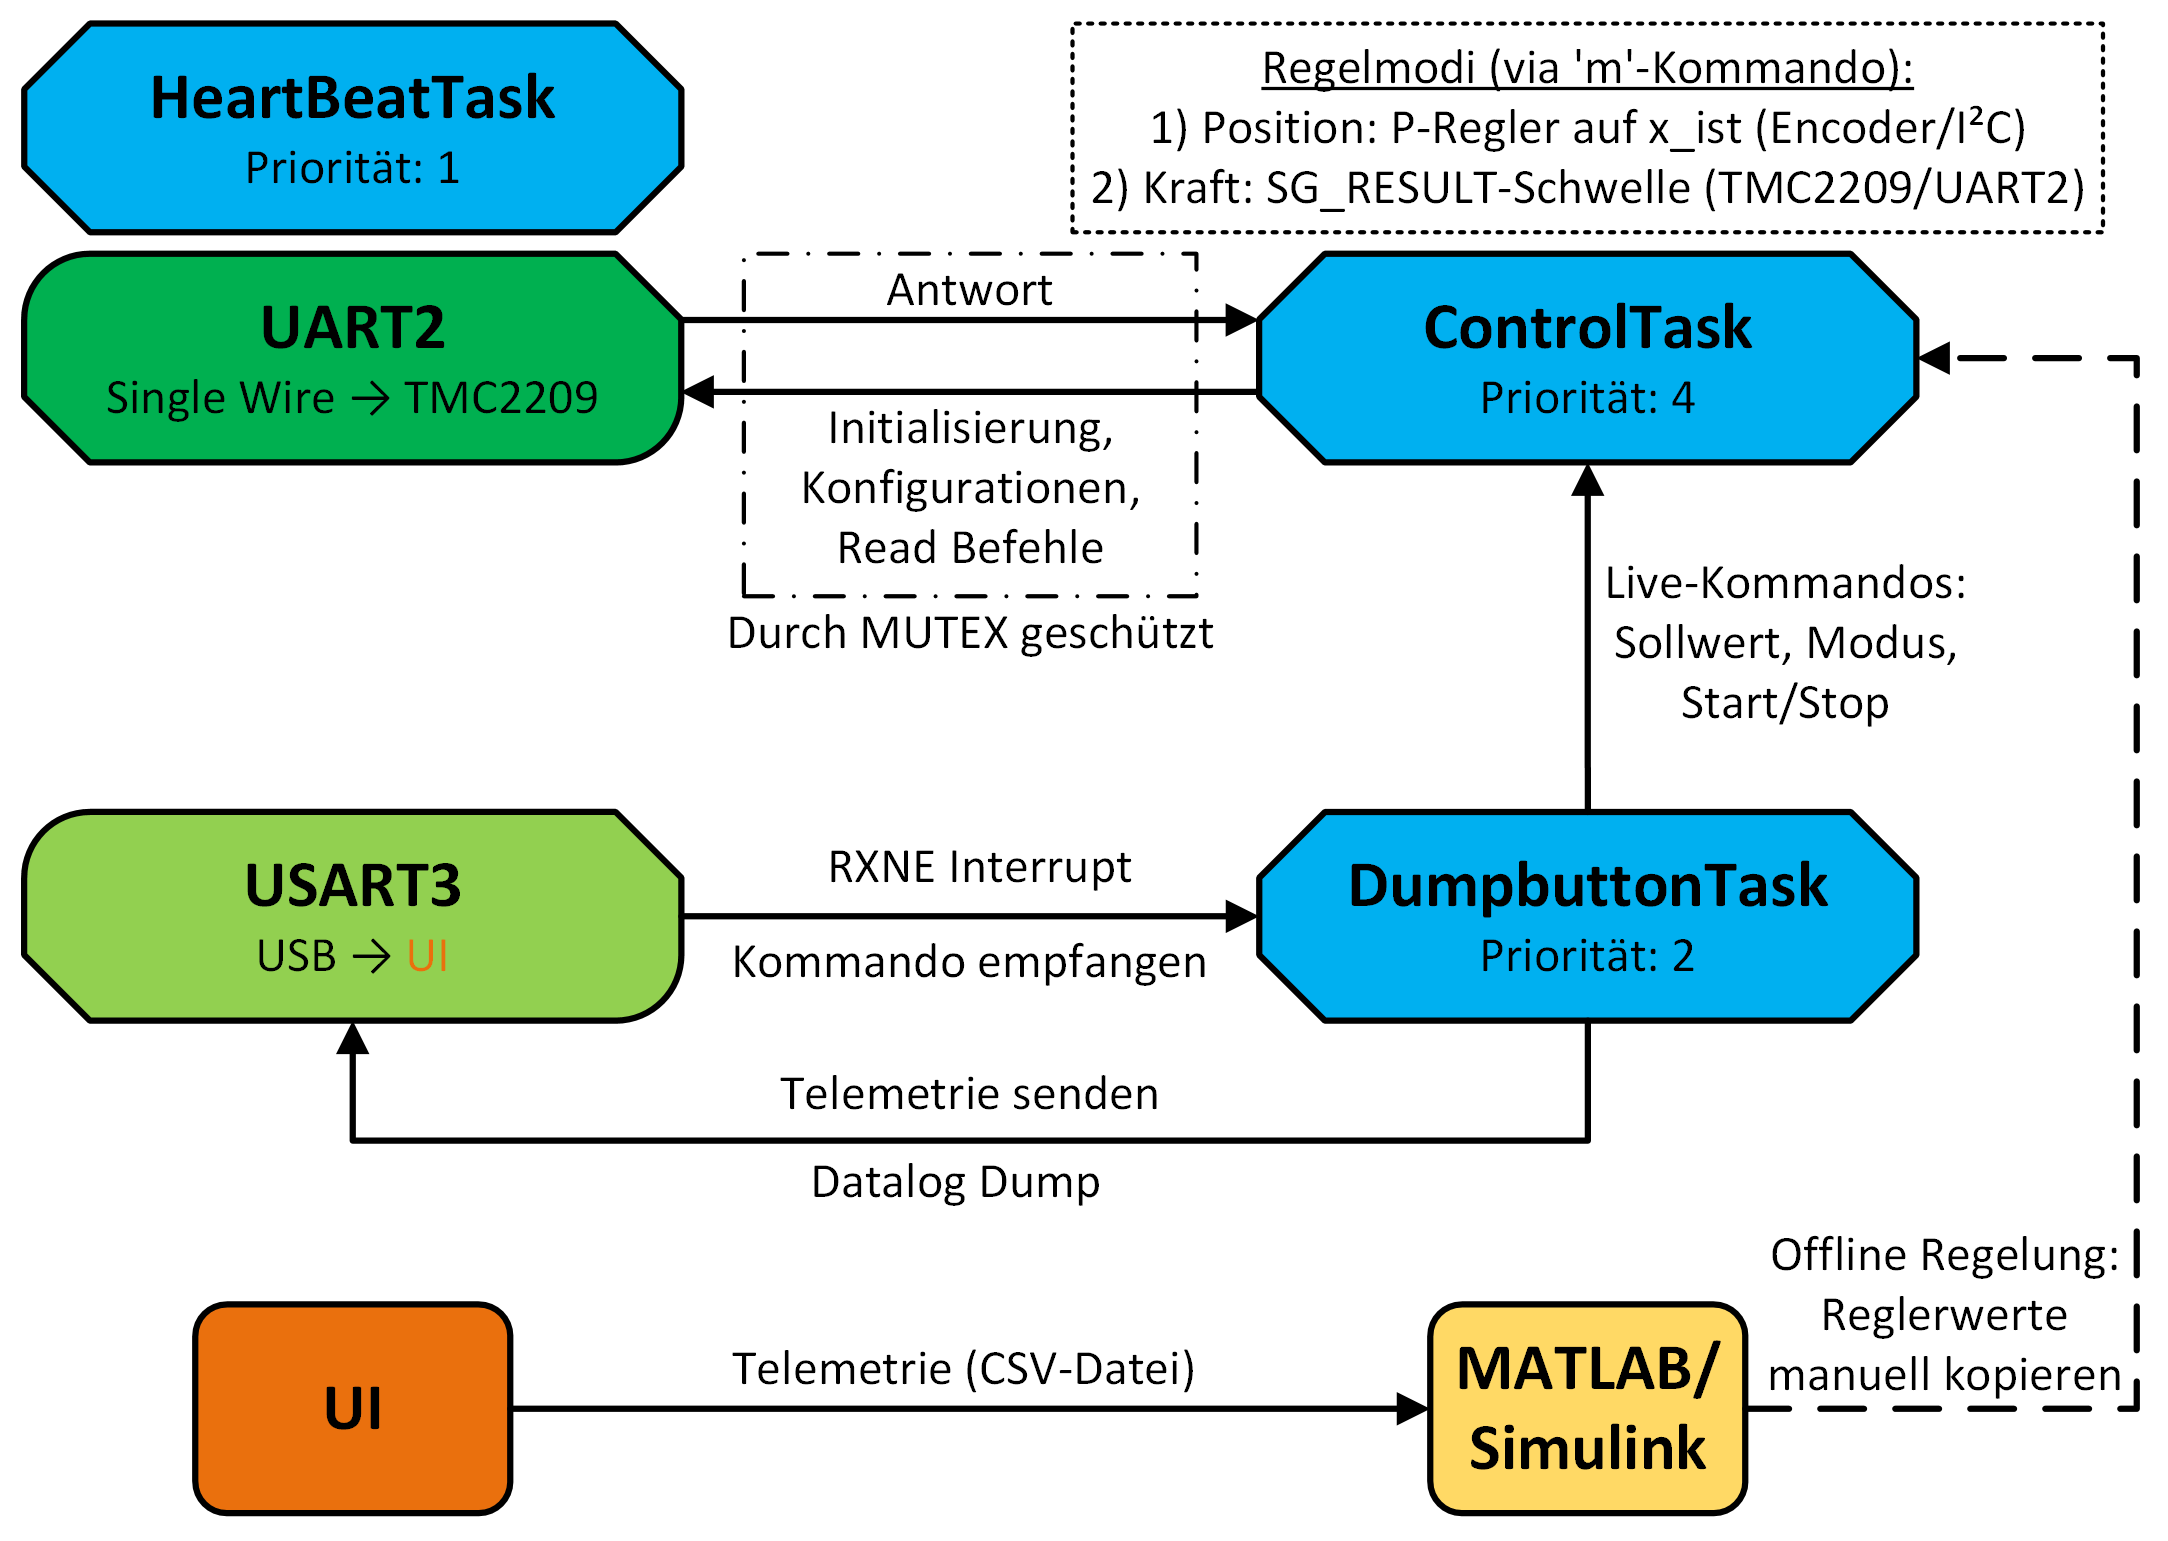
\includegraphics[width=0.85\linewidth]{Abbildung/Programmablauf.png}
    \caption{Grober Programmablauf}
    \label{fig:Programmablauf}
\end{figure}

Den höchstpriorisierten Task (Priorität~4) bildet der \textit{ControlTask}, der in einem festen 2\,ms-Zyklus die eigentliche Regelung ausführt. Er durchläuft einen Zustandsautomaten (\texttt{ST\_ZERO} $\rightarrow$ \texttt{ST\_DIRDETECT} $\rightarrow$ \texttt{ST\_CONTROL} $\rightarrow$ \texttt{ST\_HOLD}/\texttt{ST\_OPEN}/\texttt{ST\_FAULT}) und kann innerhalb des Regelzustands zwischen zwei Reglermodi umschalten, die über ein per USART3 empfangenes \texttt{m}-Kommando ausgewählt werden:

\begin{itemize}
    \item \textbf{Positionsregelung}: Ein P-Regler mit Totzone, Sättigung und Rate-Limiter regelt die Ist-Position (aus dem AS5600-Encoder, I\textsuperscript{2}C) auf einen vorgegebenen Sollwert.
    \item \textbf{Kraft-/Drehmomentregelung}: Auswertung des StallGuard-Werts (\texttt{SG\_RESULT}) des TMC2209-Treibers. Bei Unterschreiten eines vorgegebenen SG-Schwellwerts wird der Vorschub angehalten (indirekte Kraftregelung).
\end{itemize}

Die Kommunikation mit dem Motortreiber erfolgt über \textbf{UART2} als Single-Wire-Verbindung (Halbduplex). Über diese Schnittstelle werden sowohl die einmalige Initialisierung und Konfiguration (Mikroschrittauflösung, Motorstrom) als auch zyklische Lesebefehle (\texttt{SG\_RESULT} für die Kraftregelung) sowie die Geschwindigkeitsvorgaben (\texttt{VACTUAL}) abgewickelt. Da UART2 im Halbduplexbetrieb sowohl vom \texttt{ControlTask} als auch potenziell von parallelen Zugriffen genutzt werden könnte, ist jede Transaktion durch einen Mutex abgesichert.

Der zweite Task, \textit{DumpButtonTask} (Priorität~2), übernimmt die Kommunikation mit der Bedienoberfläche (UI) über \textbf{USART3} (USB-Verbindung). Eingehende Bytes werden zunächst per RXNE-Interrupt in einen Ringpuffer geschrieben. Der Task selbst pollt diesen Puffer alle 20\,ms, parst empfangene Kommandozeilen und setzt daraus globale Zustandsvariablen für Sollwert, Reglermodus und Start-/Stopp-/Öffnen-Befehle. Diese Variablen werden vom \textit{ControlTask} in jedem Regelzyklus ausgelesen und bilden damit den zentralen Steuerkanal zwischen UI und Regelung. Umgekehrt sendet der \textit{DumpButtonTask} periodisch einen Telemetrie-Datensatz sowie einen vollständigen CSV-Dump des Ringpuffer-Datenloggers über dieselbe Schnittstelle an die UI.

Der dritte Task, \textit{}{HeartBeatTask} (Priorität~1), blinkt eine LED im 1\,Hz-Takt und dient lediglich dem Nachweis, dass der Scheduler läuft.

Die von der UI empfangenen Telemetriedaten (CSV-Datei) werden außerhalb der Firmware in MATLAB/Simulink zur Reglerauslegung und -analyse weiterverarbeitet. Die ermittelten Parameter werden manuell als Konstanten in den Quellcode des \textit{ControlTask} übernommen.




% +++++++++++++++++++++++++++++++++++++++++++++++++++++++++++++++++
% Konfiguration von FreeRTOS
% +++++++++++++++++++++++++++++++++++++++++++++++++++++++++++++++++
\section{Konfiguration der MCU und von FreeRTOS}
Die Konfiguration des NUCLEO-F767ZI-Boards wurde in der Entwicklungsumgebung STM32CubeIDE mit dem Firmware Package \textit{STM32Cube FW\_F7 V1.17.3} wie folgt vorgenommen. Nicht explizit genannte Konfigurationen entsprechen den Standardeinstellungen der STM32CubeIDE:

\begin{itemize}
    \item Input Frequenz bei 8 MHz über die HSE und HCLK bei 216 MHz.
    
    \item Timer
    \begin{itemize}
        \item TIM8 als Timebase Source.
        \item TIM3 für Motorbewegungen mit einem Prescaler von 107, sodass unter Betrachtung der APB1 Clock (108 MHz) ein Zähltakt von 1 MHz vorliegt (eine Mikrosekunde pro Tick). TIM3 global interrupt aktiviert.
        \item TIM2 als freilaufender, vom Debugger unabhängiger 32-Bit-Zähler (ein Zählerstand entspricht einer Mikrosekunde) dient als Zeitbasis bzw. liefert Zeitstempel für das Loggen einer Regelabtastung.
    \end{itemize}
    \item USART
    \begin{itemize}
        \item USART2 mit einer Baudrate von 115200 und in der Mode Single Wire (Half Duplex). Pin PD5 wird ohne Pull initialiert.
        \item USART3 mit einer Baudrate von 500000, in Tx\_Rx-Mode und USART3\_IRQn aktiviert. Die Pins PD8 und PD9 werden ohne Pull initialisiert.
    \end{itemize}
    \item GPIO
    \begin{itemize}
        \item Pin PB0 als Output mit User Label \textit{LED\_GREEN}.
        \item Pin PE9 als Output mit Maximum Output Speed auf High und User Label \textit{TMC\_STEP}.
        \item Pin PE11 als Output mit User Label \textit{TMC\_DIR}.
        \item Pin PE13 als Output mit User Label \textit{TMC\_EN}.
    \end{itemize}
    \item GPIO I2C
    \begin{itemize}
        \item Pin PB8 als I2C1\_SCL Signal ohne Pull.
        \item Pin PB9 als I2C1\_SDA Signal ohne Pull.
    \end{itemize}
    \item GPIO NVIC: EXTI line[15:10] interrupts aktiviert.
    \item FreeRTOS Interface Version \textit{CMSIS\_V1}
    \begin{itemize}
        \item USE\_IDLE\_HOOK aktiviert.
        \item USE\_NEWLIB\_REENTRANT aktiviert.
    \end{itemize}
    
\end{itemize}


% +++++++++++++++++++++++++++++++++++++++++++++++++++++++++++++++++
% Motorsteuerung
% +++++++++++++++++++++++++++++++++++++++++++++++++++++++++++++++++
\section{Motorsteuerung}

Die Ansteuerung des Schrittmotors gliedert sich in zwei Softwareebenen: einen registerorientierten UART-Treiber für den Motortreiber TMC2209 (\texttt{tmc2209.h}/\texttt{tmc2209.c}) und eine darüberliegende Motor-Control-Schicht (\texttt{motor\_control.h}/\texttt{motor\_control.c}), die diesen Treiber initialisiert und zusätzliche Bewegungsoptionen bereitstellt.

\subsection{TMC2209-UART-Treiber}

Der TMC2209 wird ausschließlich über die Single-Wire-UART-Schnittstelle  parametriert und angesteuert. Die STEP/DIR-Pins des Treibers selbst kommen nicht zum Einsatz. Das Datagrammformat folgt dem Treiber-Datenblatt: Schreibzugriffe bestehen aus Sync-Byte, Slave-Adresse, Registeradresse (Bit~7 gesetzt) sowie 4 Datenbytes und einem CRC8-Prüfbyte. Lesezugriffe senden eine 4-Byte-Anfrage und erhalten eine 8-Byte-Antwort mit demselben Rahmenaufbau. Die CRC-Berechnung ist in der Funktion \texttt{tmc\_crc()} implementiert und wird sowohl beim Senden als auch beim Validieren empfangener Rahmen verwendet.

Da die Verbindung halbduplex betrieben wird, muss der UART-Treiber vor jedem Lesevorgang explizit vom Sende- in den Empfangsmodus umgeschaltet werden (\texttt{HAL\_HalfDuplex\_ EnableTransmitter}/\texttt{-EnableReceiver}). Gekapselt wird dieser Ablauf durch \texttt{TMC2209\_ Write()} und \texttt{TMC2209\_Read()}: Die beiden Funktionen sichern die gesamte Transaktion – Senden und Empfangen – über einen gemeinsamen Mutex (\texttt{drv->mutex}) ab, sodass parallele Zugriffe verschiedener Tasks auf denselben Bus nicht ineinandergreifen können. Ein Lesevorgang, der den Mutex nicht binnen 50\,ms erhält, wird mit \texttt{false} quittiert anstatt zu blockieren.

Auf dieser Transportschicht setzen mehrere Konfigurations- und Steuerfunktionen auf:
\begin{itemize}
    \item \texttt{TMC2209\_Init()} aktiviert per \texttt{GCONF}-Register die UART-Steuerung (\texttt{pdn\_disable}, \texttt{mstep\_reg\_select}), löscht latente Fehlerflags (\texttt{GSTAT}), aktiviert den Chopper (\texttt{CHOPCONF}, \texttt{TOFF=3}) und liest \texttt{GCONF} zur Verifikation zurück. Schlägt der Chip nicht an, meldet die Funktion \texttt{false}.
    \item \texttt{TMC2209\_SetCurrent()} setzt Lauf- und Haltestrom über das \texttt{IHOLD\_IRUN}-Register (je 0–31, entspricht 1/32 bis 32/32 des Skalenendwerts).
    \item \texttt{TMC2209\_SetMicrosteps()} setzt die Mikroschrittauflösung über das \texttt{MRES}-Feld in \texttt{CHOPCONF} (256 bis 1 Mikroschritte je Vollschritt).
    \item \texttt{TMC2209\_SetStallguardThreshold()} und \texttt{TMC2209\_SeCoolStepThreshold ()} konfigurieren StallGuard4 (\texttt{SGTHRS}) bzw. dessen Gültigkeitsfenster (\texttt{TCOOLTHRS}). Beide Werte bilden die Grundlage für die im \texttt{ControlTask} realisierte StallGuard-basierte Kraftregelung.
    \item \texttt{TMC2209\_MoveVelocity()} schreibt eine Solldrehzahl in das \texttt{VACTUAL}-Register (24 Bit, mit Vorzeichen). In diesem Betriebsmodus erzeugt der TMC2209 die Mikroschritt-Pulse intern. Der Microcontroller muss keine STEP-Flanken mehr ausgeben. \texttt{TMC2209\_Stop()} setzt \texttt{VACTUAL} auf 0.
\end{itemize}

\subsection{Motor-Control-Schicht}

Die Datei \texttt{motor\_control.c} bündelt die Inbetriebnahme des Treibers und stellt zwei alternative Mechanismen zur Bewegungserzeugung bereit, die im Code parallel existieren, aber unterschiedlich stark genutzt werden.

Die Funktion \texttt{MotorControl\_Init()} ruft \texttt{TMC2209\_Init()} in einer Retry-Schleife auf (Wiederholung alle 500\,ms bis zur erfolgreichen Antwort), setzt anschließend feste Betriebsparameter (16 Mikroschritte, \texttt{IRUN=IHOLD=27} für ca.\ 0{,}86\,A\textsubscript{RMS} bei $R_\text{sense}=0{,}11\,\Omega$, ein konservatives StallGuard/CoolStep-Fenster) und aktiviert den Treiber über den Enable-Pin. Über \texttt{MotorControl\_GetDriver()} erhalten andere Module (insbesondere der \texttt{ControlTask}) Zugriff auf den initialisierten TMC2209-Handle, um darüber \texttt{TMC2209\_MoveVelocity()} bzw.\ \texttt{TMC2209\_Read()} (StallGuard) direkt aufzurufen. Durch diesen UART/VACTUAL-Pfad kann der geschlossene Regelkreis im \textit{ControlTask} über \texttt{TMC2209\_MoveVelocity()} kommandiert werden.


% +++++++++++++++++++++++++++++++++++++++++++++++++++++++++++++++++
% Taskeinbindung der Regler
% +++++++++++++++++++++++++++++++++++++++++++++++++++++++++++++++++
\section{Einbindung der Regler in die Taskstruktur}
\label{sec:taskeinbindung}
\textit{Bearbeitet von Mohammad Badr Eddin}\\
Die Firmware basiert auf FreeRTOS. Beide in Kapitel \ref{Kap:Regler}
beschriebenen Regler laufen gemeinsam im zyklischen
\texttt{ControlTask}. Sie verwenden dieselbe Messgröße des AS5600 über
I\textsuperscript{2}C und dieselbe Stellgröße über \texttt{VACTUAL}.
Da immer nur ein Regler aktiv ist, ist eine Aufteilung auf getrennte
Tasks nicht erforderlich.

Der \texttt{ControlTask} besitzt die höchste Priorität aller Tasks.
Sein Regelzyklus wird über eine absolute Zeitbasis auf
\SI{2}{\milli\second} festgelegt. Dadurch bleibt der zeitliche Abstand
zwischen den einzelnen Zyklen unabhängig von der Laufzeit des
Taskrumpfs konstant. Der Zeitstempel für die Messdaten wird direkt
nach dem Aufwecken des Tasks erfasst.

Innerhalb eines Zyklus werden die folgenden Schritte durchlaufen:

\begin{enumerate}
    \item Zeitstempel erfassen,
    \item Encoderwert über I\textsuperscript{2}C lesen und zur
          Istposition verarbeiten,
    \item Treiberstatus über die UART auslesen,
    \item Bedienkommandos und Sollwerte übernehmen,
    \item Zustandsautomat und aktiven Regler ausführen,
    \item Stellgröße als Sollgeschwindigkeit an den Treiber senden,
    \item Messwerte im Ringpuffer speichern.
\end{enumerate}

Die Auswahl des Positions- oder Effort-Reglers richtet sich nach der
aktuellen Betriebsart. Pro Zyklus berechnet nur einer der beiden
Regler die Stellgröße. Die gemeinsame Encoderauswertung,
Stellgrößenbegrenzung und Messdatenspeicherung werden unabhängig von
der Betriebsart nur einmal ausgeführt.

Der Regelzyklus selbst enthält keine Datenausgabe. Die Messwerte
werden zunächst in einem Ringpuffer im Arbeitsspeicher gespeichert
und anschließend von einem niederpriorisierten Task über USART3
übertragen. Sollwerte und Bedienkommandos werden ebenfalls außerhalb
des Regelzyklus in gemeinsamen Variablen hinterlegt. Der
\texttt{ControlTask} übernimmt diese Werte an einer festgelegten
Stelle innerhalb seines Zyklus, sodass die laufende Berechnung nicht
unterbrochen wird.

Die Initialisierung des Motortreibers erfolgt am Anfang des
\texttt{ControlTask}, da sie blockierende UART-Transaktionen enthält.
Während dieser Phase bleibt die Endstufe über das Enable-Signal
abgeschaltet. Die UART-Zugriffe auf den Treiber werden über einen
Mutex geschützt, sodass gleichzeitige Transaktionen nicht
miteinander kollidieren.
% +++++++++++++++++++++++++++++++++++++++++++++++++++++++++++++++++
% Schutz
% +++++++++++++++++++++++++++++++++++++++++++++++++++++++++++++++++
\section{Überlast- und Kollisionsschutz}
\textit{Bearbeitet von Mohammad Badr Eddin}\\

Der Schrittmotor wird im Betrieb über vorgegebene Schrittimpulse
angesteuert. Kommt es zu einer mechanischen Blockade oder einer
Kollision der Greiferbacken, können weiterhin Schrittimpulse erzeugt
werden, obwohl sich der Antrieb nicht mehr bewegt. Eine solche
Situation wird über das Positionsfeedback des AS5600 erkannt. Die
gemessene Bewegung wird mit der vorgegebenen Bewegung des Antriebs
verglichen. Die bestehende Task- und Zustandsautomatenstruktur mit
einer Zykluszeit von \SI{2}{\milli\second} bleibt unverändert.

Für die Erkennung einer Blockade wird nicht nur die aktuelle
Positionsabweichung betrachtet. Während einer normalen Bewegung kann
diese ebenfalls auftreten und würde sonst zu einer fehlerhaften
Abschaltung führen.

Stattdessen wird der Positionsfortschritt über ein Zeitfenster von
\SI{0.15}{\second}, entsprechend 75 Regelzyklen, ausgewertet. Eine
Prüfung erfolgt nur, wenn während mindestens 80\,\% des Zeitfensters
eine ausreichende Bewegungsanforderung vorliegt. Die dafür festgelegte
Mindestgeschwindigkeit beträgt \SI{3}{\milli\meter\per\second}.

Bleibt der gemessene Positionsfortschritt innerhalb eines Zeitfensters
unter \SI{0.2}{\milli\meter}, wird dieses als fehlerhaft bewertet.
Erst drei aufeinanderfolgende fehlerhafte Fenster führen zur
Erkennung einer Blockade bzw. eines möglichen
Schrittverlusts. Die Überwachungsdauer beträgt somit insgesamt
\SI{0.45}{\second}.

Die zeitliche Auswertung verhindert, dass kurze Abweichungen während
der Beschleunigungs- und Bremsphasen oder bei einer Änderung des
Sollwerts unmittelbar eine Abschaltung auslösen.

Wird eine Blockade erkannt, beendet die Steuerung den regulären
Regelbetrieb und wechselt in den Zustand \texttt{ST\_FAULT}. Der Motor
wird über die vorhandene Stopp-Funktion des Treibers angehalten. Im
Fehlerzustand ist die Motoransteuerung durch die Positions- und
Effort-Regelung gesperrt, sodass der Antrieb nicht selbstständig wieder
starten kann. Eine erneute Inbetriebnahme erfolgt erst nach einem
bewussten Neustart der Steuerung. Nach dem Neustart werden die
Initialisierung und die Richtungserkennung erneut durchgeführt.

% % +++++++++++++++++++++++++++++++++++++++++++++++++++++++++++++++++
% % Benutzeroberfläche
% % +++++++++++++++++++++++++++++++++++++++++++++++++++++++++++++++++
% \section{Benutzeroberfläche}
% \textit{Bearbeitet von Masoud Fahim}\\

% [\textit{Umsetzung der UI u.a. zum Umschalten des Reglers}]



\bigskip

% ---------------------------------------------------------
% Testlauf & Resultate
% ---------------------------------------------------------
\chapter{Testlauf und Resultate}\label{Kap:Testlauf}
% =================================================================
% Kapitel: Testlauf und Ergebnisse
% =================================================================

% +++++++++++++++++++++++++++++++++++++++++++++++++++++++++++++++++
% Echtzeitfähigkeit
% +++++++++++++++++++++++++++++++++++++++++++++++++++++++++++++++++
\section{Echtzeitfähigkeit}
\label{sec:ergebnis_echtzeit}

Die Anforderung an die Echtzeitfähigkeit verlangt eine definierte, deterministische
Zykluszeit. Der im Aufgabenblatt genannte Wert von 1~ms ist dabei als Beispiel angegeben;
gefordert ist der Determinismus, nicht ein bestimmter Zahlenwert.

\subsection*{Wahl der Zykluszeit}

Der Reglertask läuft mit einer Periode von 2~ms. Diese Wahl folgt aus der in Abschnitt
\ref{sec:positionsregler} festgelegten Bandbreite von 20~Hz. Mit einer Abtastfrequenz von
500~Hz liegt zwischen Bandbreite und Abtastrate ein Faktor von 25, womit die
Diskretisierung das Verhalten des Kreises nicht dominiert. Der in Gleichung
\ref{eq:polstelle} berechnete Wert $K_P T = 0{,}251$ bestätigt dies: Der Kreis baut pro
Takt nur ein Viertel der verbleibenden Abweichung ab und bleibt damit weit von der
Stabilitätsgrenze der Abtastung entfernt.

Eine Halbierung auf 1~ms würde die Regelgüte nicht verbessern, da die Bandbreite durch die
Motordynamik und nicht durch die Abtastung begrenzt ist. Sie würde das Zeitbudget des
Tasks jedoch halbieren und damit die im Folgenden beschriebene Problematik verschärfen.

\subsection*{Messung}

Zur Beurteilung der Zykluszeit wurde in der Firmware ein Zeitstempel aus einem
Hardware-Timer erfasst und im Ringpuffer mitgeschrieben. Der Zeitstempel wird unmittelbar
nach der Rückkehr aus \texttt{vTaskDelayUntil} genommen, also vor sämtlichen Lese-, Rechen-
und Schreibvorgängen des Zyklus. Er misst damit den tatsächlichen Weckzeitpunkt des Tasks
und nicht die Laufzeit innerhalb des Zyklus. Die Auswertung erfolgte über das Skript
\texttt{gripper\_log.m} anhand der Aufzeichnung \texttt{jitter\_test.csv}.

% ---------------------------------------------------------------
\begin{table}[htbp]
    \centering
    \caption{Gemessene Zykluszeit des Reglertasks}
    \label{tab:jitter}
    \begin{tabular}{ll}
        \hline
        Größe & Wert \\
        \hline
        Sollperiode                 & 2000~$\mu$s \\
        gemessene mittlere Periode  & 2000~$\mu$s \\
        Standardabweichung          & 349~$\mu$s \\
        Wertebereich                & 1447 \ldots 2553~$\mu$s \\
        \hline
    \end{tabular}
\end{table}
% ---------------------------------------------------------------

\subsection*{Der Jitter ist deterministisch, nicht zufällig}

Die Standardabweichung von 349~$\mu$s entspricht 17~\% der Sollperiode und wirkt zunächst
erheblich. Sie ist an dieser Stelle jedoch die irreführende Kennzahl. Eine
Standardabweichung beschreibt die Streuung um einen Mittelwert und legt damit zufälliges
Rauschen nahe. Die gemessene Verteilung ist dagegen nicht kontinuierlich, sondern
\emph{trimodal}: Die Perioden nehmen im Wesentlichen nur drei Werte an, wie Abbildung
\ref{fig:jitter_histogramm} zeigt.

% ---------------------------------------------------------------
\begin{figure}[htbp]
    \centering
    % \includegraphics[width=0.8\textwidth]{bilder/jitter_histogramm.pdf}
    \caption{Verteilung der gemessenen Zykluszeit. Drei von fünf Zyklen treffen die
             Sollperiode exakt; die beiden Nebenmaxima liegen symmetrisch um
             $\pm 550$~$\mu$s.}
    \label{fig:jitter_histogramm}
\end{figure}
% ---------------------------------------------------------------

% ---------------------------------------------------------------
\begin{table}[htbp]
    \centering
    \caption{Verteilung der gemessenen Periodendauer}
    \label{tab:jitter_verteilung}
    \begin{tabular}{lll}
        \hline
        Periodendauer & Anteil & Abweichung vom Sollwert \\
        \hline
        2000~$\mu$s & 60~\% & 0 \\
        1450~$\mu$s & 20~\% & $-550$~$\mu$s \\
        2550~$\mu$s & 20~\% & $+550$~$\mu$s \\
        \hline
    \end{tabular}
\end{table}
% ---------------------------------------------------------------

Die Ursache dieser Struktur ist bekannt und reproduzierbar. Jeder fünfte Zyklus liest
\texttt{SG\_RESULT} über die UART-Verbindung zum Treiber. Dieser Zugriff ist blockierend
und dauert bei der eingestellten Baudrate rund 1,4~ms. Zusammen mit dem übrigen
Zyklusinhalt überschreitet dieser Zyklus die Periodendauer, sodass der Folgezyklus
verspätet geweckt wird. Anschließend fängt sich der Takt wieder ein, was die symmetrische
Abweichung von $\pm 550~\mu$s erklärt.

Die zutreffende Beschreibung lautet daher: Der Takt ist nicht verrauscht, sondern
periodisch gestört, mit bekannter Ursache und bekannter Periodizität.

\subsection*{Bewertung gegen die Anforderung}

Die Anforderung zerfällt in drei Teilaussagen, die getrennt zu beurteilen sind.

% ---------------------------------------------------------------
\begin{table}[htbp]
    \centering
    \caption{Bewertung der Echtzeitanforderung}
    \label{tab:echtzeit_bewertung}
    \begin{tabular}{lp{8cm}}
        \hline
        Teilaussage & Ergebnis \\
        \hline
        kein Drift
            & erfüllt. Die mittlere Periode trifft den Sollwert exakt; die Bindung an den
              Systemtakt über \texttt{vTaskDelayUntil} schließt einen kumulierenden Fehler
              strukturell aus \\[0.4em]
        Ursache bekannt und reproduzierbar
            & erfüllt. Die Störung tritt in jedem fünften Zyklus auf und ist auf einen
              einzelnen Registerzugriff zurückführbar \\[0.4em]
        jeder einzelne Zyklus hält die Frist ein
            & nicht erfüllt. In jedem fünften Zyklus wird die Periodendauer überschritten \\
        \hline
    \end{tabular}
\end{table}
% ---------------------------------------------------------------

Der dritte Punkt ist offen zu benennen. Dass der Mittelwert den Sollwert trifft, bedeutet
lediglich, dass sich der Takt nach einer Überschreitung wieder einfängt, nicht dass die
Frist eingehalten wurde. Im Sinne einer harten Echtzeitbedingung ist die Anforderung damit
nicht vollständig erfüllt.

\subsection*{Auswirkung auf die Regelgüte}

Trotz dieser Einschränkung ist keine Auswirkung auf die Regelgüte messbar, und das ist
kein Zufall, sondern eine Folge der gewählten Reglerstruktur.

In der Rechenvorschrift des Positionsreglers, $v = K_P \cdot e$, kommt die Abtastzeit
nicht vor. Es wird weder über $T$ integriert noch nach $T$ differenziert. Eine
schwankende Periodendauer verschiebt daher ausschließlich den Zeitpunkt, zu dem eine
Stellgröße ausgegeben wird, nicht aber deren Wert. Ein PI-Regler wäre an dieser Stelle
empfindlich gewesen: Sein Integralanteil hätte bei einer um 27~\% zu langen oder zu
kurzen Periode einen entsprechenden Fehler aufsummiert.

Die einzige Ausnahme bildet die Anstiegsbegrenzung, die den je Takt zulässigen
Geschwindigkeitssprung als $\Delta v = a_{max} \cdot T$ berechnet. Eine Abweichung von
550~$\mu$s entspricht hier einem Fehler von rund 27~\% im zulässigen Sprung. Da die
Anstiegsbegrenzung ausschließlich beim Anfahren großer Sollwertsprünge wirksam wird und
die in Abschnitt \ref{sec:ergebnis_position} nachgewiesene Positioniergenauigkeit
unterhalb von 0,05~mm liegt, bleibt dieser Effekt ohne messbare Folge.

\subsection*{Möglichkeit zur Beseitigung}

Da \texttt{SG\_RESULT} für die umgesetzte Kraftvorgabe nicht mehr benötigt wird, ließe
sich die Ursache des Jitters vollständig beseitigen, indem der Registerzugriff aus dem
Reglertakt entfernt wird. Die Periodendauer läge dann auf der Auflösung des Systemtakts.
Darauf wurde bewusst verzichtet, um die vorliegenden Messreihen nicht auf einem anderen
Firmwarestand zu erheben als die hier dokumentierte Zeitmessung. Eine alternative
Entschärfung wäre die Erhöhung der Baudrate zum Treiber, die den Zugriff auf unter ein
Drittel der bisherigen Dauer verkürzen würde.

% +++++++++++++++++++++++++++++++++++++++++++++++++++++++++++++++++
% Positioniergenauigkeit
% +++++++++++++++++++++++++++++++++++++++++++++++++++++++++++++++++
\section{Positioniergenauigkeit}
\label{sec:ergebnis_position}

Die Anforderung verlangt, die Fingerposition mit einer Genauigkeit von $\pm 0{,}5$~mm
anfahren zu können.

\subsection*{Versuchsdurchführung}

Zur Überprüfung wurde eine Folge von Zielpositionen von 10, 20, 30, 40 und 50~mm
angefahren und die vom Encoder gemessene Position aufgezeichnet
(\texttt{Test03pos.csv}). Die gestufte Vorgabe prüft die Genauigkeit nicht an einem
einzelnen Punkt, sondern über den gesamten genutzten Verfahrbereich, sodass ein
systematischer Fehler in der Umrechnung von Encoderzählschritten in Millimeter als
wachsende Abweichung sichtbar würde.

% ---------------------------------------------------------------
\begin{figure}[htbp]
    \centering
    % 
\includegraphics[width=\textwidth]{bilder/positionstreppe.pdf}
    \caption{Sollwertfolge und gemessene Position über den Verfahrbereich. Die
             Zustellbewegungen erfolgen über den überwiegenden Teil der Strecke mit
             Höchstgeschwindigkeit.}
    \label{fig:positionstreppe}
\end{figure}
% ---------------------------------------------------------------

\subsection*{Ergebnis}

Die bleibende Abweichung liegt bei allen angefahrenen Positionen unterhalb von 0,05~mm.
Gegenüber der geforderten Genauigkeit von $\pm 0{,}5$~mm besteht damit ein
Sicherheitsfaktor von zehn. Die Anforderung ist erfüllt.

% ---------------------------------------------------------------
\begin{table}[htbp]
    \centering
    \caption{Bleibende Abweichung der angefahrenen Positionen}
    \label{tab:positioniergenauigkeit}
    \begin{tabular}{lll}
        \hline
        Zielposition & gemessene Position & Abweichung \\
        \hline
        10~mm & \textit{[Wert aus Test03pos.csv]} & \textit{[Wert]} \\
        20~mm & \textit{[Wert aus Test03pos.csv]} & \textit{[Wert]} \\
        30~mm & \textit{[Wert aus Test03pos.csv]} & \textit{[Wert]} \\
        40~mm & \textit{[Wert aus Test03pos.csv]} & \textit{[Wert]} \\
        50~mm & \textit{[Wert aus Test03pos.csv]} & \textit{[Wert]} \\
        \hline
    \end{tabular}
\end{table}
% ---------------------------------------------------------------

\subsection*{Einordnung des Ergebnisses}

Der gemessene Wert ist kein zufälliges Resultat, sondern entspricht der Erwartung aus der
Auslegung. Die Totzone des Reglers beträgt nach Abschnitt \ref{sec:positionsregler}
0,05~mm. Innerhalb dieses Bereichs wird die Regelabweichung bewusst nicht mehr korrigiert,
um den in Abschnitt \ref{sec:sim_position} beschriebenen Grenzzyklus zu vermeiden. Die
bleibende Abweichung muss folglich in genau dieser Größenordnung liegen.

Damit ist zugleich die systembedingte Untergrenze erreicht. Eine weitere Verbesserung
ließe sich nicht durch eine höhere Reglerverstärkung oder eine kürzere Zykluszeit
erzielen, sondern ausschließlich durch eine Verkleinerung der Totzone -- und die ist durch
das Verhältnis von Mikroschritt zu Encoderauflösung nach unten begrenzt. Solange der
kleinste Stellschritt des Aktors größer ist als die kleinste auflösbare Messgröße, führt
jede feinere Einstellung zum Pendeln statt zu höherer Genauigkeit.

Die erreichte Genauigkeit ist somit keine Eigenschaft der Reglerparametrierung, sondern
eine Eigenschaft der gewählten Hardwarekombination aus Mikroschrittauflösung und
Encoder. Für eine höhere Genauigkeit wäre entweder eine feinere Mikroschrittteilung oder
ein höher auflösender Encoder erforderlich.

\subsection*{Anmerkung zum Zeitverhalten}

Die in Abbildung \ref{fig:positionstreppe} sichtbaren Zustellbewegungen sind nicht zur
Beurteilung der Reglerdynamik geeignet. Bei einer Schrittweite von 10~mm arbeitet der
Regler über 0,24~s in der Stellgrößenbegrenzung und erreicht erst auf den letzten
0,32~mm seinen linearen Bereich. Der sichtbare Verlauf ist damit im Wesentlichen eine
Fahrt mit konstanter Höchstgeschwindigkeit. Zur Verifikation der Reglerverstärkung sind
ausschließlich Sprünge unterhalb von 0,3~mm geeignet, wie in Abschnitt
\ref{sec:sim_position} hergeleitet.

% +++++++++++++++++++++++++++++++++++++++++++++++++++++++++++++++++
% Greifkraft und Umschaltbarkeit
% +++++++++++++++++++++++++++++++++++++++++++++++++++++++++++++++++
\section{Greifkraft und Umschaltbarkeit}
\label{sec:ergebnis_kraft}

Die Anforderung verlangt, dass die aufgebrachte Greifkraft in einem definierten Bereich
stufenlos vorgebbar ist und dass zwischen Positions- und Kraftbetrieb während des Betriebs
umgeschaltet werden kann.

\subsection*{Versuchsdurchführung}

Der Prüfstand bildet ein nachgiebiges Greifobjekt durch zwei parallel angeordnete Federn
nach, die von der Zahnstange zusammengedrückt werden. Die wirksame Steifigkeit beträgt
$c_{eff} = 2{,}12$~N/mm.

Je Versuch wurde der Finger zunächst positionsgeregelt zugestellt, bis die Federn gerade
berührt wurden. Diese Position wurde als Kontaktpunkt $x_0$ übernommen. Anschließend
erfolgte die Umschaltung in den Kraftbetrieb und die Vorgabe der Zielkraft. Die
tatsächlich aufgebrachte Kraft wurde nach Gleichung \ref{eq:kraft_rueckrechnung} aus der
gemessenen Position berechnet. Die Aufzeichnung erfolgte in
\texttt{Test05Effort\_Pose.csv}.

% ---------------------------------------------------------------
\begin{figure}[htbp]
    \centering
    % \includegraphics[width=\textwidth]{bilder/kraftverlauf_messung.pdf}
    \caption{Gemessener Kraftverlauf beim Anfahren der Zielkraft. Bis zum Kontaktpunkt
             bleibt die Kraft null, anschließend baut sie sich mit der Zustellbewegung auf
             und bleibt nach Erreichen der Zielposition konstant.}
    \label{fig:kraftverlauf_messung}
\end{figure}
% ---------------------------------------------------------------

\subsection*{Ergebnis}

Tabelle \ref{tab:kraftmessung} fasst die erreichten Kräfte zusammen.

% ---------------------------------------------------------------
\begin{table}[htbp]
    \centering
    \caption{Erreichte Greifkraft bei $c_{eff} = 2{,}12$~N/mm}
    \label{tab:kraftmessung}
    \begin{tabular}{llll}
        \hline
        Sollkraft & Messwerte & maximale Abweichung & entspricht Wegfehler \\
        \hline
        5~N  & 4,98 / 4,92 / 4,95~N & $-0{,}08$~N \quad (1,6~\%) & 0,038~mm \\
        10~N & 9,92 / 9,95~N        & $-0{,}08$~N \quad (0,8~\%) & 0,038~mm \\
        \hline
    \end{tabular}
\end{table}
% ---------------------------------------------------------------

Die Abweichungen liegen bei beiden Zielkräften unterhalb von 1,6~\%. Die Kraft ist damit
über den geprüften Bereich vorgebbar, und die Anforderung ist erfüllt.

\subsection*{Einordnung}

Drei Beobachtungen sind hervorzuheben.

Erstens ist die absolute Abweichung bei beiden Zielkräften mit 0,08~N identisch. Das ist
zu erwarten, da der Fehler nach Gleichung \ref{eq:kraftfehler} aus der Positionsgenauigkeit
folgt und nicht von der Höhe der Zielkraft abhängt. Der relative Fehler halbiert sich
folglich beim Übergang von 5~N auf 10~N.

Zweitens liegen alle gemessenen Kräfte \emph{unterhalb} der Vorgabe. Diese Abweichung ist
systematisch und nicht zufällig. Sie erklärt sich aus der Totzone: Der Regler stellt seine
Bewegung ein, sobald die Regelabweichung die Totzone unterschreitet. Da die Zielposition
beim Greifen stets von unten angefahren wird, bleibt der Finger tendenziell knapp vor der
Zielposition stehen, der Federweg fällt geringfügig zu klein aus und damit auch die Kraft.
Ein systematischer Offset in dieser Größenordnung ließe sich durch eine geringfügig
erhöhte Zielposition kompensieren.

Drittens entsprechen alle gemessenen Abweichungen einem Wegfehler von höchstens 0,038~mm
und liegen damit innerhalb der Totzone von 0,05~mm. Das Ergebnis ist also vollständig durch
die bereits in Abschnitt \ref{sec:ergebnis_position} nachgewiesene Positioniergenauigkeit
erklärt. Ein zusätzlicher Fehlerbeitrag aus dem Federmodell oder aus der Bestimmung des
Kontaktpunkts ist in den Messwerten nicht erkennbar.

Der letzte Punkt ist bemerkenswert, weil die Fehlerbetrachtung in Tabelle
\ref{tab:fehlerquellen} den Kontaktpunkt als kritische Größe ausweist. Dass sich kein
entsprechender Beitrag zeigt, bedeutet, dass $x_0$ in den durchgeführten Versuchen auf
wenige Hundertstel Millimeter reproduzierbar getroffen wurde.

% ---------------------------------------------------------------
% HINWEIS an das Team, vor Abgabe entfernen:
% Prüfen, ob x0 in den drei 5-N-Läufen jeweils NEU gesetzt wurde.
% Falls dieselbe Kontaktposition wiederverwendet wurde, belegen die Werte
% nur die Wiederholgenauigkeit des Positionsreglers, nicht die des
% Gesamtverfahrens. Dann den letzten Absatz streichen und stattdessen
% schreiben: "Die Reproduzierbarkeit der Kontaktpunktbestimmung wurde
% nicht gesondert untersucht."
% ---------------------------------------------------------------

\subsection*{Umschaltbarkeit}

Die Umschaltung zwischen Positions- und Kraftbetrieb erfolgte in allen Versuchen im
laufenden Betrieb und ohne erkennbaren Sprung der Stellgröße. Das ist eine unmittelbare
Folge der in Abschnitt \ref{sec:zustandsautomat} beschriebenen Struktur: Beide
Betriebsarten verwenden denselben Regler, und beim Umschalten ändert sich ausschließlich
die Herkunft des Positionssollwerts. Es existieren keine Reglerzustände, die beim Wechsel
zu übergeben wären, und kein zweiter Regler, dessen Ausgangsgröße im Umschaltmoment von
der des ersten abweichen könnte.

Die geforderte nahtlose Umschaltung ist damit erfüllt. Sie ist im vorliegenden Entwurf
allerdings weniger eine gelöste Aufgabe als eine Eigenschaft, die sich aus der Wahl der
Kraftvorgabe von selbst ergibt.

% +++++++++++++++++++++++++++++++++++++++++++++++++++++++++++++++++
% Abgleich Simulation und Messung
% +++++++++++++++++++++++++++++++++++++++++++++++++++++++++++++++++
\section{Abgleich von Simulation und Messung}
\label{sec:ergebnis_abgleich}

Die in Kapitel \ref{chap:simulation} erstellten Modelle sind erst dann als
Vergleichsgrundlage brauchbar, wenn sie das reale Verhalten treffen. Dieser Abschnitt
stellt Simulation und Messung gegenüber.

\subsection*{Positionsverlauf}

Verglichen wurde der simulierte mit dem gemessenen Positionsverlauf bei identischer
Sollwertvorgabe. Die Messdaten stammen aus dem Ringpuffer der Firmware und liegen damit im
2-ms-Raster des Reglertasks vor, sodass kein Auflösungsverlust gegenüber der Simulation
entsteht.

% ---------------------------------------------------------------
\begin{figure}[htbp]
    \centering
    % \includegraphics[width=\textwidth]{bilder/abgleich_position.pdf}
    \caption{Gemessener und simulierter Positionsverlauf bei gleicher Sollwertvorgabe.}
    \label{fig:abgleich_position}
\end{figure}
% ---------------------------------------------------------------

Als Maß für die Übereinstimmung dient der mittlere quadratische Fehler über den gesamten
Verlauf. Er liegt unterhalb von 0,3~mm. Das Modell bildet damit sowohl die
Sättigungsfahrt als auch das Einlaufen in die Zielposition zutreffend ab.

\subsection*{Einordnung des Fehlermaßes}

Der Wert von 0,3~mm scheint zunächst im Widerspruch zu der in Abschnitt
\ref{sec:ergebnis_position} nachgewiesenen Positioniergenauigkeit von unter 0,05~mm zu
stehen. Beide Größen beschreiben jedoch Unterschiedliches.

Die Positioniergenauigkeit bezieht sich auf den stationären Endwert. Der mittlere
quadratische Fehler wird dagegen über den gesamten Verlauf einschließlich der
Zustellbewegung gebildet. Während dieser Bewegung fährt der Antrieb mit 40~mm/s, sodass
bereits ein geringfügiger zeitlicher Versatz zwischen Modell und Messung einen
erheblichen Beitrag zum Fehlermaß liefert: Ein Versatz von 7,5~ms entspricht bei dieser
Geschwindigkeit genau 0,3~mm.

Der ausgewiesene Wert ist damit im Wesentlichen ein Maß für die zeitliche Synchronisation
zwischen Simulation und Messung und nicht für eine Abweichung im Verhalten. Ursachen für
einen solchen Versatz sind der genaue Zeitpunkt, zu dem das Sollwertkommando in der
Firmware wirksam wird, sowie die Toleranz des internen Taktgenerators des Treibers, der
die Schrittfrequenz und damit die tatsächliche Verfahrgeschwindigkeit bestimmt.

\subsection*{Kraftverlauf}

Für den Kraftzweig wurde der in Abschnitt \ref{sec:sim_feder} simulierte Greifvorgang dem
gemessenen Verlauf aus \texttt{Test05Effort\_Pose.csv} gegenübergestellt. Da die
gemessene Kraft nach Gleichung \ref{eq:kraft_rueckrechnung} aus der Position berechnet
wird, prüft dieser Vergleich streng genommen nicht das Federmodell selbst, sondern dessen
konsistente Anwendung in Simulation und Auswertung. Eine unabhängige Überprüfung der
Kraft wäre nur mit einem Kraftsensor möglich, der nicht zur Verfügung stand.

% ---------------------------------------------------------------
\begin{figure}[htbp]
    \centering
    % 
\includegraphics[width=\textwidth]{bilder/abgleich_kraft.pdf}
    \caption{Simulierter und gemessener Kraftverlauf. Beide Verläufe zeigen den linearen
             Kraftaufbau während der Zustellung mit Höchstgeschwindigkeit und das
             anschließende Einlaufen auf die Zielkraft.}
    \label{fig:abgleich_kraft}
\end{figure}
% ---------------------------------------------------------------

% ---------------------------------------------------------------
\begin{table}[htbp]
    \centering
    \caption{Vergleich charakteristischer Punkte des Kraftverlaufs}
    \label{tab:abgleich_kraft}
    \begin{tabular}{lll}
        \hline
        Größe & Simulation & Messung \\
        \hline
        Kontaktzeitpunkt          & 0,125~s   & \textit{[Wert]} \\
        Kraftanstieg in der Sättigung & 84,8~N/s & \textit{[Wert]} \\
        Endwert                   & 5,00~N    & \textit{[Wert]} \\
        \hline
    \end{tabular}
\end{table}
% ---------------------------------------------------------------

\subsection*{Bewertung}

Das Positionsmodell ist durch den Abgleich als Vergleichsgrundlage bestätigt. Die
Übereinstimmung wurde erreicht, ohne dass Parameter nachträglich an die Messung angepasst
wurden -- sämtliche Werte stammen aus der Auslegung oder aus unabhängigen Messungen am
Aufbau. Damit ist der in Abschnitt \ref{sec:sim_position} beschriebene Verzicht auf die
Modellierung der Motordynamik nachträglich gerechtfertigt: Ein einfacheres Modell, das
die Messung trifft, ist einem komplexeren mit unbestimmten Parametern vorzuziehen.

Für den Kraftzweig gilt diese Aussage nur eingeschränkt, da beide verglichenen Größen auf
derselben Positionsmessung beruhen. Der Abgleich belegt hier die korrekte Umsetzung des
Modells, nicht dessen physikalische Richtigkeit. Letztere stützt sich auf die separat
gemessene Federkonstante.

% +++++++++++++++++++++++++++++++++++++++++++++++++++++++++++++++++
% Überlast- und Kollisionsschutz
% +++++++++++++++++++++++++++++++++++++++++++++++++++++++++++++++++
\section{Überlast- und Kollisionsschutz}
\label{sec:ergebnis_schutz}

Die in Abschnitt \ref{sec:ueberlastschutz} beschriebenen Schutzmechanismen -- Begrenzung
des Motorstroms, Auswertung des Treiberstatus, Blockade- und Schrittverlusterkennung sowie
die Überwachung des zulässigen Positionsbereichs -- wurden am Prüfstand erprobt. Eine
ausgelöste Schutzfunktion führte in allen Fällen zum Übergang in den Fehlerzustand und zum
Anhalten des Antriebs, ohne dass Positions- oder Kraftvorgabe weiterhin auf die
Motoransteuerung zugriffen.

Fehlauslösungen während regulärer Beschleunigungs- und Bremsvorgänge traten nicht auf. Die
Anforderung ist damit erfüllt; für die Details der Erkennungskriterien und der
Sicherheitsreaktion sei auf Abschnitt \ref{sec:ueberlastschutz} verwiesen.

% +++++++++++++++++++++++++++++++++++++++++++++++++++++++++++++++++
% Verwerfung der SG-Kraftregelung
% +++++++++++++++++++++++++++++++++++++++++++++++++++++++++++++++++
\section{Verwerfung der Kraftregelung über SG\_RESULT}
\label{sec:sg_verwerfung}

Der in Abschnitt \ref{sec:sg_entwurf} entworfene und in Abschnitt \ref{sec:sim_sg}
simulierte Kraftregelkreis wurde in der Firmware umgesetzt und am Prüfstand erprobt. Die
Messungen führten zur Verwerfung des Konzepts. Da dieser Befund die Ausrichtung der
gesamten Arbeit verändert hat, wird er hier ausführlich belegt.

\subsection*{Verhalten der Messgröße}

Aufgezeichnet wurde \texttt{SG\_RESULT} über den gesamten Schließweg bei konstanter
Zufahrgeschwindigkeit (\texttt{Test01Effort.csv}). Erwartet wurde nach Gleichung
\ref{eq:kette_sg} ein Ausgangswert von etwa 382 bei Leerfahrt und ein Abfall auf 284 beim
Erreichen der Zielkraft, also eine Änderung um rund 98 Zählschritte.

Gemessen wurde stattdessen ein über den gesamten Verfahrweg konstanter Wert von etwa 33
mit einer Streuung von $\pm 4$ Zählschritten. Weder der absolute Wert noch die erwartete
Abhängigkeit von der Last traten auf. Die verbleibende Streuung ist ungerichtet und zeigt
keinen Zusammenhang mit dem Federweg.

% ---------------------------------------------------------------
\begin{figure}[htbp]
    \centering
    % 
\includegraphics[width=\textwidth]{bilder/sg_flach.pdf}
    \caption{Gemessener Verlauf von \texttt{SG\_RESULT} über dem Schließweg. Der Wert
             bleibt über den gesamten Kraftaufbau konstant; eine lastabhängige Steigung
             ist nicht erkennbar.}
    \label{fig:sg_flach}
\end{figure}
% ---------------------------------------------------------------

Das Verhältnis der Größenordnungen ist entscheidend: Der erwarteten Änderung von 98
Zählschritten steht ein gemessenes Rauschband von etwa 8 Zählschritten gegenüber, in dem
sich kein Trend abzeichnet. Es handelt sich damit nicht um ein schwaches, aber vorhandenes
Signal, sondern um das Fehlen jeglicher Lastabhängigkeit.

\subsection*{Auswirkung auf den Regelkreis}

Die unmittelbare Folge zeigt sich im Verhalten des geschlossenen Kreises. Bei
gleichbleibendem Schwellwert und identischer Versuchsdurchführung streuten die Positionen,
an denen der Regler den Kraftaufbau als abgeschlossen meldete, über einen Bereich von 6,7
bis 21,7~mm (\texttt{Test03Effort\_SG26.csv}). Die Spanne von 15~mm entspricht bei der
Steifigkeit des Prüfstands einer Kraftdifferenz von mehr als 30~N.

Der Abschaltzeitpunkt wird damit nicht von der aufgebrachten Last bestimmt, sondern
davon, wann das Rauschen den Schwellwert zufällig unterschreitet. Eine Kraftvorgabe ist
auf dieser Grundlage nicht möglich.

Dieser Befund wirft zugleich ein anderes Licht auf frühere Versuchsläufe. Die
Aufzeichnungen \texttt{Effort\_05} bis \texttt{Effort\_09} waren zuvor als funktionsfähig
bewertet worden, da der Antrieb in ihnen an plausibel erscheinenden Positionen anhielt.
Nach dem vorliegenden Befund sind auch sie als zufällige Abschaltungen einzuordnen. Dass
ein Regelkreis anhält, ist kein Beleg dafür, dass er regelt.

\subsection*{Physikalische Ursache}

Die Ursache liegt im Messprinzip selbst. StallGuard wertet die Phasenverschiebung der im
Stator induzierten Spannung aus, die mit zunehmender Last wächst. Das Verfahren wurde
jedoch zur Erkennung eines blockierten Motors entwickelt; die Kennlinie wird erst in der
Nähe des Kippmoments hinreichend steil, um eine Auswertung zu erlauben.

Am Prüfstand wirkt die Zielkraft von 5~N auf eine einzelne Zahnstange. Über den
Wälzkreisradius von 8,5~mm entspricht das einem Motormoment von

\begin{equation}
    M = r \cdot F = 8{,}5\,\mathrm{mm} \cdot 5\,\mathrm{N} = 42{,}5\,\mathrm{Nmm} ,
    \label{eq:moment_pruefstand}
\end{equation}

also rund 16~\% des Haltemoments von etwa 260~Nmm. In diesem Lastbereich ist die
Phasenverschiebung zu gering, um sich vom Rauschen abzuheben.

\subsection*{Reichweite der Aussage}

Die Gültigkeit des Befunds ist auf den untersuchten Lastbereich zu begrenzen. Am
Prüfstand wird nur eine Zahnstange belastet. Am fertigen Greifer treibt das Ritzel beide
Zahnstangen, sodass bei gleicher Kraft je Finger das doppelte Motormoment entsteht: 85~Nmm
zuzüglich Reibung, also rund 38~\% des Haltemoments. Die Messungen wurden damit bei etwa
der halben Auslastung durchgeführt, die im Zielsystem aufträte.

Eine Eignung des Verfahrens bei dieser höheren Last ist dennoch nicht zu erwarten. Wäre im
Versuch eine schwache, aber erkennbare Steigung aufgetreten, ließe sich eine Verdopplung
der Last als möglicher Ausweg diskutieren. Die Messung zeigt jedoch keinerlei
Lastabhängigkeit, und die Kennlinie von StallGuard verläuft bis in die Nähe des
Kippmoments flach. Eine abschließende Bestätigung am fertigen Greifer steht aus und wäre
Gegenstand einer weiterführenden Untersuchung.

\subsection*{Konsequenz}

Aus dem Befund folgte die Entscheidung, die Kraftaufgabe nicht über eine Rückführung der
Motorlast, sondern über den Positionsregler und das Federmodell zu lösen (Abschnitt
\ref{sec:kraft_position}). Der Aufwand für Entwurf und Simulation des verworfenen
Konzepts ist dabei nicht verloren: Die dort entwickelte Wandlungskette von der Position
über Federweg und Kraft zum Moment bildet die Grundlage des Federmodells, und die
Erkenntnis über die Grenzen des Messglieds ist ein Ergebnis der Arbeit.
\bigskip

% ---------------------------------------------------------
% Fazit & Ausblick
% ---------------------------------------------------------
\chapter{Fazit und Ausblick}\label{Kap:Fazit}
% =================================================================
% Kapitel: Fazit und Ausblick
% =================================================================
\label{chap:fazit}

\section{Fazit}

Ziel der Arbeit war die Entwicklung zweier Reglerkonzepte für den Antrieb eines
Greifers: einer Positionsregelung für die Öffnungsweite und einer Regelung der Greifkraft.
Beide Aufgaben wurden gelöst, eine davon auf anderem Weg als ursprünglich vorgesehen.

Die Positionsregelung wurde wie geplant entworfen, simuliert und umgesetzt. Ihre
Auslegung folgt unmittelbar aus der Eigenschaft der Regelstrecke: Da der Treiber im
Geschwindigkeitsmodus betrieben wird, ist die Strecke ein reiner Integrator, und ein
Proportionalregler erreicht ohne Integralanteil stationäre Genauigkeit. Die erreichte
Abweichung von unter 0,05~mm unterschreitet die geforderten $\pm 0{,}5$~mm um den Faktor
zehn und entspricht der Breite der Totzone, die ihrerseits durch das Verhältnis von
Mikroschrittauflösung zu Encoderauflösung nach unten begrenzt ist. Die erreichte
Genauigkeit ist damit nicht durch die Reglerparametrierung, sondern durch die gewählte
Hardware bestimmt.

Für die Greifkraft war ein zweiter, geschlossener Regelkreis über die StallGuard-Funktion
des Treibers vorgesehen. Dieses Konzept wurde vollständig ausgelegt, simuliert und
implementiert, erwies sich am Prüfstand jedoch als nicht tragfähig: Die Messgröße zeigte
über den gesamten Kraftaufbau keine Lastabhängigkeit. Die Kraftaufgabe wurde daraufhin
über den bereits validierten Positionsregler und die bekannte Federkennlinie gelöst. Die
Zielkraft wird dabei in eine Zielposition umgerechnet und angefahren. Die erreichte
Abweichung liegt bei höchstens 1,6~\% und ist vollständig durch die Positioniergenauigkeit
erklärbar.

Diese Lösung ist formal keine Kraftregelung, sondern eine modellbasierte Vorsteuerung mit
geregelter Position. Sie erfordert die Kenntnis der Nachgiebigkeit des Objekts und kann
Änderungen der Kraft nach dem Greifvorgang nicht erkennen. Sie kommt dafür ohne
zusätzliche Sensorik aus und macht die geforderte Umschaltung zwischen Positions- und
Kraftbetrieb strukturell trivial, da beide Betriebsarten denselben Regler verwenden und
sich lediglich in der Herkunft des Sollwerts unterscheiden.

Tabelle \ref{tab:anforderungsabgleich} stellt die Anforderungen dem erreichten Stand
gegenüber.

% ---------------------------------------------------------------
\begin{table}[htbp]
    \centering
    \caption{Abgleich der Anforderungen mit dem erreichten Stand}
    \label{tab:anforderungsabgleich}
    \begin{tabular}{lp{8.5cm}}
        \hline
        Anforderung & Stand \\
        \hline
        Echtzeitfähigkeit
            & überwiegend erfüllt. Kein Drift, Ursache des Jitters bekannt und
              reproduzierbar; jeder fünfte Zyklus überschreitet die Periodendauer \\[0.3em]
        Positioniergenauigkeit
            & erfüllt. Gemessen unter 0,05~mm bei gefordert $\pm 0{,}5$~mm \\[0.3em]
        Regelbare Greifkraft
            & erfüllt. Abweichung höchstens 1,6~\%, stufenlos vorgebbar \\[0.3em]
        Überlast- und Kollisionsschutz
            & erfüllt \\[0.3em]
        Nahtlose Umschaltung
            & erfüllt \\[0.3em]
        Wiederholgenauigkeit
            & für die Kraftvorgabe über mehrere Läufe belegt; ein Langzeittest über eine
              größere Zahl von Greifzyklen wurde nicht durchgeführt \\[0.3em]
        Dokumentation
            & erfüllt im Rahmen der angepassten Aufgabenstellung \\
        \hline
    \end{tabular}
\end{table}
% ---------------------------------------------------------------

\section{Methodische Erkenntnis}

Über das technische Ergebnis hinaus hat die Arbeit einen Befund hervorgebracht, der
allgemeiner gilt als der konkrete Anwendungsfall.

Das Simulationsmodell des verworfenen Kraftregelkreises war strukturell korrekt. Die
Wandlungskette von der Position über Federweg und Kraft zum Motormoment, die
Vorzeichenumkehr bei der Fehlerbildung, die Quantisierung der Messgröße und die Kopplung
der Abtastung an das Vollschrittraster bildeten das reale Verhalten zutreffend ab. Die
Simulation sagte dennoch ein Verhalten voraus, das am realen Aufbau nicht eintrat.

Die Ursache lag nicht in der Struktur des Modells, sondern in zwei Zahlenwerten: dem
Ruhewert der Sensorkennlinie und ihrer Steigung. Beide waren Annahmen, die nie an der
Hardware überprüft wurden, weil zum Zeitpunkt der Modellbildung kein Prüfstand existierte.
Die Simulation konnte damit zeigen, dass die \emph{Regelstruktur} bei einem Messglied mit
den angenommenen Eigenschaften funktionieren würde -- nicht aber, ob das Messglied diese
Eigenschaften tatsächlich besitzt.

Die Aussagekraft eines Modells ist durch denjenigen seiner Parameter begrenzt, der am
schlechtesten abgesichert ist. Im vorliegenden Fall war das nicht der Regler, sondern der
Sensor. Die in \texttt{params.m} durchgeführte Kennzeichnung der Parameterherkunft nach
gemessenen, berechneten und angenommenen Werten hätte diesen Umstand bereits vor der
Inbetriebnahme sichtbar gemacht. Sie sollte nicht als dokumentarischer Aufwand, sondern
als Teil der Modellbildung verstanden werden.

\section{Ausblick}

Aus dem erreichten Stand ergeben sich mehrere Ansatzpunkte für eine Fortführung.

\subsection*{Automatische Bestimmung des Kontaktpunkts}

Der Kontaktpunkt $x_0$ wird derzeit manuell gesetzt und geht nach Tabelle
\ref{tab:fehlerquellen} unmittelbar in die Kraft ein. Er ist damit die kritische Größe des
Verfahrens. Eine automatische Erkennung ist über den Lastwinkel möglich, also über die
Differenz zwischen dem Schrittzähler des Treibers und der gemessenen Encoderposition.
Dieser liegt bei Leerfahrt praktisch bei null und springt bei Berührung auf einen
messbaren Wert. Die dafür erforderlichen Größen werden bereits erfasst.

\subsection*{Beseitigung des Abtastjitters}

Die in Abschnitt \ref{sec:ergebnis_echtzeit} beschriebene Störung der Zykluszeit geht
ausschließlich auf den blockierenden Zugriff auf \texttt{SG\_RESULT} zurück. Da diese
Größe für die umgesetzte Kraftvorgabe nicht mehr benötigt wird, ließe sich die Ursache
durch Entfernen des Zugriffs aus dem Reglertakt vollständig beheben. Alternativ würde eine
Erhöhung der Baudrate zum Treiber die Dauer des Zugriffs auf unter ein Drittel verkürzen.
Beide Maßnahmen sind mit geringem Aufwand umsetzbar und würden die Echtzeitanforderung
vollständig erfüllen.

\subsection*{Überprüfung am fertigen Greifer}

Die Verwerfung der Kraftregelung über StallGuard stützt sich auf Messungen bei rund 16~\%
Motorauslastung. Am fertigen Greifer, an dem beide Zahnstangen belastet werden, läge die
Auslastung bei etwa 38~\%. Eine Bestätigung des Befunds unter diesen Bedingungen steht aus.
Ebenso ist zu prüfen, ob die Kraftvorgabe über das Federmodell an den vorgesehenen
nachgiebigen Fingern die am Prüfstand erreichte Genauigkeit beibehält.

\subsection*{Weitere Punkte}

Ein Langzeittest über eine größere Zahl aufeinanderfolgender Greifzyklen wurde nicht
durchgeführt und wäre für eine Aussage zur Langzeitstabilität erforderlich. Darüber hinaus
wäre für empfindliche Objekte eine Reduktion der Zustellgeschwindigkeit nach dem
Kontaktpunkt sinnvoll, da die Kraft bei voller Geschwindigkeit mit rund 85~N/s aufgebaut
wird.


% =========================================================
% Literatur
% =========================================================
\cleardoublepage
\addcontentsline{toc}{chapter}{Literaturverzeichnis}
\begin{thebibliography}{9}



\bibitem{MCU_UM}
STMicroelectronics (08.2025) \emph{UM1974 STM32 Nucleo-144 boards (MB1137)}. Verfügbar unter: \url{https://www.st.com/resource/en/user_manual/um1974-stm32-nucleo144-boards-mb1137-stmicroelectronics.pdf} (Zugriff am 29.08.2026).

\bibitem{NEMA}
StepperOnline (08.2025) \emph{17HE12-1204S Full Datasheet}. Verfügbar unter: \url{https://www.omc-stepperonline.com/de/e-serie-nema-17-bipolar-26ncm-36-82oz-in-1-2a-42x42x30mm-4draehte-w-1m-kabel-verbinder-17he12-1204s} (Zugriff am 23.08.2026).

\bibitem{TMC_DS}
TRINAMIC Motion Control GmbH \& Co. KG (16.02.2023) \emph{TMC2209 Datasheet}. Verfügbar unter: \url{https://www.analog.com/media/en/technical-documentation/data-sheets/TMC2209_datasheet_rev1.09.pdf} (Zugriff am 23.08.2026).

\bibitem{TMC_GIT}
Github (2025) \emph{janelia-arduino: TMC2209}. Verfügbar unter: \url{https://github.com/janelia-arduino/TMC2209/tree/main} (Zugriff am 23.08.2026).

\bibitem{AMS}
ams OSRAM Group (20.06.2018) \emph{Product Document AS5600 12-Bit Programmable Contactless Potentiometer}. Verfügbar unter: \url{https://mm.digikey.com/Volume0/opasdata/d220001/medias/docus/6621/PdfFile_194682.pdf} (Zugriff am 23.08.2026).

\bibitem{freertos_overview}
FreeRTOS (2026) \emph{FreeRTOS Documentation Overview}. Verfügbar unter: \url{https://www.freertos.org/Documentation/00-Overview} (Zugriff am 23.08.2026).

\bibitem{platzhalter}
\textit{[Quellen ergänzen, z.B. Datenblätter des Schrittmotors, STM32H7-Dokumentation, FreeRTOS-Dokumentation]}




\end{thebibliography}

% =========================================================
%Anhang
% =========================================================
%\appendix
\chapter{Anhang}


\end{document}